% Submission to Transactions on Machine Learning Research (TMLR), 2026-09-08.
%
% Venue history, kept because it explains the shape of the paper: typeset for Pattern
% Recognition (Elsevier) immediately before this, and before that the Journal of
% Statistical Planning and Inference, Computational Statistics and Data Analysis,
% Computer Vision and Image Understanding, and a Springer Nature sn-jnl class. The
% Pattern Recognition version was never submitted -- the author had another manuscript
% with that editor -- so the retarget here is a formatting change, not a response to a
% referee. See git history for any of the earlier classes.
%
% Two things TMLR changes materially. It imposes no page limit, so the 45-page
% supplementary document that Pattern Recognition's 35-page cap forced out of the paper
% is back inline as appendices, and every cross-reference is a plain \ref again. And it
% is double-blind: tmlr.sty replaces the \author block below with "Anonymous authors"
% unless the [accepted] or [preprint] option is given, so the real details stay in the
% source for the camera-ready. Nothing else in the paper may identify the author --- in
% particular the code repository is cited as supplementary material, not by its URL.
\documentclass[10pt]{article}
\usepackage{tmlr}
% On acceptance: \usepackage[accepted]{tmlr}, and set \month and \year below.
% For a preprint posting: \usepackage[preprint]{tmlr}.

\usepackage{graphicx}
\usepackage{multirow}
\usepackage{amsmath,amssymb,amsfonts}
\usepackage{dsfont}
% amssymb's \mathbb covers letters only, so \mathbb 1 renders a wrong glyph for the
% indicator. \mathds{1} (doublestroke) is a real blackboard-bold digit.
\newcommand{\ind}{\mathds{1}}
\usepackage{amsthm}
\usepackage{mathrsfs}
\usepackage{xcolor}
\usepackage{textcomp}
\usepackage{booktabs}
\usepackage{algorithm}
\usepackage{algorithmicx}
\usepackage{algpseudocode}
\usepackage{url}
\usepackage{hyperref}

\theoremstyle{plain}
\newtheorem{theorem}{Theorem}
\newtheorem{proposition}{Proposition}
\newtheorem{corollary}{Corollary}
\theoremstyle{definition}
\newtheorem{definition}{Definition}

\def\month{MM}
\def\year{YYYY}
\def\openreview{\url{https://openreview.net/forum?id=XXXX}}

\title{WAGER: An Exact Decomposition of Model-Pair Score Gains
on Benchmarks with Strong Label Priors}

% Hidden by tmlr.sty during review; restored by the [accepted] or [preprint] option.
\author{\name Quang-Vinh Dang \email vinh.dq4@buv.edu.vn \\
      \addr British University Vietnam \\
      Ecopark Township, Hung Yen, Vietnam}

\begin{document}

\maketitle

\begin{abstract}
A scene graph generation method reports a ten-point gain in mean recall; a long-tailed
classifier reports two points of accuracy. What did the gain buy? On benchmarks whose labels
are partly determined by a feature both compared models observe --- the object-class pair in
relation prediction, the class frequency in long-tailed recognition --- such a gain mixes
two improvements: the new model may fit the label frequencies \emph{within} groups of that
feature more closely, which a frequency table also achieves and a shift in those frequencies
removes, or it may match its predictions to the individual cases they were made for. Mean
recall, zero-shot recall and significance tests all leave the two mixed. We decompose the
gain exactly. Score each model's prediction for one test case against the label of a
\emph{different} case in the same group: averaging over such relabellings gives the
\emph{transported gain}, and what remains is a \emph{within-group covariance gain}. The
identity is exact in finite samples, needs no fitted baseline, no held-out fold and no tuning
parameter, and costs $O(NK)$, so any pair of frozen models can be audited from cached
predictions. The remainder is an order-two U-statistic, holds for every Bregman score, and
admits cluster-robust interval estimation. Applied to two released MOTIFS checkpoints on
VG150 with the original authors' code, a ten-point mean-recall improvement corresponds to a
proper-score difference that is overwhelmingly transported, with a covariance remainder an
order of magnitude smaller under either of two proper scores. The unmodified estimator
transfers to a frozen-CLIP variant and to long-tailed image and text classification,
exposing compositions that aggregate scores hide --- including a model that loses on every
aggregate measure while discriminating individual cases significantly better than the model
it appears to lose to.

\end{abstract}

\section{Introduction}\label{sec:intro}

A benchmark reports that a new model scores $0.05$ higher than the model it replaces.
What has the new model learned? The question sounds like bookkeeping, but it is a
statistical estimation problem, and the reported number does not answer it whenever the
labels are partly determined by a feature that both models can see.

A concrete case makes the difficulty visible. In relation prediction on Visual Genome
\citep{krishna2017visual}, the task is to name the relation between two objects in an
image, and the pair of object classes already predicts the relation strongly: given
(\textsf{man}, \textsf{surfboard}), the label is very often \textsf{riding}. Two models
that both observe the object classes can therefore differ in their scores for two quite
different reasons. One is that the new model estimates the conditional label frequencies
$\Pr(Y\mid \text{class pair})$ more accurately --- a real improvement, but one that a
lookup table of training frequencies also achieves, and one that evaporates if the
relation frequencies shift. The other is that the new model does better at telling
\emph{these two men on surfboards apart}: it puts higher probability on the correct
label for the individual case, beyond what the class pair alone implies. The reported
score difference is the sum of the two, and no amount of significance testing on that
difference will split it, because the two components are both present in the same
number. The same structure recurs wherever a benchmark has strong label priors: in
visual question answering the form of the question predicts the answer
\citep{agrawal2018dont}, and in long-tailed recognition the class frequencies dominate
aggregate accuracy \citep{ma2024geometric}.

The customary remedy is to build a prior-only reference --- fit
$\widehat\Pr(Y\mid \phi)$ from training data, score it, and see how far the full models
beat it \citep{zellers2018neural}. That is a useful diagnostic for one model at a time,
but as an answer to the pairwise question it is indirect and noisy. The reference has to
be estimated, which contributes its own sampling error; it needs a smoothing rule for
rare cells and a model family that may or may not match either compared system; and
decomposing two models separately and subtracting the two decompositions gives no
variance for the difference, which is the quantity actually in dispute
(Section~\ref{sec:related-decomposition}).

\paragraph{What this paper does.}
We decompose the score difference itself, exactly, using no fitted reference at all. The
idea takes one sentence. Both models have already produced a full probability vector for
every test case, so each model's score can be recomputed against \emph{any} label, not
only the one that was observed. Take two test cases that fall in the same group ---
that share the same value of a declared grouping variable $\phi$, such as the
object-class pair --- and score each case's predictions against the \emph{other} case's
label. Doing this preserves the group and its label frequencies while destroying the
correspondence between a prediction and the case it was made for. Whatever score
advantage survives that relabelling is an advantage the new model holds over the group
as a whole, not over any particular case in it; whatever advantage disappears was
case-specific. Averaging within groups turns this into an identity,
\[
\text{total score gain} \;=\; \underbrace{\text{prior-fit gain}}_{\text{survives relabelling}}
\;+\; \underbrace{\text{within-group resolution gain}}_{\text{destroyed by relabelling}},
\]
which holds exactly in the observed sample, for any score, with no approximation and no
asymptotics. Figure~\ref{fig:concept} shows the relabelling on two real Visual Genome
cases.

Section~\ref{sec:worked} works the arithmetic through on four data points, which is
enough to exhibit every property the rest of the paper proves in general.

\begin{figure*}[t]
\centering
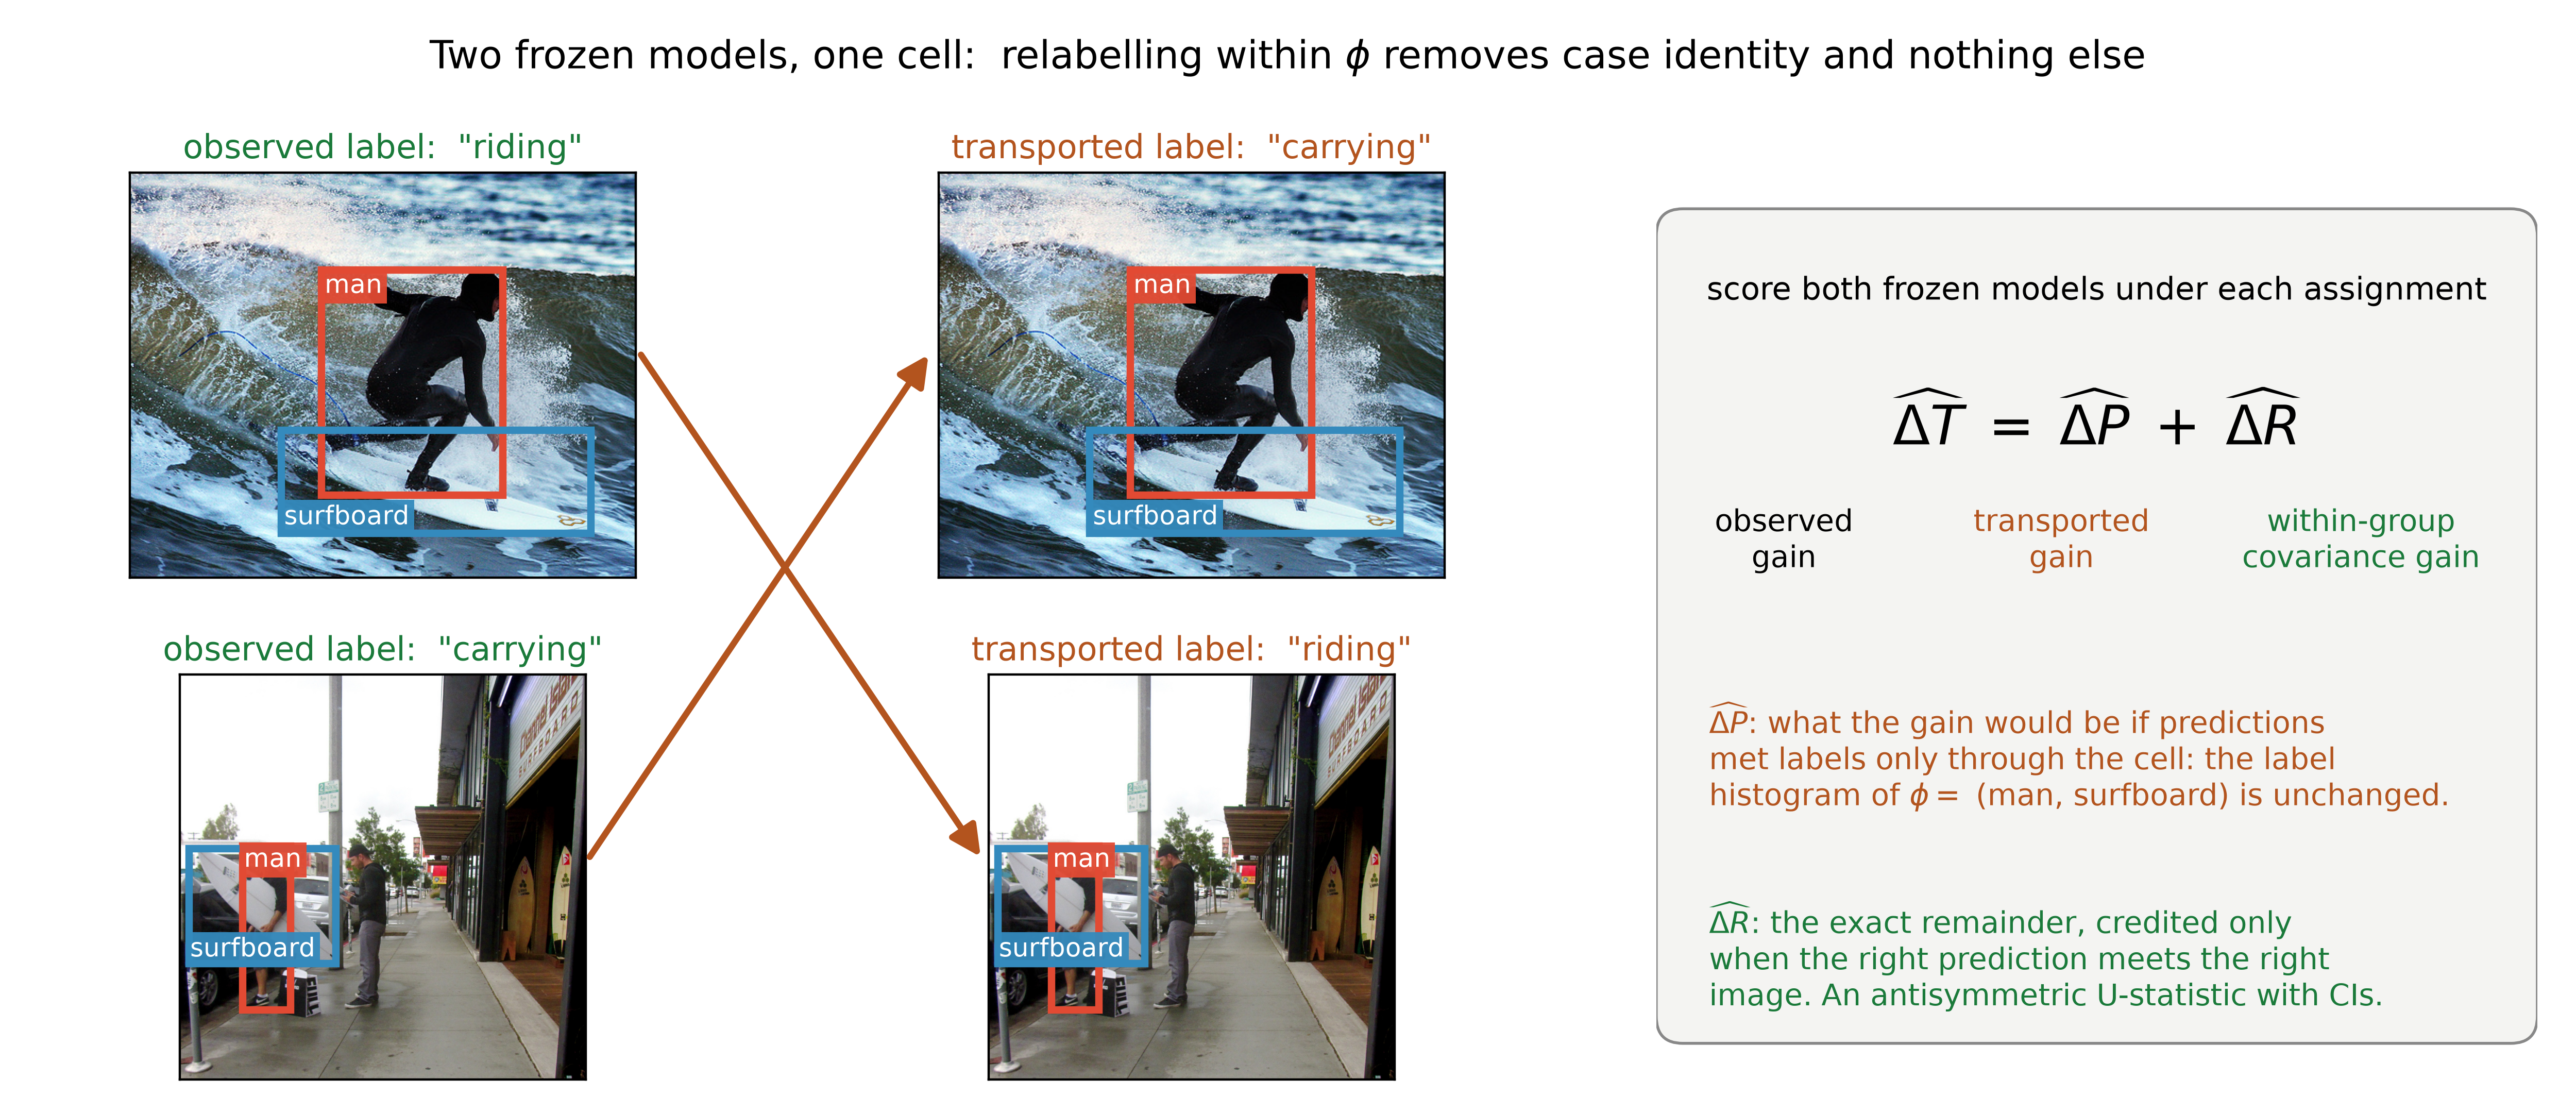
\includegraphics[width=\textwidth]{figures/fig1_new_concept.png}
\caption{\textbf{The construction, on two real test cases.} Two VG150 test relations
share the group $\phi=(\textsf{man},\textsf{surfboard})$ but carry different labels.
Exchanging their labels (arrows) leaves the group and its label frequencies intact while
breaking the link between each prediction and the case it was made for. Scoring two
frozen models before and after the exchange splits their score difference exactly into a
prior-fit gain and a within-group resolution gain.}
\label{fig:concept}
\end{figure*}

\paragraph{What the second component is, in standard terms.}
The surviving component is not a new invention. Written out, the within-group remainder
equals the covariance, inside each group, between how much the new model moved its
predicted probability for a label and whether that label actually occurred
(Theorem~\ref{thm:population}). That covariance is the \emph{resolution} term of the
classical reliability--resolution decomposition of a proper score
\citep{murphy1973vector,degroot1983comparison,brocker2009reliability}, which splits a
single forecaster's score, conditional on a chosen grouping, into how well calibrated it
is and how much its forecasts vary with the outcome. Our contribution is to obtain that
term for a \emph{pair} of forecasters directly, as an exact finite-sample identity with
inference attached, rather than by decomposing each forecaster separately and
subtracting. We call the resulting estimator WAGER (within-group antisymmetric gain
evaluation of resolution) for reference, and name its two components the
\emph{prior-fit gain} and the \emph{within-group resolution gain} throughout.

\subsection{Contributions}\label{sec:contributions}

\begin{enumerate}
\item \textbf{An exact decomposition, and what its remainder is.} For any score, the
observed gain between two frozen models splits exactly --- in the population
(Theorem~\ref{thm:population}) and in the finite sample (Theorem~\ref{thm:sample}) ---
into a prior-fit gain and a remainder that is a U-statistic of order two. For every
Bregman score, and hence for the quadratic and logarithmic scores as named cases, that
remainder equals a within-group covariance between the models' predicted-probability
difference and the label indicator (Theorem~\ref{thm:bregman}). A change that is
constant within groups contributes exactly zero to it.

\item \textbf{Inference for the difference, and its large-sample justification.} We
derive the estimator's influence function, which gives cluster-robust confidence
intervals in one pass over the data, together with a randomization test stratified by
group. The dataset-level estimator is asymptotically normal with a consistent sandwich
variance (Theorem~\ref{thm:clt}); at a trivial grouping variable it reduces exactly to a
clustered Diebold--Mariano test of the paired score differential
(Corollary~\ref{cor:dm}), so the decomposition delivers what that classical test does
plus the split it does not.

\item \textbf{Two exact statements about design choices that would otherwise be
guesswork.} Using a group's own observed label frequency as the counterfactual, rather
than leaving each case out, attenuates the estimate by exactly $(n_c-1)/n_c$ in a group
of size $n_c$ (Proposition~\ref{prop:attenuate}) --- which is why no held-out fold is
needed. Merging groups shifts the estimand by an explicit between-group covariance of
either sign (Proposition~\ref{prop:coarsen}), so a coarser grouping variable cannot be
assumed harmless. A Cauchy--Schwarz bound
(Proposition~\ref{prop:sensitivity}) limits how far an unrecorded grouping variable could
move the reported remainder, from a single elicited correlation.

\item \textbf{Validation, and an audit of a published method.} Simulations establish
interval coverage under clustering and delimit what the two components separate:
prior-only improvements stay out of the resolution component, unrecorded within-group
signal enters it, and monotone recalibration moves score between the components, which is
why we audit calibration-matched pairs. Applied to two publicly released scene-graph
checkpoints --- not to models of our own --- the decomposition shows that a ten-point
improvement in mean recall is overwhelmingly prior-fit under either of two proper scores
(Section~\ref{sec:sggaudit}). Three further studies, in relation prediction and in
long-tailed image and text classification, apply the identical estimator and are reported
in Appendix~\ref{app:studies}.
\end{enumerate}

\subsection{Terminology}\label{sec:terminology}

The construction needs few new words, and Table~\ref{tab:terms} fixes them against their
standard statistical counterparts. Readers who prefer the standard vocabulary can read
``group'' for cell, ``resolution'' for the second component, and ``relabelling within
groups'' for transport, and lose nothing.

\begin{table}[t]
\centering
\small
\caption{The paper's vocabulary, and what it corresponds to in standard terms.}
\label{tab:terms}
\begin{tabular}{@{}p{0.24\textwidth}p{0.30\textwidth}p{0.38\textwidth}@{}}
\toprule
Term used here & Standard counterpart & Meaning \\
\midrule
grouping variable $\phi$ &
stratifying / conditioning variable &
a discrete function of the input, declared before the audit, whose levels the labels
depend on \\
cell $c$ &
level of $\phi$; stratum &
the set of test cases sharing one value of $\phi$ \\
label transport &
within-stratum relabelling; permutation within blocks &
replacing a case's label with another case's label from the same cell \\
total gain $\Delta T$ &
paired score differential &
the observed mean score of the new model minus that of the old \\
prior-fit gain $\Delta P$ &
--- &
the part of $\Delta T$ that survives label transport \\
within-group resolution gain $\Delta R$ &
resolution difference \citep{murphy1973vector,brocker2009reliability} &
the part destroyed by transport; a within-cell prediction--label covariance \\
coverage &
identified fraction &
share of test cases in cells of size $\ge2$, the only cells in which $\Delta R$ is
identified \\
calibration-matched &
temperature-scaled on held-out data &
both models rescaled to comparable confidence before the audit \\
\bottomrule
\end{tabular}
\end{table}

\subsection{Scope, and what is not claimed}\label{sec:scope}

The estimator needs exactly four aligned arrays: two $N\times K$ matrices of predicted
probabilities, the $N$ observed labels, and the $N$ cell identifiers. Any closed-set
probabilistic prediction task supplies them. Free-form or generative evaluation, where no
$K$-way probability vector exists, does not, and we make no claim there.

Three limits on interpretation are worth stating before any result. First, everything is
conditional on the declared $\phi$: a positive $\Delta R$ says the new model predicts
individual cases better \emph{among cases sharing that feature}, and nothing about
causality, reasoning, or robustness. Second, $\Delta R$ credits any signal that varies
within a cell, including a shortcut the analyst did not record;
Proposition~\ref{prop:sensitivity} bounds that exposure rather than removing it. Third, a
prior-fit gain is not illegitimate --- fitting the deployment label distribution better
is real skill whenever that distribution is the one that matters. The decomposition says
where a gain lives, not whether it is worth having.

\paragraph{Organization.}
Section~\ref{sec:worked} works a four-point example. Section~\ref{sec:related} places the
construction in the literature on proper-score decomposition and forecast comparison.
Section~\ref{sec:method} develops the estimator and its theory.
Section~\ref{sec:exp} validates it and audits two released checkpoints.
Sections~\ref{sec:discussion} and~\ref{sec:conclusion} discuss limits and conclude.
Proofs are in Appendix~\ref{app:proofs}; three further empirical studies are in
Appendix~\ref{app:studies}.

\section{Related work}\label{sec:related}

The construction sits between two literatures that rarely meet: the decomposition of
proper scores, which supplies the object being estimated, and the comparison of
forecasters, which supplies the inferential target. We take those first, then the applied
literature that motivates the problem.

\subsection{Relation to classical proper-score decompositions}\label{sec:related-decomposition}

Conditional on a chosen grouping variable, a proper score splits into a calibration
(reliability) term and a resolution term \citep{murphy1973vector,degroot1983comparison}, made
conditioning-set explicit by \citet{brocker2009reliability}, whose treatment already covers
general strictly proper scores and multicategory outcomes.

Our $\Delta R$ is related to that resolution term but is not equal to it, and the distinction
matters before anything is built on it. The representation of a resolution-like quantity as a
\emph{covariance} between forecast and outcome indicator is due to \citet{yates1982external},
whose covariance decomposition of the Brier score is the direct ancestor of
Eq.~\eqref{eq:cov-id}. The classical resolution term of \citet{degroot1983comparison} is a
different object: it depends on a forecast only through the partition generated by its level
sets, so it is invariant under any strictly monotone relabelling of forecast values. A
covariance between forecast values and outcomes has no such invariance. The two coincide ---
$\Delta R_c$ equals twice a difference of classical resolution terms --- exactly when both
models are calibrated within each cell of $\phi$, and otherwise differ by a
reliability--resolution cross term that a monotone recalibration moves.
Section~\ref{sec:simulation} measures the gap: a pure recalibration of one model, which
cannot change either model's classical resolution at all, moves $\widehat{\Delta R}$ by
$-0.488$ and reverses the sign verdict of the audit in Section~\ref{sec:sggaudit}. We
therefore name $\Delta R$ for the covariance it is, and adopt confidence matching as
procedure rather than caveat.

What the classical decomposition does not supply is inference for a pairwise contrast. The
point estimates do combine: both models share the $\phi$-partition and hence the same
per-cell $n_c$, so the same $(n_c-1)/n_c$ attenuation applies to each model's separately
estimated in-sample resolution, and subtracting two naive plug-ins recovers exactly the
biased estimate of the contrast. Inference does not transfer. Variance estimators for the
single-model decomposition \citep{siegert2014variance} target one resolution term in
isolation and supply no covariance between it and a second model's estimate from the same
data. Rebuilding that from the joint law is routine rather than open, and the field is not
silent about it \citep{ferro2007comparing,delsole2014comparing,delong1988comparing}. What is
new is not that a contrast can be given a variance, but that it admits an \emph{exact
finite-sample decomposition} whose remainder is an antisymmetric U-statistic with a one-pass
influence function, so the split and its uncertainty come from one construction.

\subsection{Comparing two forecasters}\label{sec:related-dm}

Inference on a paired score differential is the classical territory of comparative
forecast evaluation: the Diebold--Mariano test \citep{diebold1995comparing} and
conditional predictive ability tests \citep{giacomini2006tests} ask whether one forecaster
beats another, optionally conditional on covariates. That is the closest existing relative
of a gain evaluated conditional on $\phi$, and
Corollary~\ref{cor:dm} makes the relation exact: at the trivial one-cell partition our
total-gain statistic and its interval \emph{are} a clustered Diebold--Mariano test,
corrected for cluster rather than serial dependence. The decomposition is therefore best
read as everything those tests already deliver plus a split that neither provides. A
structurally close precedent for comparing two correlated models through a paired
U-statistic exists outside forecast evaluation as well: \citet{delong1988comparing}
compare two correlated ROC curves' areas via a generalized U-statistic covariance
estimator, the same construction applied to an unconditional ranking statistic rather than
a declared-cell gain.

Two further literatures locate the same object from other directions. The transported
component is precisely what label-shift procedures manipulate post hoc: re-weighting a
classifier's outputs towards a new label distribution
\citep{saerens2002adjusting,lipton2018detecting} can add or remove transported gain without
touching case-level evidence, which Appendix~\ref{app:vgvisual} exploits as a
falsification test. And evaluating calibration within cells of a declared grouping,
uniformly over many candidate groupings, is the subject of multicalibration
\citep{hebert2018multicalibration}, which is the formal treatment of the multiplicity
question raised by the choice of $\phi$ (Section~\ref{sec:discussion}).

\subsection{Transport, permutation, and U-statistics}\label{sec:related-perm}

Strictly proper scoring rules reward honest predictive distributions
\citep{gneiting2007proper}, and permutation methods have long been used to assess classifier
performance \citep{ojala2010permutation}. Conditional permutation tests generally estimate
or assume a conditional distribution when the conditioning variables are continuous or
high-dimensional. The setting here is different in a way that buys exactness: a benchmark
supplies a \emph{discrete} grouping variable, and the target is not generic conditional
independence but one specific model-to-model score gain, so within-cell transport needs no
nuisance law at all. The remainder is a U-statistic of order two in the sense of
\citet{hoeffding1948class}, and its H\'ajek projection is what supplies the influence
function of Section~\ref{sec:inference}. The new element is the gain-contrast transport
identity and the attribution it licenses, not permutation or U-statistic theory by itself.

Two further connections are worth naming. The transported component is what label-shift
procedures manipulate post hoc: re-weighting a classifier's outputs towards a new label
distribution \citep{saerens2002adjusting,lipton2018detecting} can add or remove transported
gain without touching case-level evidence, which Section~\ref{sec:vgvisual} exploits as a
falsification test, and which is why Section~\ref{sec:decision}'s model-selection reversal
is a label-shift argument. And what an unrecorded grouping variable can hide is the subject
of omitted-variable sensitivity analysis \citep{rosenbaum2002observational};
Proposition~\ref{prop:sensitivity} adapts that style of argument to bound how far an
unrecorded covariate could move $\Delta R$.

Usable-information analyses measure information accessible to a chosen predictor family
\citep{xu2020theory}. Their central objects are model- or family-level quantities; ours is
narrower and more operational, attributing the score difference between two concrete frozen
models. A positive $\Delta R$ establishes nothing about causal or compositional structure.

\subsection{Prior-aware evaluation in vision}\label{sec:related-applied}

Dataset bias has long complicated comparisons between recognition systems
\citep{torralba2011unbiased,geirhos2020shortcut}. In scene graph generation a frequency
predictor of $p(\text{predicate}\mid\text{subject},\text{object})$ is surprisingly
competitive \citep{zellers2018neural}; mean recall and causal interventions were proposed to
reduce that dependence \citep{chen2019knowledge,tang2019learning,tang2020unbiased}, though
metric pathologies remain \citep{li2022rethinking} and the same diagnosis recurs in
open-vocabulary and knowledge-enhanced work
\citep{li2024pixels,zhang2024hiker,sun2024unbiased}. In visual question answering, GQA-OOD
stratifies by answer rarity within question groups \citep{kervadec2021roses} and VQA-CP
changes language priors between train and test \citep{agrawal2018dont}, though
changing-prior splits can themselves be exploited \citep{teney2020value}; the shortcut is
still targeted directly \citep{xu2025qirl,kuang2024debiasing}, and benchmark-level audits of
exploitable non-visual shortcuts have widened to multimodal evaluation generally
\citep{brown2025benchmark,zhou2025shortcut}. In long-tailed recognition a classifier can
raise aggregate accuracy by fitting training class frequencies more precisely without
discriminating better within a class \citep{ma2024geometric,duan2024longtailed}; the
canonical remedies rebalance the objective or the classifier
\citep{cui2019classbalanced,cao2019learning,menon2021long,kang2020decoupling}, with a
continuing stream of variants \citep{li2026pih2t,luo2025rebalancing}.

Reporting standards have responded to the shortcut: mean recall alongside recall, often
broken down by predicate frequency \citep{tang2020unbiased,li2022rethinking}, and zero-shot
recall \citep{lu2016visual} checking whether a gain survives on triplets absent from
training. These are effective prior-aware slicings, splits and stress tests of a
\emph{single} model's performance. What none provides is what we target: an exact
decomposition, with uncertainty, of the score difference between two fixed systems. A
stratified or zero-shot metric can show \emph{that} a gain is uneven across the prior; it
does not attribute the pairwise gain itself, on the full evaluation set, with a
finite-sample identity and inference. The remedies, equally, intervene on how a model is
trained rather than on how a trained pair is compared.

\section{The estimator and its properties}\label{sec:method}

This section states the construction of Sections~\ref{sec:intro}--\ref{sec:worked}
formally and establishes its properties. The order is: notation and the object being
decomposed (Section~\ref{sec:setup}); the population identity and the covariance form of
its remainder (Section~\ref{sec:transport}), which Section~\ref{sec:bregman} shows is not
specific to the quadratic score; what happens when the grouping variable is made coarser
(Section~\ref{sec:coarsening}) or is missing a relevant covariate altogether
(Section~\ref{sec:sensitivity}); the finite-sample identity and its $O(NK)$ computation
(Sections~\ref{sec:finite}--\ref{sec:efficient}); why the counterfactual leaves each case
out rather than fitting the group's own frequencies (Section~\ref{sec:attenuation}); and
inference, both finite-sample and asymptotic
(Sections~\ref{sec:inference}--\ref{sec:asymptotic}). Proofs are in
Appendix~\ref{app:proofs}. A reader who wants only what is needed to use the estimator can
read Sections~\ref{sec:setup}, \ref{sec:transport}, \ref{sec:finite}
and~\ref{sec:inference} and skip the rest.

\subsection{Setup: what is being decomposed}\label{sec:setup}

Let $q_0(\cdot\mid x)$ and $q_1(\cdot\mid x)$ be the predictive distributions of an
old and a new frozen model over $K$ labels. Let $S(q,y)$ be a bounded proper score,
oriented so that larger is better, and let $C=\phi(X)$ be a declared discrete
grouping variable. In the relation-prediction example of Section~\ref{sec:intro}, $C$ is the ordered
subject--object class pair; in a long-tailed classification benchmark it is a coarse
superclass. We call a value of $C$ a \emph{cell} and require it to be declared before the
audit is run. Define the
instance-specific \emph{gain vector}
\begin{equation}
H_x(y)=S(q_1(\cdot\mid x),y)-S(q_0(\cdot\mid x),y),\qquad y=1,\ldots,K.
\label{eq:gain-vector}
\end{equation}
Unlike the realized gain $H_X(Y)$, this vector can be evaluated at a counterfactual
label without rerunning either model.

Our default is the quadratic score
\begin{equation}
S_{\rm B}(q,y)=2q_y-\lVert q\rVert_2^2,
\label{eq:brier}
\end{equation}
which differs from negative Brier loss only by a label-only constant. It is strictly
proper and bounded, avoids probability clipping, and uses the entire predictive
distribution. A floored log score is a sensitivity analysis.

\subsection{Within-cell counterfactual transport}\label{sec:transport}

For a cell $c$, define three population quantities:
\begin{align}
\Delta T_c &= \mathbb E[H_X(Y)\mid C=c], \\
\Delta P_c &= \mathbb E_{H\mid c}\,\mathbb E_{Y'\mid c}[H_X(Y')], \\
\Delta R_c &= \Delta T_c-\Delta P_c .
\end{align}
Here $Y'$ is an independent label drawn from the same cell. Thus $\Delta T_c$ is the
observed score gain, $\Delta P_c$ is the gain retained after breaking the
instance-specific prediction--label assignment while preserving the cell, and
$\Delta R_c$ is the covariance gain lost by that transport.

\begin{theorem}[Transport and covariance identities]\label{thm:population}
For any integrable score contrast $H$,
\begin{equation}
\Delta T_c=\Delta P_c+\Delta R_c,
\qquad
\Delta R_c=\sum_{y=1}^K
\operatorname{Cov}\!\left(H_X(y),\ind \{Y=y\}\mid C=c\right).
\label{eq:population-id}
\end{equation}
For the quadratic score, writing $\Delta q_y(X)=q_1(y\mid X)-q_0(y\mid X)$,
\begin{equation}
\Delta R_c=2\sum_{y=1}^K
\operatorname{Cov}\!\left(\Delta q_y(X),\ind \{Y=y\}\mid C=c\right).
\label{eq:cov-id}
\end{equation}
Consequently, if the gain vector is a function of $c$ alone, then $\Delta R_c=0$.
\end{theorem}

Equation~\eqref{eq:cov-id} is the operational meaning of the construction: the new model
receives covariance credit only to the extent that its probability change aligns more
strongly with the label of the correct case within the same cell. Cell-constant score
improvements, including a better fit to the cell's label histogram, remain in $\Delta P$. A
nonzero covariance does not assert causal or compositional understanding; unrecorded
within-cell shortcuts contribute to it too, so $\phi$ must be declared and stress-tested.

\subsection{What the transported gain measures}\label{sec:transported}

The surviving component is easy to misname. It is tempting to call $\Delta P$ a prior-fit
gain, since transport replaces a case's label by an independent draw from its cell; earlier
drafts of this paper did. Proposition~\ref{prop:transported} in
Appendix~\ref{app:transported} shows the name is wrong and says what the quantity is
instead: under the quadratic score $\Delta P_c$ equals the improvement in how closely the new
model's \emph{mean} within-cell forecast sits to the cell's label frequencies, minus the
increase in the within-cell dispersion of its forecasts. Only the first term is prior fit.
The second rewards the new model for making less dispersed predictions at a fixed mean
forecast, so $\Delta P$ can absorb an entire observed gain with both models' mean forecasts
sitting exactly on the cell frequencies --- a four-point counterexample in that appendix does
just that. This is the reliability-and-sharpness channel of the classical partition, not a
prior-fitting channel, which is why we name it for the operation that produces it; it is also
why confidence matching moves $\widehat{\Delta P}$ so sharply, since a temperature change is
almost purely a change in dispersion.

\subsection{Generalization: the Bregman-score family}\label{sec:bregman}

Nothing in the proof of Theorem~\ref{thm:population} uses properness: the identity and the
covariance sum follow from the definitions alone, for any score. What is specific to the
quadratic score is the further reduction to Eq.~\eqref{eq:cov-id}, in which the part of
$H_x(y)$ not depending on $y$ integrates out because $\sum_y\ind\{Y=y\}=1$ almost surely.
The same cancellation occurs for every strictly proper score generated by a Bregman
divergence, so Eq.~\eqref{eq:cov-id} and the log-score identity used as a robustness check
in Section~\ref{sec:sggaudit} are two instances of one theorem. For a strictly convex,
differentiable $\psi$ on the simplex, the Bregman score is
$S_\psi(q,y)=\psi(q)+\langle\nabla\psi(q),e_y-q\rangle$; taking $\psi(q)=\lVert q\rVert_2^2$
recovers the quadratic score and $\psi(q)=\sum_kq_k\log q_k$ the log score
\citep{gneiting2007proper}.

\begin{theorem}[Bregman-score covariance identity]\label{thm:bregman}
Let $H_x(y)=S_\psi(q_1(\cdot\mid x),y)-S_\psi(q_0(\cdot\mid x),y)$ for a Bregman score generated by a strictly convex, differentiable $\psi$, and write $\Delta g_y(x)=\partial_y\psi(q_1(\cdot\mid x))-\partial_y\psi(q_0(\cdot\mid x))$ for the contrast of the $y$-th gradient coordinate. Then
\begin{equation}
\Delta R_c=\sum_{y=1}^K\operatorname{Cov}\!\bigl(\Delta g_y(X),\,\ind\{Y=y\}\mid C=c\bigr).
\label{eq:bregman-cov-id}
\end{equation}
\end{theorem}

\begin{corollary}[Quadratic and log score]\label{cor:bregman}
For $\psi(q)=\lVert q\rVert_2^2$, $\Delta g_y(x)=2\Delta q_y(x)$ and Eq.~\eqref{eq:bregman-cov-id} is Eq.~\eqref{eq:cov-id}. For $\psi(q)=\sum_kq_k\log q_k$, $\Delta g_y(x)=\log q_1(y\mid x)-\log q_0(y\mid x)$, and
\begin{equation}
\Delta R_c=\sum_{y=1}^K\operatorname{Cov}\!\left(\log\frac{q_1(y\mid X)}{q_0(y\mid X)},\ \ind\{Y=y\}\ \middle|\ C=c\right).
\label{eq:log-cov-id}
\end{equation}
\end{corollary}

Eq.~\eqref{eq:log-cov-id} gives the log-score check of Section~\ref{sec:sggaudit} the same exact covariance meaning that Eq.~\eqref{eq:cov-id} gives the quadratic score: within-group covariance under the log score is the within-cell covariance between the log-likelihood-ratio contrast of the two models and the observed label indicator, not merely "a sensitivity analysis." Any other Bregman score -- the spherical or power-family scores catalogued by \citet{gneiting2007proper}, for instance -- inherits an identity of the same form through its own $\psi$, so Theorem~\ref{thm:bregman} fixes the scope of the estimator's scoring-rule dependence once, rather than leaving each alternative score to be checked separately. The implemented log score floors each probability at $\epsilon=10^{-6}$ to avoid $-\infty$ on an unseen label; Eq.~\eqref{eq:log-cov-id} is exact for the unfloored $\log q_y$, and the floored version used throughout is a sensitivity check on that exact identity rather than a literal instance of it, negligibly different whenever no relevant probability is within $\epsilon$ of zero.

\subsection{Coarsening the cell}\label{sec:coarsening}

Appendix~\ref{sec:ablations} reports that replacing the class-pair cell with a coarser
subject-only cell changes the estimated covariance gain. The following result gives that
sensitivity an exact population-level mechanism rather than treating it as an empirical
curiosity.

\begin{proposition}[Coarsening decomposition]\label{prop:coarsen}
Let $\bar\phi=g(\phi)$ be any coarsening of the grouping variable, so that each cell
$\bar c$ of $\bar\phi$ is a union of cells of $\phi$. Then
\begin{equation}
\Delta R_{\bar c}
=\mathbb E\!\left[\Delta R_C \mid \bar\phi=\bar c\right]
+\sum_{y=1}^K\operatorname{Cov}\!\left(\mathbb E[H_X(y)\mid C],\,
\Pr(Y=y\mid C)\ \middle|\ \bar\phi=\bar c\right).
\label{eq:coarsen}
\end{equation}
\end{proposition}

The first term is the coarse cell's share of the fine-grained covariance gain; the second is
a between-cell covariance, over the finer cells nested inside $\bar c$, between each fine
cell's typical gain at label $y$ and its label-$y$ frequency. It is not sign definite, so
coarsening $\phi$ can inflate or deflate the credited covariance gain, and it vanishes
exactly when either quantity is constant within each coarse cell. This is why the finest
defensible $\phi$ is the conservative default: coarsening adds cross-cell prior structure
into $\Delta R$, while the finer partition's gain is preserved on average through the first
term. The proof is a per-label application of the law of total covariance
(Appendix~\ref{app:proofs}).

\subsection{Sensitivity to an unrecorded confounder}\label{sec:sensitivity}

Read in one direction, Proposition~\ref{prop:coarsen} says what folding a covariate into
$\phi$ does. Read in the other, it quantifies what happens when a relevant covariate is
\emph{never} declared, which is the estimator's main scope limit. Let $Z$ be unrecorded and
let $(\phi,Z)$ be the finer, fully adjusted cell. Applying
Proposition~\ref{prop:coarsen} with $\bar\phi=\phi$ gives, for every declared cell $c$,
\begin{equation}
\Delta R_c(\phi)=\mathbb E\!\left[\Delta R_{(\phi,Z)}\mid\phi=c\right]
+\sum_{y=1}^K\operatorname{Cov}\!\left(\mathbb E[H_X(y)\mid\phi,Z],\,
\Pr(Y=y\mid\phi,Z)\ \middle|\ \phi=c\right),
\label{eq:sensitivity-exact}
\end{equation}
whose first term is what an analyst who could observe $Z$ would report and whose second is
the bias of using $\phi$ alone. The identity is exact but needs $Z$'s joint law with
$(H,Y)$. The following bound replaces that with a judgement about how strongly an unrecorded
variable could plausibly act, in the spirit of \citet{rosenbaum2002observational}.

Proposition~\ref{prop:sensitivity} in Appendix~\ref{app:sensitivity} states the bound: for a
single elicited correlation $\bar\rho$ between an unrecorded variable's effect on the
within-cell gain and its effect on the within-cell label distribution, the bias of using
$\phi$ alone is at most $\bar\rho$ times a product of two dispersion factors, with a
data-free form $\bar\rho M\sqrt{K-1}$ needing only the label cardinality and the score
bound. Because $\bar\rho$ is a correlation rather than a domain-specific odds ratio, it can
be elicited the same way across benchmarks. Appendix~\ref{app:sensitivity} evaluates both
forms on our own estimates, and the sharp one is the less comfortable: an unrecorded
covariate correlated at $0.061$ would account for the entire covariance gain reported in
Section~\ref{sec:results}.

\subsection{Exact finite-sample decomposition}\label{sec:finite}

Consider cell $c$ with $n_c\ge2$ examples. Write $H_i(y)=H_{x_i}(y)$. WAGER computes
\begin{align}
\widehat{\Delta T}_c
 &=\frac1{n_c}\sum_{i\in c} H_i(y_i), \\
\widehat{\Delta P}_c
 &=\frac1{n_c(n_c-1)}\sum_{i\ne j\in c}H_i(y_j),
\label{eq:sample-prior}\\
\widehat{\Delta R}_c
 &=\binom{n_c}{2}^{-1}\sum_{i<j\in c} A_{ij},
\label{eq:sample-reason}
\end{align}
where the antisymmetric kernel is
\begin{equation}
A_{ij}=\frac12\{H_i(y_i)+H_j(y_j)-H_i(y_j)-H_j(y_i)\}.
\label{eq:kernel}
\end{equation}

\begin{theorem}[Finite-sample WAGER identity]\label{thm:sample}
For every cell with $n_c\ge2$, without a distributional assumption,
\begin{equation}
\widehat{\Delta T}_c=\widehat{\Delta P}_c+\widehat{\Delta R}_c.
\end{equation}
Moreover, when the cell's examples are drawn i.i.d.\ from the cell population,
$\widehat{\Delta R}_c$ is an unbiased order-two U-statistic for $\Delta R_c$.
Independence, not exchangeability alone, is what unbiasedness requires: the
independent-coupling definition of $\Delta P_c$ pairs an example with a label drawn
independently from the same cell, so $\mathbb E[H_1(Y_2)]$ matches it only for
independent within-cell draws.
\end{theorem}

Dataset-level quantities weight cells by their identified counts,
$\widehat{\Delta Z}=N_*^{-1}\sum_{c:n_c\ge2}n_c\widehat{\Delta Z}_c$ for $Z\in\{T,P,R\}$.
Singleton cells cannot identify a within-cell counterfactual, so we exclude and report them
rather than inventing a smoothed estimate. If $\widehat{\Delta T}>0$ the descriptive share
$\widehat{\Delta R}/\widehat{\Delta T}$ may exceed one, when covariance improves while the
transported channel deteriorates, and it is undefined for a nonpositive total; we therefore
report $\widehat{\Delta R}$ as the primary result rather than a thresholded ratio.

\subsection{Linear-time computation}\label{sec:efficient}

Naively evaluating Eq.~\eqref{eq:sample-prior} is quadratic in cell size. Let $m_{cy}$
be the count of label $y$ in cell $c$. For example $i\in c$, its transported score is
\begin{equation}
P_i=\frac{\sum_{y=1}^K m_{cy}H_i(y)-H_i(y_i)}{n_c-1}.
\label{eq:linear}
\end{equation}
Averaging $P_i$ yields Eq.~\eqref{eq:sample-prior}; averaging
$H_i(y_i)-P_i$ yields Eq.~\eqref{eq:sample-reason}. Thus the entire estimator costs
$O(NK)$ time and $O(NK)$ storage for cached prediction vectors. No model fitting,
projection fold, hierarchy, or smoothing hyperparameter appears.

\subsection{Why leave-one-out transport, not a fitted-in-sample prior}\label{sec:attenuation}

Equation~\eqref{eq:linear} excludes example $i$'s own label from its transported score.
It is natural to ask what is lost by the simpler alternative of fitting the cell's
empirical label frequency on all $n_c$ examples, including $i$, and using that fitted
frequency as the counterfactual, i.e.\ treating $\hat p_c(y)=m_{cy}/n_c$ as a prior model
and setting $\tilde P_i=\sum_y \hat p_c(y)H_i(y)=n_c^{-1}\sum_y m_{cy}H_i(y)$. This is
the natural plug-in estimator, and it is what a frequency-collapsed projection baseline
computes when no separate evaluation fold is withheld from fitting.

\begin{proposition}[Exact attenuation of the in-sample plug-in]\label{prop:attenuate}
For every cell with $n_c\ge2$ and every $i\in c$, writing $\hat P_i$ for
Eq.~\eqref{eq:linear} and $\hat R_i=H_i(y_i)-\hat P_i$,
\begin{equation}
\tilde P_i=\hat P_i+\frac1{n_c}\hat R_i,
\qquad
\tilde R_i:=H_i(y_i)-\tilde P_i=\frac{n_c-1}{n_c}\,\hat R_i.
\label{eq:attenuation}
\end{equation}
Consequently the in-sample plug-in's dataset-level statistic obeys
$\widetilde{\Delta R}=N_*^{-1}\sum_{c:n_c\ge2}(n_c-1)\widehat{\Delta R}_c$, a
multiplicative shrinkage of every cell's leave-one-out covariance gain by the factor
$(n_c-1)/n_c$.
\end{proposition}

The shrinkage is deterministic, not a variance statement: whenever
$\widehat{\Delta R}_c\neq0$ the in-sample plug-in is biased for it at every finite $n_c$,
worst in the smallest identified cells ($50\%$ at $n_c=2$). The standard remedy for such
self-prediction bias is a projection/evaluation split, which restores unbiasedness by
discarding examples from both stages and introduces a split-fraction hyperparameter and
typically higher variance. Leave-one-out transport removes the bias exactly, at the full
sample, for every cell with $n_c\ge2$, with no fitted nuisance distribution at all.

\subsection{Inference}\label{sec:inference}

For point estimation we use all unordered within-cell pairs. For uncertainty, define
$\bar A_i=(n_c-1)^{-1}\sum_{j\ne i}A_{ij}$ and
$\widehat{\Delta R}_c=n_c^{-1}\sum_i\bar A_i$. The estimated H\'ajek influence
contribution for random cell membership is
\begin{equation}
\widehat\psi_i=2\bar A_i-\widehat{\Delta R}_c-\widehat{\Delta R}.
\label{eq:influence}
\end{equation}
We sum $\widehat\psi_i$ within image and use the resulting one-way sandwich variance,
so multiple relations from the same image are not treated as independent. Total-gain
influence is $H_i(y_i)-\widehat{\Delta T}$; prior-gain and share intervals follow from
the exact identity and delta method.

As a complementary finite-group diagnostic, WAGER applies an independently sampled
cyclic shift to labels inside every cell. Each shift preserves cell size and label
histogram. Recomputing $\widehat{\Delta R}$ under $B$ shifts gives
\begin{equation}
p=\frac{1+\sum_{b=1}^B\ind \{\widehat{\Delta R}^{(b)}\ge
\widehat{\Delta R}\}}{B+1}.
\end{equation}
This is exact under the sharp null that labels are exchangeable relative to the frozen
model outputs within each cell. Because SGG relations share images, our primary
real-data uncertainty statement is the image-cluster-robust interval; the randomization
test is reported as a secondary relation-level diagnostic.

\subsection{Asymptotic normality}\label{sec:asymptotic}

The influence function and sandwich variance behind the reported intervals are derived in
Appendix~\ref{app:influence} through a H\'ajek-projection expansion. The following supplies
the limit theorem, under conditions that hold whenever the score is bounded and no cluster
dominates the sample.

Theorem~\ref{thm:clt} in Appendix~\ref{app:clt} states it: if the score is bounded, examples
fall in mutually independent clusters none of which dominates the sample, the number of
eligible cells is negligible against the identified sample, and $\phi$ has fixed finite
support whose every cell grows, then $\sqrt{N_*}(\widehat{\Delta R}-\theta)$ is
asymptotically normal around the identified-subpopulation estimand and the implemented
sandwich variance is consistent for its limiting variance. The last condition is an
idealisation no heavy-tailed benchmark attains in sample, which is why
Section~\ref{sec:simulation}'s coverage simulation, not this theorem, is what licenses
reading the reported intervals at finite $N$.

\paragraph{Relation to comparative forecast evaluation.}
\begin{corollary}[Relation to Diebold--Mariano/Giacomini--White]\label{cor:dm}
Under the trivial partition $\phi\equiv\text{const}$ (one cell containing every
example), $\widehat{\Delta T}=N^{-1}\sum_iH_i(y_i)$ is the sample mean of the paired loss
differential between the two models, and Theorem~\ref{thm:clt} applied to $\widehat{\Delta T}$
with its image-clustered interval is the grouped, cluster-robust form of the
Diebold--Mariano statistic for that differential \citep{diebold1995comparing}; because
the conditioning information set is empty, it is equivalently a degenerate instance of
the Giacomini--White conditional predictive-ability test \citep{giacomini2006tests}.
\end{corollary}
The corollary is immediate from the definitions: DM and GW test whether a paired loss
differential's mean is zero, and $\widehat{\Delta T}$ at the trivial partition is exactly
that differential's sample mean. Neither test forms $\widehat{\Delta P}$ or
$\widehat{\Delta R}$; both target $\Delta T$ and stop. One qualification on how far the
reading travels: the corollary is stated at the trivial partition, whereas the totals
reported at a nontrivial $\phi$ are $N_*$-weighted means over the \emph{identified}
subsample. Because $\Delta T$ does not depend on $\phi$ except through that exclusion, each
reported $\widehat{\Delta T}$ is a clustered DM statistic for the paired differential on its
identified subsample, which at the coverages here ($99.0\%$ on VG150, $98.9\%$ in
Section~\ref{sec:sggaudit}) differs from the full-sample statistic only in the excluded
singletons.


\section{Validation and an audit of a published method}\label{sec:exp}

Two questions have to be answered before the decomposition can be used on anything, and
they are answered here in that order. Does the estimator recover what it claims to, with
intervals that cover --- and what, precisely, does it fail to separate?
Section~\ref{sec:simulation} answers both under controlled alternatives where the truth is
known by construction. Then, does it say anything a benchmark's own metrics do not?
Section~\ref{sec:sggaudit} puts it to two publicly released checkpoints of a widely cited
debiasing method, chosen so that the audited models are not ours and the claimed
improvement is one the field already reports. Three further studies --- our own Visual
Genome predictors, a frozen-CLIP variant of them, and long-tailed image and text
classification --- apply the identical estimator and are reported in
Appendix~\ref{app:studies}; Section~\ref{sec:further} summarizes what they add. All
confidence intervals are $95\%$.
\subsection{Controlled validation}\label{sec:simulation}

We generate 24 cells over five labels, drawing each cell's label distribution from
a Dirichlet law and taking the old model to be exactly the cell prior. The new model
interpolates toward an oracle, $q_1=(1-\beta)q_0+\beta q_{\rm oracle}$ with
$q_{\rm oracle}$ placing $0.98$ on the realized label, and forty repetitions are run at
each $\beta\in\{0,.1,\ldots,.8\}$. Across that range the estimated covariance gain grows
linearly and monotonically with the injected signal (Figure~\ref{fig:simulation}, left).

Type-I behaviour is assessed by perturbing the prior predictions with mean-zero noise
and then randomly reassigning the perturbed vectors within each cell, which guarantees
that no systematic prediction--label alignment survives. Over 200 such datasets the
99-shift randomization test rejects in $0.030$ of runs at level $0.05$, with a mean
estimated covariance gain of $-8.97\times10^{-5}$; the null $p$-values come out
approximately uniform and the null estimates stay centred at zero
(Figure~\ref{fig:simulation}, centre and right).

\paragraph{Coverage of the primary interval.} The oracle-signal and null designs above
validate the estimator's centering and the randomization diagnostic, but the paper's
primary uncertainty statement is the image-clustered H\'ajek interval, so we validate
its coverage directly in the regime that stresses it: relations grouped into images
(one to about thirty per image) whose oracle weight shares a latent per-image effect,
and Zipf-distributed cell sizes in which most identified cells hold exactly two
examples. Against the design expectation estimated from 4{,}000 independent
replications, the cluster-robust interval covers in $94.0\%$ of 500 runs, while an
interval that wrongly treats relations as independent covers in only $88.6\%$ --
quantifying both the mild finite-sample undercoverage of the asymptotic interval and
the necessity of clustering.

\paragraph{Discriminant validity.} Three further designs test that the channels
separate what they claim to separate. First, a \emph{calibration-only} alternative:
the new model is a temperature-softened copy of an overconfident informative model, so
the pair contains identical instance information. The raw decomposition credits it with
a large negative covariance gain (mean $-0.488$) -- the confound quantified on real
models in Appendix~\ref{app:lt} -- while the calibration-matched protocol below reduces
it to $-0.0003$ (sd $0.0017$ over 200 runs), confirming that the protocol removes
exactly the confidence-scaling channel. Second, a \emph{prior-only} improvement (the
new model corrects a heteroscedastically noisy estimate of the cell prior, adding no
instance information) yields a covariance gain centred at zero ($0.0002$, sd $0.0035$)
with a clearly positive transported channel: prior improvements do not leak into
$\widehat{\Delta R}$ beyond the algebraic guarantee of Theorem~\ref{thm:population}.
Third, an \emph{unrecorded within-cell shortcut} (a binary feature, varying inside each
cell, that shifts the label distribution and is used by the new model) is credited to
covariance ($+0.041$, sd $0.004$), quantifying the stated limitation that
$\widehat{\Delta R}$ measures all within-cell predictive signal relative to the
declared $\phi$, shortcut or otherwise, and cannot by itself distinguish the two.

\paragraph{The calibration-matched protocol.} The third of those designs identifies a
limitation serious enough to be part of the procedure rather than a caveat about it.
Because $\Delta R$ is a covariance between probability movements and labels
(Theorem~\ref{thm:population}), rescaling a fixed model's confidence moves score between
the two components while adding no information about any individual case: a monotone
transformation of the predictions changes the decomposition even though it changes no
ranking and no decision. We therefore adopt the following control wherever the compared
models differ visibly in confidence. Split the evaluation units --- images, where
examples are clustered --- at random into halves. On the first half, fit each model a
single temperature $T$ by maximum held-out likelihood on $q^{1/T}$ renormalized. On the
second half, apply each model's own fitted temperature and run the decomposition there.
The protocol costs nothing but a data split, it uses no label information from the
audited half, and it is what the simulation above shows removes the confidence-scaling
channel almost exactly.

How many splits each study averages over differs, and the difference is worth stating
rather than glossing. The long-tailed classification study of Appendix~\ref{app:lt}
averages over twenty random splits. The audit of Section~\ref{sec:sggaudit} and the
matched rows of Appendix~\ref{app:vgvisual} each use a single split at a fixed seed. For
those two the split is a source of variability the reported interval does not include, and
it is not negligible: the calibration-only arm above has a between-split standard
deviation of $0.001725$, exceeding the half-width of the audit's own reported interval
($0.00115$). The audit's conclusion does not turn on this --- its estimate is
indistinguishable from zero and stays so under any split --- but a reader comparing
interval widths across our tables should know that two of the three matched studies report
within-split uncertainty only. It does not make $\Delta R$ invariant to recalibration in
general; it fixes the confidence scale at which the comparison is made, which is what a
comparison of two \emph{fixed} models needs.

\begin{figure*}[t]
\centering
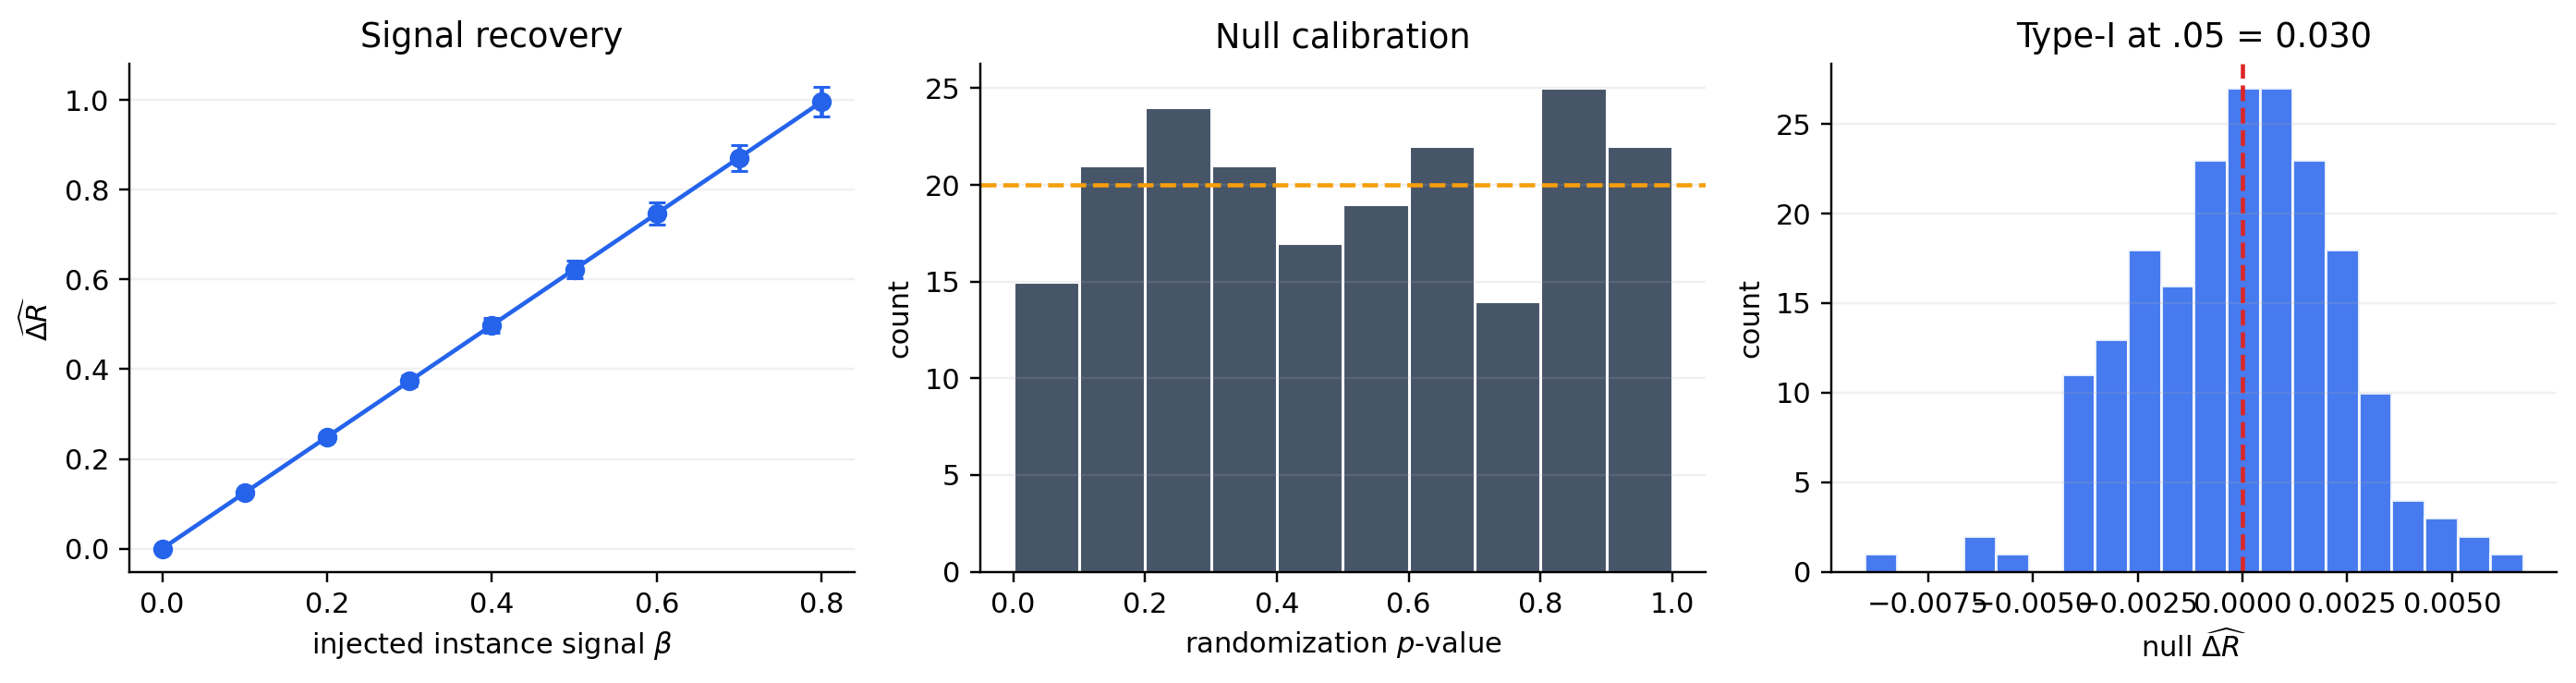
\includegraphics[width=\textwidth]{figures/fig3_new_simulation.png}
\caption{\textbf{Controlled validation.} WAGER recovers injected within-cell signal
monotonically (mean $\pm$ one standard deviation), produces approximately uniform null
randomization $p$-values, and controls type-I error in 200 null runs.}
\label{fig:simulation}
\end{figure*}

\subsection{Auditing a published debiasing method}\label{sec:sggaudit}

The question the decomposition exists to answer concerns systems that other people
release and that the field already compares, so the primary application is to a published
pair rather than to predictors of our own. Tang et al.\ \cite{tang2020unbiased} release a causal MOTIFS PredCls
checkpoint that yields two models from one set of weights: the biased baseline
(MOTIFS-SUM) and its Total Direct Effect counterpart (MOTIFS-TDE), which subtracts a
context-only counterfactual at inference. TDE is among the most cited debiasing methods
in scene graph generation, and it is reported through mean recall, so it is exactly the
kind of claimed improvement whose composition is at issue.

We evaluate both variants with the authors' own code on the canonical VG150 test split,
which fixes the vocabulary, the split and the relation set, and makes the two prediction
sets aligned relation-for-relation by construction. Our reproduction matches the
published behaviour: the baseline reaches $R@50=0.6612$ with $mR@50=0.1459$, and TDE
trades the former for the latter, reaching $R@50=0.4588$ with $mR@50=0.2476$ and raising
zero-shot recall from $zR@50=0.1102$ to $0.1432$. Top-1 predicate accuracy falls from
$0.6981$ to $0.5577$. The audit uses $183{,}639$ relations over $26{,}446$ images and
$7{,}127$ class-pair cells, of which $98.9\%$ are identified.

\paragraph{What is audited, precisely.} One point of bookkeeping before the numbers, since
it changes what the headline row is a statement about. The rows labelled
calibration-matched do not decompose the released checkpoints as released; they decompose
the two models after each has been rescaled by its own temperature ($T^*=2.50$ for the
baseline, $0.92$ for TDE) fitted on a held-out half of the images. That is the comparison
we argue is meaningful, because a proper score punishes miscalibration and these two
models differ sharply in it. But the released pair, scored as it ships, gives a
\emph{significant} covariance loss ($-0.01355$, interval excluding zero), and a
practitioner who downloads those weights and scores them is looking at the raw rows. We
report both and label which is which.

\paragraph{Result.} Table~\ref{tab:sggaudit} decomposes the pair. Read raw, TDE loses
$0.11651$ of quadratic score, of which $0.10296$ sits in the transported channel and a small
but significant $0.01355$ in within-group covariance. That reading does not survive the
control this paper insists on. The two models differ sharply in confidence --- the
baseline is overconfident at $T^*=2.50$ while TDE, having subtracted a counterfactual,
is already near-calibrated at $T^*=0.92$ --- and once temperatures are fitted on a
held-out half of the images and the audit runs on the other half, the quadratic-score
covariance channel is indistinguishable from zero: $\widehat{\Delta R}=-0.00006$ with a
$95\%$ interval of $[-0.00120,+0.00109]$ and a randomization $p$ of $.555$. Essentially
the entire proper-score difference, $-0.18258$ of $-0.18264$, is transported.

The log-score row of the same calibrated comparison does not repeat this null: it
returns $\widehat{\Delta R}=+0.04396$, $95\%$ CI $[+0.04079,+0.04714]$, an interval that
excludes zero. The two proper scores therefore disagree on whether any real covariance
change survives calibration matching -- one reads exactly null, the other reads small
but significantly positive -- while agreeing that whichever value is correct is far
smaller than the calibrated prior-channel shift ($-0.18258$ under the quadratic score,
$-0.59157$ under the log score, both an order of magnitude or more larger than either
covariance estimate). We do not adjudicate between the two scores here: nothing in
Section~\ref{sec:setup} privileges one proper score's covariance estimate as the
``true'' one, and this is the reason the paper's default score is stated as a
declared choice rather than derived. The claim this audit actually supports is the one
both scores agree on --- that TDE's proper-score improvement over the baseline is
overwhelmingly transported \emph{at the calibration-matched, class-pair configuration},
with a covariance remainder at most a small fraction of the total and possibly exactly
zero --- not the stronger, single-score claim that within-group covariance is unchanged.

That qualifier is load-bearing, and we would rather state its force than let a reader
discover it in the table. Table~\ref{tab:sggaudit}'s five configurations of this one pair
give covariance gains of $-0.21711$, $-0.12619$, $-0.01355$, $-0.00006$ and $+0.04396$.
At two of the five, ``overwhelmingly transported'' is simply false: the raw log-score row
has $|\widehat{\Delta R}|=0.126$ against $|\widehat{\Delta P}|=0.159$, and the
subject-only row has $\widehat{\Delta R}=-0.217$ dominating $\widehat{\Delta P}=+0.102$.
We report all five and argue for one on stated grounds --- matched confidence, because a
proper score punishes miscalibration; the finest defensible cell, because
Proposition~\ref{prop:coarsen} makes coarsening non-neutral --- rather than presenting the
favourable configuration as the finding. Theorem~\ref{thm:bregman} is the reason the
score-dependence is not a defect to be argued away: each Bregman generator defines its own
exact estimand, so two proper scores disagreeing about $\Delta R$ are answering two
well-posed questions, and which one an evaluator wants is a declaration, not a fact about
the models.

This is a precise and, we think, fair characterization of what TDE does. Its own
construction subtracts the context-only prediction, so a method that operates on the
transported channel is what its authors built; WAGER quantifies that the intervention is
almost purely of that kind, and that the model's ability to tell which relation belongs
to which image within a class-pair cell is left, at most, only marginally changed. The
consequence for evaluation needs stating carefully, because it is easy to state in a way
that is not quite true. Mean recall rose by $10.2$ points; the quadratic-score covariance
gain, calibration-matched at the class-pair cell, is $-0.00006$ with an interval
containing zero. Those are different units and we have no bridge between them. Nothing
here licenses the claim that ten points of mean recall bought $0.00006$ of case-level
evidence, and it would be equally wrong to say the mean-recall gain \emph{is} transported,
since the transported channel on the proper score \emph{fell} over the same comparison
($\widehat{\Delta P}=-0.18258$). What the audit supports is a conjunction of two separate
statements: the field's headline metric moved ten points, and the proper-score difference
between the same two models decomposes almost entirely into the transported channel, with
a covariance remainder at most a small fraction of it. A reader may conclude that the
metric movement is not evidence about within-cell case-level discrimination, because the
quantity that would measure that barely moves. A reader may not conclude a conversion
rate, and we do not supply one.

One further qualification: TDE is designed to change the decision rule rather than to
emit calibrated probabilities, and a proper score evaluates the latter; the
calibration-matched regime is what makes the comparison meaningful at all, and its
necessity here is the clearest practical argument for the protocol of
Section~\ref{sec:simulation}.

\begin{table}[t]
\centering
\caption{WAGER audit of released checkpoints on the canonical VG150 PredCls split:
MOTIFS-TDE against the MOTIFS-SUM baseline it debiases, both evaluated with the
original authors' code. Raw rows use all identified relations; the calibration-matched
rows fit each model's temperature on a held-out half of the images and audit the
disjoint half. CI is image-cluster robust on $\widehat{\Delta R}$.}
\label{tab:sggaudit}
\resizebox{\textwidth}{!}{%
\begin{tabular}{@{}lllrrr@{}}
\toprule
Regime & Score & Cell $\phi$ & $\widehat{\Delta T}$ & $\widehat{\Delta P}$ &
$\widehat{\Delta R}$ (95\% CI) \\
\midrule
raw & quadratic & class pair & $-0.11651$ & $-0.10296$ & $-0.01355\,[-0.01504,-0.01206]$ \\
raw & log       & class pair & $+0.03277$ & $+0.15897$ & $-0.12619\,[-0.13093,-0.12145]$ \\
raw & quadratic & subject    & $-0.11536$ & $+0.10175$ & $-0.21711$ \\
\midrule
calibration-matched & quadratic & class pair & $-0.18264$ & $-0.18258$ & $-0.00006\,[-0.00120,+0.00109]$ \\
calibration-matched & log       & class pair & $-0.54760$ & $-0.59157$ & $+0.04396\,[+0.04079,+0.04714]$ \\
\bottomrule
\end{tabular}
}
\end{table}


\subsection{Three further studies, in brief}\label{sec:further}

The audit above uses models we did not build, which is the right test of usefulness but
the wrong test of what the two components mean, since the ground truth about a released
checkpoint is unavailable. Three further studies supply that complementary evidence with
predictors whose information content is controlled by construction. They are reported in
full in Appendix~\ref{app:studies}; what they add is the following.

\emph{Controlled predictors on Visual Genome} (Appendix~\ref{app:vgmain}). Five
predictors that differ only in the features they see are compared pairwise on
$227{,}337$ identified test relations. The decomposition assigns a class-only model's
entire gain over a frequency table to the prior component --- exactly zero covariance
gain, with a zero-width interval, as the construction requires --- while crediting the
addition of box geometry with a covariance gain of $0.01439$ that no aggregate score
separates out. Appendix~\ref{app:vgmain} also reports the granularity, score and
minimum-cell-size sensitivities, including the coarsening that
Proposition~\ref{prop:coarsen} predicts and Table~\ref{tab:sensitivity} measures.

\emph{Real pixels against a geometric proxy} (Appendix~\ref{app:vgvisual}). Replacing box
geometry with a frozen CLIP encoder produces the sharpest case for separating the
components. By every aggregate measure the resulting model is the worst of the three: it
scores $0.04655$ below the geometry model and three accuracy points lower, and an
evaluator reading either number would discard it. The decomposition places its entire
deficit in the prior component while its covariance gain is significantly
\emph{positive}, and that advantage survives both post-hoc prior correction and
calibration matching.

\emph{Long-tailed classification, in images and in text} (Appendix~\ref{app:lt}). The
same estimator, unchanged, is applied to CIFAR-100-LT across seeds and imbalance ratios
and to a long-tailed 20-Newsgroups split, using coarse superclasses and topics as $\phi$.
On CIFAR-100-LT, two standard re-weighting schedules turn out to have opposite
compositions, and the calibration-matched reading reverses what the raw scores suggest
about both: the schedule whose aggregate score barely moves has in fact lost within-class
discrimination, and the one that improves has bought covariance rather than the prior
refit its raw decomposition implies.

The text study is weaker evidence than the CIFAR one and should not be read alongside it
as corroboration. It rests on a single trained pair per schedule, and --- the material
point --- it has no calibration-matched row at all, because no temperature was fitted for
it. Since CIFAR is precisely where we show that recalibration alone can move the channels
by more than the entire size of the text-domain finding, an unmatched result cannot
confirm a matched one. Its composition is also $\phi$-dependent in a way worth stating
here rather than only in the appendix: the deferred schedule's covariance gain reads
$+0.00155$ and indistinguishable from zero at the superclass cell, but $-0.00901$ and
significantly \emph{negative} at the coarser tier partition. We report it as a
demonstration that the estimator runs unmodified on a third data modality and returns
interpretable output, which is all a single unmatched run can support.

\section{Discussion and limitations}\label{sec:discussion}

\subsection{What the decomposition does and does not establish}

The unit of analysis is a model-pair gain rather than a model, and that is what makes the
two failure modes visible. A model may estimate within-group label frequencies better
without predicting any individual case better, and be credited as though it had done the
second. Conversely it may discriminate cases better while losing enough prior fit to hide
the improvement --- Section~\ref{sec:vgvisual} contains a case where the aggregate score
and the accuracy both point the wrong way. The signed identity $\Delta T=\Delta P+\Delta R$
exposes both without a fitted reference forecaster.

Everything is conditional on the declared $\phi$. A positive $\Delta R$ means the new model
matches its probability changes to the correct case better than the old one \emph{among
cases sharing $\phi$}; it proves nothing about causal inference, compositional
understanding, or robustness. If an unrecorded shortcut varies inside a cell, its predictive
use is counted in $\Delta R$, and Proposition~\ref{prop:sensitivity} bounds that exposure
rather than removing it --- at a level that, for our own Visual Genome estimates, is not
comfortable (Appendix~\ref{app:sensitivity}). Applications should declare $\phi$ before
seeing results, justify it from how the benchmark was built, and report finer and coarser
alternatives, because coarsening adds a between-cell covariance term of either sign
(Proposition~\ref{prop:coarsen}) and only the finest identified partition nets out every
regularity expressible in $\phi$. Even that rule is weaker than it looks:
Appendix~\ref{app:partition} shows two equally fine, fully identified partitions of the same
four cases that disagree completely about whether an improvement is case-level or
transported, so the choice of $\phi$ is a modelling decision and not a formality.

Two limits deserve stating flatly. First, $\Delta R$ is not invariant to monotone
recalibration: it is a covariance between probability movements and labels, so sharpening or
softening a fixed model shifts score between the channels while adding no information about
any case, changing no ranking and no top-1 decision. Section~\ref{sec:simulation} measures
the effect at $-0.488$ in a design where both models carry identical case-level
information --- tens of times any real gain reported here --- which is why we audit
confidence-matched pairs and why released checkpoints, which routinely differ sharply in
calibration, cannot be compared on their raw outputs. A rank-based within-cell contrast
would be invariant to this, at the cost of the exact additivity that is the point of the
construction; Appendix~\ref{app:partition} says what that trade would involve. Second, a
transported gain is not evidence of anything illegitimate. Fitting the deployment label
distribution better is real skill whenever that distribution is the one that matters; it is
fragile precisely under label shift, where it can be added or removed post hoc by
re-weighting \citep{saerens2002adjusting,lipton2018detecting}, as
Section~\ref{sec:vgvisual} demonstrates and Section~\ref{sec:decision} exploits. Nor is it
purely a matter of prior fit (Proposition~\ref{prop:transported}). The decomposition reports
where a gain lives, not whether it is worth having.

\subsection{Choosing and declaring the grouping variable}

``Declare $\phi$ before looking'' is advice, not a mechanism. Our recommendation is that
the \emph{benchmark}, not the submitting author, fix it: the annotation prior is a property
of the dataset, and a maintainer-declared $\phi$ removes the incentive to report only the
most favourable candidate. That only moves the discretion, however. Maintainers are often
authors of methods evaluated on their own benchmark, and a $\phi$ that flatters the
benchmark's own baseline is no better than an author-chosen one. What we would defend is the
weaker claim that $\phi$ should be fixed and public \emph{before} a leaderboard opens, by
whoever does it, and that every pre-declared candidate be reported as our sensitivity rows
do. Guarantees holding uniformly over a class of groupings are the subject of
multicalibration \citep{hebert2018multicalibration}, and porting that style of guarantee to
pairwise attribution is a natural extension. To make reports comparable we suggest a fixed
block per audited pair: the declared $\phi$ and its rationale, the identified coverage, both
channels signed with the covariance interval, the confidence-matched row, and the
granularity rows.

\subsection{What the estimator cannot do}

Exact transport needs at least two cases per cell, so a very fine $\phi$ buys confound
control at the cost of coverage; we report the identified fraction and claim nothing for
singletons. Because cells identified at one granularity need not coincide with those at
another, cross-granularity comparisons mix Proposition~\ref{prop:coarsen}'s between-cell
term with a change of identified subpopulation --- immaterial at VG150's $99.0\%$ coverage,
but worth restricting to a common subsample when coverage is low. Approximate matching would
extend the method to continuous priors but would trade the exact identity for modelling
assumptions, and we leave that open.

The image-clustered interval is asymptotic. Theorem~\ref{thm:clt} justifies it in a regime
no heavy-tailed benchmark attains in sample: of $6{,}346$ eligible class-pair cells,
$2{,}286$ hold fewer than five cases, though those carry only $2.7\%$ of identified
relations, so most of the evidence comes from cells well above the minimum. The reported
$94.0\%$ empirical coverage against a nominal $95\%$ (Section~\ref{sec:simulation})
therefore remains the operative evidence for the interval, with the theorem supplying the
limiting justification the simulation checks against. The randomization test is
finite-group exact only under a sharper within-cell exchangeability null and treats
relations rather than images as the randomized units, so it stays a secondary diagnostic; an
image-level design preserving several relation-cell margins at once would strengthen it.

Finally, the estimator reads probability vectors, not top-1 decisions. That is a feature ---
it detects useful redistribution below the argmax --- but it requires released logits or
probabilities, and this is the real obstacle to routine use. The audit of
Section~\ref{sec:sggaudit} needed nothing but two checkpoints evaluated with their authors'
code; the method consumed the resulting arrays and returned a decomposition with intervals
in seconds. Nothing in that workflow is specific to scene graph generation. What blocks it
elsewhere is neither compute nor complexity but disclosure, since benchmarks overwhelmingly
archive ranked predictions. A leaderboard that stored per-example probabilities would make
this kind of attribution available for every pair it ranks.

\subsection{Broader applicability}\label{sec:broader}

Four aligned arrays are all the algorithm requires -- two models' probability vectors,
the labels, and the prior-cell identifiers -- and nothing in
Sections~\ref{sec:setup}--\ref{sec:inference} is specific to relation prediction.
Appendix~\ref{app:lt} puts that generality to the test on long-tailed image
classification, where taking the benchmark's coarse superclasses as $\phi$ lets the
decomposition distinguish a re-weighting schedule whose near-zero aggregate score hides
two large cancelling channels from one whose genuine improvement is part prior-refitting
and part rare-class covariance. The claim of breadth thereby acquires empirical content
instead of resting on analogy. That second domain is also where the constraint on $\phi$
shows its teeth, since the fine class label cannot serve as a cell: it would leave
every cell label-homogeneous and drive $\Delta R$ to zero by construction, producing an
artifact that reads exactly like a null result. Elsewhere the natural choices are easy
enough to name -- a predeclared question template for VQA, an answer format or prompt
family for other multimodal benchmarks -- though we have not evaluated them, and we flag
them as the obvious next domains rather than claim a coverage we have not earned.
Whatever the setting, the scientific claim has to stay precise, because what WAGER
measures is new prediction--label alignment within the declared cells and nothing more.
Its value lies not in any single $\phi$ settling what counts as understanding, but in
making every attribution an explicit and reproducible counterfactual tied to a declared
nuisance structure, one that the same unmodified construction has now answered sensibly
on two structurally different tasks.

\section{Conclusion}\label{sec:conclusion}

When two models are compared on a benchmark whose labels are partly determined by a feature
both of them observe, the reported gain answers a question nobody asked. It sums a closer fit
to the label frequencies within groups of that feature and a closer match between predictions
and the individual cases they were made for --- different achievements with different
consequences, since the first is skill a frequency table also supplies and that a shift in
label frequencies removes, and the second is not.

This paper separates them exactly. Scoring each model's prediction for one test case against
the label of a different case in the same group leaves the group and its label frequencies
intact while breaking the correspondence between prediction and case, so the gain surviving
that relabelling is the transported component and the remainder is a within-group covariance
gain. The identity holds in the observed sample for any proper score, with no fitted
reference model, no held-out fold and no tuning parameter, at $O(NK)$ on cached predictions.
The remainder is an order-two U-statistic equal, for every Bregman score, to a within-group
covariance between the models' probability change and the label indicator, and it comes with
a one-pass influence function, cluster-robust intervals, a randomization test and a limit
theorem.

\paragraph{What it buys} Pointed at two released MOTIFS checkpoints with their authors' own
code, the decomposition shows a ten-point mean-recall improvement corresponding to a
proper-score difference that is overwhelmingly transported. On predictors whose information
content we control it returns exactly zero covariance gain when both models are functions of
the grouping variable alone, and shows a frozen-CLIP model that loses on every aggregate
measure discriminating individual cases significantly better than the model it appears to
lose to.

\paragraph{Weaknesses} Three are structural. The estimator is not invariant to
recalibration, so we compare only confidence-matched pairs and released checkpoints cannot be
audited on raw outputs. It credits any signal varying inside a cell, shortcuts included, and
our own sensitivity bound is not reassuring: an unrecorded covariate correlated at $0.061$
would account for the entire covariance gain we report on Visual Genome. And the estimand is
not determined by the granularity of $\phi$ --- two equally fine, fully identified partitions
of the same four cases can disagree completely --- so declaring $\phi$ is a modelling decision
that choosing the finest defensible partition does not settle.

\paragraph{Future work} A rank-based within-cell contrast would be invariant to the
recalibration this construction is sensitive to, at the cost of the exact additivity that is
the point here; reporting both is what we would recommend to a benchmark able to choose.
Approximate matching would extend the identity to continuous grouping variables, trading
exactness for modelling assumptions. And porting multicalibration-style guarantees to
pairwise attribution would address the choice of $\phi$ more convincingly than a declaration
rule can. The obstacle to all of it is the one that limits the method today: benchmarks
archive ranked predictions, not probabilities.


\subsubsection*{Broader Impact Statement}
This paper supplies an auditing tool, and the way it can go wrong is by being read as a
verdict. A small or negative $\widehat{\Delta R}$ says that a reported gain is mostly
attributable to fitting label frequencies within cells of one declared grouping variable;
it does not say that the gain is spurious, that the authors of the audited system did
anything wrong, or that the system is worse. Fitting the deployment label distribution
better is real skill whenever that distribution is the one that matters. Three properties
in particular limit what an audit licenses, and all three are established in this paper
rather than left to the reader: the estimand is conditional on the grouping variable an
analyst declares, so a different defensible choice can give a different answer even at
equal granularity (Appendix~\ref{app:partition}); the covariance channel credits any
signal varying inside a cell, including a shortcut nobody recorded, and our own bound on
that exposure is not reassuring (Appendix~\ref{app:sensitivity}); and the estimand is not
invariant to recalibration, so an audit of two checkpoints that were not
confidence-matched measures partly their calibration and not their evidence. Used against
published work without those caveats, the method could support unfair claims about other
researchers' contributions. Used as intended --- by a benchmark, on a grouping variable
declared before a leaderboard opens, with the confidence-matched row reported alongside
--- it makes visible a distinction that aggregate metrics currently hide.

\subsubsection*{Reproducibility Statement}
Every experiment uses public data: Visual Genome through the canonical VG150
predicate-classification split, the two publicly released MOTIFS and MOTIFS-TDE
checkpoints of \citet{tang2020unbiased} evaluated with their authors' own code,
CIFAR-100 and 20-Newsgroups. No proprietary or restricted data is used. The estimator,
its unit tests, every experiment driver, the cached model outputs and a verification
script that checks each of the reported numerical values against the committed results
files are submitted as anonymized supplementary material; the public repository is
withheld here only because it would identify the author, and will be cited on
acceptance. Appendix~\ref{app:implementation} gives the architectures, schedules, seeds
and compute environment.

\subsubsection*{Use of Generative AI}
Generative AI tools were used to support the writing of this manuscript and the
development of the accompanying code. The author reviewed and edited the output and
takes full responsibility for the content.

\bibliographystyle{tmlr}
\bibliography{ref}

\appendix
% Appendices to the manuscript, merged into the single document TMLR expects.
% Until 2026-09-08 these were a separate supplementary PDF, because Pattern Recognition
% counts appendices against a 35-page limit; TMLR does not, so they are back inline and
% every cross-reference is a plain \ref again.

\section{A worked example}\label{app:worked}

Four data points are enough to show the whole construction, and to exhibit in arithmetic
the main properties Section~\ref{sec:method} proves in general. Take one cell containing
four test cases and two possible labels. Three of the cases carry label $1$ and one
carries label $2$, so the cell's label frequencies are $(3/4,1/4)$. The old model $q_0$
is uninformative within the cell: it predicts $(0.5,0.5)$ for all four cases. We compare
two candidate replacements, shown in Table~\ref{tab:worked}.

\begin{table}[t]
\centering
\small
\caption{A four-point example in a single cell. Model A moves every case to the cell's
label frequencies; model B moves each case towards its own correct label by the same
amount. The two models are equally far from $q_0$, and only B uses information about the
individual case.}
\label{tab:worked}
\begin{tabular}{@{}ccccc@{}}
\toprule
case $i$ & label $y_i$ & $q_0(\cdot\mid x_i)$ & model A: $q_1(\cdot\mid x_i)$ &
model B: $q_1(\cdot\mid x_i)$ \\
\midrule
1 & 1 & $(0.5,0.5)$ & $(0.75,0.25)$ & $(0.75,0.25)$ \\
2 & 1 & $(0.5,0.5)$ & $(0.75,0.25)$ & $(0.75,0.25)$ \\
3 & 1 & $(0.5,0.5)$ & $(0.75,0.25)$ & $(0.75,0.25)$ \\
4 & 2 & $(0.5,0.5)$ & $(0.75,0.25)$ & $(0.25,0.75)$ \\
\bottomrule
\end{tabular}
\end{table}

Score both models with the quadratic score $S(q,y)=2q_y-\lVert q\rVert_2^2$, and for each
case tabulate the score \emph{difference} at each of the two possible labels, not only at
the observed one. Writing $h_i(y)=S(q_1(\cdot\mid x_i),y)-S(q_0(\cdot\mid x_i),y)$, all
the arithmetic is in eighths:
\begin{equation}
h_i(y)=
\begin{cases}
+3/8 & \text{if $y$ is the label the new model moved towards},\\
-5/8 & \text{otherwise}.
\end{cases}
\label{eq:worked-h}
\end{equation}
This vector, evaluable at labels that were never observed for case $i$, is the only object
the method needs beyond the labels themselves.

\paragraph{Model A: a pure prior refit.}
Every case gets the same prediction, so $h_i(1)=+3/8$ and $h_i(2)=-5/8$ throughout, and the
observed mean gain is $\Delta T=\tfrac14[3\cdot\tfrac38-\tfrac58]=\tfrac18$. Now transport:
replace each case's label in turn by each of the other three and average. Cases 1--3 are
each scored against $\{1,1,2\}$, giving $\tfrac13(\tfrac38+\tfrac38-\tfrac58)=\tfrac1{24}$;
case 4 is scored against $\{1,1,1\}$, giving $+\tfrac38$. So
$\Delta P=\tfrac14[3\cdot\tfrac1{24}+\tfrac38]=\tfrac18$ and $\Delta R=0$ --- exactly, in
this sample, not on average over hypothetical resamples. That is the general fact: a
prediction change constant within a cell contributes nothing to $\Delta R$
(Theorem~\ref{thm:population}). Note also that $\Delta P=1/8$ is the largest transported
gain any within-cell-constant prediction can earn here, since a proper score is maximised in
expectation at the true frequencies $(3/4,1/4)$ --- which is what A predicts.

\paragraph{Model B: a case-specific improvement.}
Cases 1--3 are unchanged, but case 4 now moves towards label $2$, so $h_4(1)=-5/8$ and
$h_4(2)=+3/8$. Every case is scored at $+3/8$ on its own label, so $\Delta T=3/8$. Under
transport cases 1--3 are unaffected, but case 4 is scored against three label-1 cases at
$-5/8$ apiece, so $\Delta P=\tfrac14[3\cdot\tfrac1{24}-\tfrac58]=-\tfrac18$ and
$\Delta R=\tfrac12$.

Two things follow. First, B's aggregate gain of $3/8$ \emph{understates} its case-level
improvement of $1/2$, and not because B fits the cell frequencies worse --- it fits them
better, moving the cell-mean prediction from $0.5$ to $0.625$ against a truth of $0.75$, an
improvement of exactly $0.09375$. What offsets it is dispersion: B's forecasts vary inside
the cell where the old model's did not, and by Proposition~\ref{prop:transported} the
transported channel charges that variation at the same $0.09375$, so the two cancel and the
in-sample transported gain is zero. The $-1/8$ the estimator reports is what remains once
each case is scored against the \emph{other} cases' labels only, removing the
$\tfrac1{n_c}\widehat{\Delta R}=1/8$ the in-sample plug-in had credited to the transported
channel. Second, an evaluator reading only the total would credit B with three times A's
improvement, whereas the two improve on disjoint grounds: A earns $1/8$ purely by moving to
the cell frequencies and gains no covariance, while B's $1/2$ of covariance is partly
concealed by a transported term that turns negative. This is the failure mode that motivates
the paper, in miniature --- aggregate scores are not merely imprecise about composition, they
can order two models by the wrong criterion.

\paragraph{The covariance form, and why leaving one out matters.}
Theorem~\ref{thm:population} says $\Delta R$ is a within-cell covariance between the
probability change and the label indicator. Computing it directly for model B gives
$2\sum_y\operatorname{Cov}(\Delta q_y,\ind\{Y=y\})=3/8$, not the $1/2$ transport returned.
Neither is wrong: the covariance uses the cell's \emph{own} four labels to form its
reference, so each case contributes to the reference it is compared against, and that
in-sample plug-in is attenuated by exactly $(n_c-1)/n_c=3/4$ --- indeed
$\tfrac34\cdot\tfrac12=\tfrac38$. Transport, which scores each case only against the
\emph{other} cases' labels, removes the attenuation with no held-out data.
Proposition~\ref{prop:attenuate} shows this holds for every cell with $n_c\ge2$ and every
grouping variable, which is why the method needs no sample splitting. The example is
reproduced as a unit test in the accompanying software.

One property the example cannot show, because both candidates happen to be equally
confident, is the estimator's sensitivity to confidence itself. Multiply every prediction's
odds by a constant and $\Delta R$ moves, though no case has been reordered and no
information added; Section~\ref{sec:simulation} measures that at $-0.488$ in a design where
the two models carry identical case-level information. Every result in this paper is
therefore reported for confidence-matched pairs.

\paragraph{A decision the split changes.}\label{sec:decision}
At the benchmark's own label frequencies both candidates improve and B improves three times
as much, so an evaluator reading the score picks B, rightly. Suppose deployment sees label
frequencies in this cell of $(\tfrac14,\tfrac34)$ instead of the observed
$(\tfrac34,\tfrac14)$ --- a label shift, the situation post-hoc prior correction addresses
\citep{saerens2002adjusting,lipton2018detecting}. Reweighting each case by $p'(y_i)/p(y_i)$
and rescoring sends A from $+\tfrac18$ to $-\tfrac38$ while leaving B at $+\tfrac38$: A
becomes \emph{worse} than the model it was meant to replace, on a change that leaves every
prediction exactly as it was. The decomposition says in advance which is exposed and the
aggregate score does not, because A's whole gain sits in the transported channel --- the one
a change in label frequencies acts on --- and B's in the covariance channel, which such a
change leaves alone. That is the operational content of the split: $\widehat{\Delta P}$ is
the part of a reported improvement contingent on the evaluation set's label frequencies
matching deployment, and $\widehat{\Delta R}$ is the part that is not.
Section~\ref{sec:vgvisual} exhibits the same structure on real models.

\begin{figure*}[t]
\centering
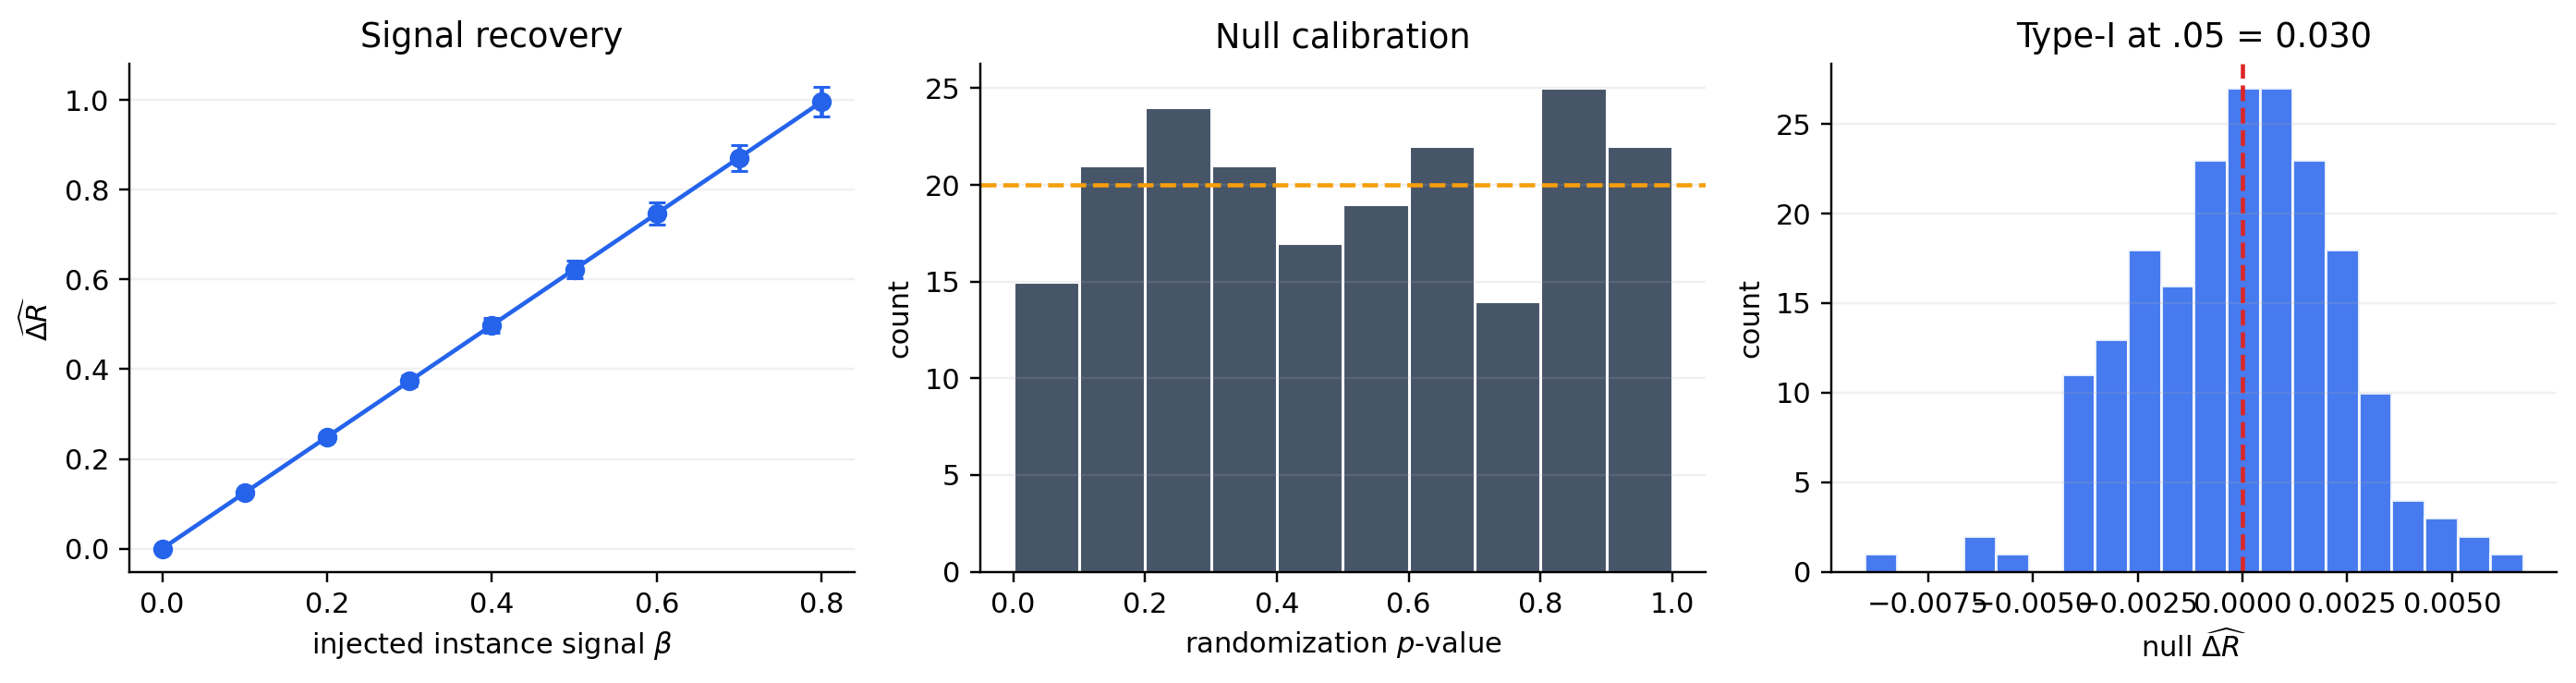
\includegraphics[width=\textwidth]{figures/fig3_new_simulation.png}
\caption{\textbf{Controlled validation.} WAGER recovers injected within-cell signal
monotonically (mean $\pm$ one standard deviation), produces approximately uniform null
randomization $p$-values, and controls type-I error in 200 null runs.}
\label{fig:simulation}
\end{figure*}

\section{Coarsening and unrecorded covariates}\label{app:coarsen}

Appendix~\ref{sec:ablations} reports that replacing the class-pair cell with a coarser
subject-only cell changes the estimated covariance gain. The following result gives that
sensitivity an exact population-level mechanism rather than treating it as an empirical
curiosity.


The first term is the coarse cell's share of the fine-grained covariance gain; the second is
a between-cell covariance, over the finer cells nested inside $\bar c$, between each fine
cell's typical gain at label $y$ and its label-$y$ frequency. It is not sign definite, so
coarsening $\phi$ can inflate or deflate the credited covariance gain, and it vanishes
exactly when either quantity is constant within each coarse cell. This is why the finest
defensible $\phi$ is the conservative default: coarsening adds cross-cell prior structure
into $\Delta R$, while the finer partition's gain is preserved on average through the first
term. The proof is a per-label application of the law of total covariance
(Appendix~\ref{app:proofs}).

\subsection{Sensitivity to an unrecorded confounder}\label{sec:sensitivity}

Read in one direction, Proposition~\ref{prop:coarsen} says what folding a covariate into
$\phi$ does. Read in the other, it quantifies what happens when a relevant covariate is
\emph{never} declared, which is the estimator's main scope limit. Let $Z$ be unrecorded and
let $(\phi,Z)$ be the finer, fully adjusted cell. Applying
Proposition~\ref{prop:coarsen} with $\bar\phi=\phi$ gives, for every declared cell $c$,
\begin{equation}
\Delta R_c(\phi)=\mathbb E\!\left[\Delta R_{(\phi,Z)}\mid\phi=c\right]
+\sum_{y=1}^K\operatorname{Cov}\!\left(\mathbb E[H_X(y)\mid\phi,Z],\,
\Pr(Y=y\mid\phi,Z)\ \middle|\ \phi=c\right),
\label{eq:sensitivity-exact}
\end{equation}
whose first term is what an analyst who could observe $Z$ would report and whose second is
the bias of using $\phi$ alone. The identity is exact but needs $Z$'s joint law with
$(H,Y)$. The following bound replaces that with a judgement about how strongly an unrecorded
variable could plausibly act, in the spirit of \citet{rosenbaum2002observational}.

Proposition~\ref{prop:sensitivity} states that bound and Corollary~\ref{cor:sensitivity-crude}
its data-free form; both are proved in Appendix~\ref{app:proofs}. Because $\bar\rho$ is a
correlation rather than a domain-specific odds ratio, it can be elicited the same way across
benchmarks. Appendix~\ref{app:sensitivity} evaluates both forms on our own estimates, and
the sharp one is the less comfortable: an unrecorded covariate correlated at $0.061$ would
account for the entire covariance gain reported in Appendix~\ref{sec:results}.



\section{Proofs}\label{app:proofs}

\subsection{Proof of Theorem~\ref{thm:population}}
Condition throughout on $C=c$. Expanding over labels gives
\[
\Delta T_c=\sum_y\mathbb E[H_X(y)\ind \{Y=y\}],\qquad
\Delta P_c=\sum_y\mathbb E[H_X(y)]\Pr(Y=y).
\]
Subtracting yields the covariance sum in Eq.~\eqref{eq:population-id}; the first
identity is the definition of $\Delta R_c$. Under the quadratic score,
\[
H_X(y)=2\Delta q_y(X)-\{\lVert q_1(\cdot\mid X)\rVert_2^2-
\lVert q_0(\cdot\mid X)\rVert_2^2\}.
\]
The bracketed term is independent of the label index. Its contribution summed over $y$
is $\operatorname{Cov}(B(X),\sum_y\ind \{Y=y\})=
\operatorname{Cov}(B(X),1)=0$. The remaining terms give Eq.~\eqref{eq:cov-id}. If
$H_X(y)=H_c(y)$ almost surely, every covariance is zero. \qed

\subsection{Proof of Proposition~\ref{prop:transported}}
Condition on $C=c$ and let $Y'\sim p(c)$ be independent of $X$. For the quadratic score
$S_{\rm B}(q,y)=2q_y-\lVert q\rVert^2$,
\begin{equation}
\mathbb E\bigl[S_{\rm B}(q_m,Y')\mid c\bigr]
=2\bigl\langle p(c),\bar q_m(c)\bigr\rangle-\mathbb E\bigl[\lVert q_m\rVert^2\mid c\bigr].
\end{equation}
Decompose the second moment as
$\mathbb E[\lVert q_m\rVert^2\mid c]=\lVert\bar q_m(c)\rVert^2
+\operatorname{tr}\operatorname{Var}(q_m\mid c)$, and complete the square using
$2\langle p,\bar q\rangle-\lVert\bar q\rVert^2=\lVert p\rVert^2-\lVert p-\bar q\rVert^2$:
\begin{equation}
\mathbb E\bigl[S_{\rm B}(q_m,Y')\mid c\bigr]
=\lVert p(c)\rVert^2-\lVert p(c)-\bar q_m(c)\rVert^2
-\operatorname{tr}\operatorname{Var}(q_m\mid c).
\end{equation}
Subtracting the $m=0$ expression from the $m=1$ expression, the $\lVert p(c)\rVert^2$
terms cancel and Eq.~\eqref{eq:transported-composition} follows, since
$\Delta P_c=\mathbb E[S_{\rm B}(q_1,Y')\mid c]-\mathbb E[S_{\rm B}(q_0,Y')\mid c]$ by
definition. \qed

\subsection{Proof of Theorem~\ref{thm:bregman}}
Condition on $C=c$. The proof of Theorem~\ref{thm:population} above establishes
$\Delta R_c=\sum_y\operatorname{Cov}(H_X(y),\ind\{Y=y\}\mid C=c)$ for \emph{any} score
contrast $H$, not only the quadratic one; only the identification of $H_x(y)$ with a
specific functional form is score-dependent. For the Bregman score of
the Bregman score $S_\psi(q,y)=\psi(q)+\langle\nabla\psi(q),e_y-q\rangle$,
\[
H_x(y)=\underbrace{\bigl[\psi(q_1(x))-\psi(q_0(x))\bigr]
-\bigl[\langle\nabla\psi(q_1(x)),q_1(x)\rangle-\langle\nabla\psi(q_0(x)),q_0(x)\rangle\bigr]}_{=:B(x)}
+\;\Delta g_y(x),
\]
writing $q_i(x)$ for $q_i(\cdot\mid x)$, where $B(x)$ collects every term not indexed by
$y$ and $\Delta g_y(x)=\partial_y\psi(q_1(x))-\partial_y\psi(q_0(x))$ is the $y$-indexed
remainder, exactly as in the proof of Theorem~\ref{thm:population} for the quadratic
case. Substituting,
\begin{align*}
\sum_y\operatorname{Cov}(H_X(y),\ind\{Y=y\}\mid c)
&=\operatorname{Cov}\Bigl(B(X),\sum_y\ind\{Y=y\}\ \Big|\ c\Bigr)\\
&\quad+\sum_y\operatorname{Cov}(\Delta g_y(X),\ind\{Y=y\}\mid c).
\end{align*}
The first term is $\operatorname{Cov}(B(X),1\mid c)=0$ since $\sum_y\ind\{Y=y\}=1$
almost surely. The second term is Eq.~\eqref{eq:bregman-cov-id}. \qed

\subsection{Proof of Theorem~\ref{thm:sample}}
Summing the kernel in Eq.~\eqref{eq:kernel} over unordered pairs, every observed term
$H_i(y_i)$ occurs in $n_c-1$ pairs with coefficient $1/2$, while the two crossed terms
together enumerate every ordered pair $H_i(y_j)$, $i\ne j$, with coefficient $1/2$.
Since $\binom{n_c}{2}=n_c(n_c-1)/2$,
\[
\widehat{\Delta R}_c
=\frac1{n_c}\sum_iH_i(y_i)
-\frac1{n_c(n_c-1)}\sum_{i\ne j}H_i(y_j)
=\widehat{\Delta T}_c-\widehat{\Delta P}_c.
\]
This is deterministic. When the cell's examples are i.i.d.\ draws from the cell
population, the average of the symmetric order-two kernel is the standard unbiased
U-statistic for its population expectation \cite{hoeffding1948class}; independence is
used, not merely exchangeability, because $\Delta P_c$ is defined through an independent
label coupling, so $\mathbb E[H_1(Y_2)]=\mathbb E[H_X(Y')]$ requires the two draws to be
independent. \qed

\subsection{Proof of Proposition~\ref{prop:coarsen}}
Fix $y$ and condition throughout on $\bar\phi=\bar c$. The law of total covariance
applied to the pair $(H_X(y),\ind \{Y=y\})$ with the finer conditioning variable $C$
nested inside $\bar c$ gives
\begin{align*}
\operatorname{Cov}\!\left(H_X(y),\ind \{Y=y\}\mid\bar\phi=\bar c\right)
&=\mathbb E\!\left[\operatorname{Cov}(H_X(y),\ind \{Y=y\}\mid C)
   \;\middle|\;\bar\phi=\bar c\right]\\
&\quad+\operatorname{Cov}\!\left(\mathbb E[H_X(y)\mid C],\,
   \Pr(Y=y\mid C)\;\middle|\;\bar\phi=\bar c\right),
\end{align*}
using $\mathbb E[\ind \{Y=y\}\mid C]=\Pr(Y=y\mid C)$. Summing over $y=1,\ldots,K$ and
applying the population identity of Theorem~\ref{thm:population} to the left side (at
$\bar\phi=\bar c$) and to the first term on the right side (at $C=c$, then averaged over
$c$ within $\bar c$) yields Eq.~\eqref{eq:coarsen}. \qed

\subsection{Proof of Proposition~\ref{prop:attenuate}}
Fix a cell $c$ with $n_c\ge2$ and $i\in c$. By definition of the label count,
$\sum_{y=1}^K m_{cy}H_i(y)=\sum_{j\in c}H_i(y_j)=H_i(y_i)+\sum_{j\ne i}H_i(y_j)$, and
Eq.~\eqref{eq:linear} gives $\sum_{j\ne i}H_i(y_j)=(n_c-1)\hat P_i$. Hence
\[
\tilde P_i=\frac1{n_c}\sum_{y}m_{cy}H_i(y)
=\frac{H_i(y_i)+(n_c-1)\hat P_i}{n_c}.
\]
Substituting $H_i(y_i)=\hat P_i+\hat R_i$ gives
$\tilde P_i=\hat P_i+n_c^{-1}\hat R_i$, and $\tilde R_i=H_i(y_i)-\tilde P_i
=\hat R_i-n_c^{-1}\hat R_i=(n_c-1)n_c^{-1}\hat R_i$. Averaging $\tilde R_i$ within cell
$c$ and reweighting by $n_c$ across cells, as in the dataset-level definition of
$\widehat{\Delta Z}$, gives
$\widetilde{\Delta R}=N_*^{-1}\sum_{c}n_c\cdot\frac{n_c-1}{n_c}\widehat{\Delta R}_c
=N_*^{-1}\sum_c(n_c-1)\widehat{\Delta R}_c$. \qed

\subsection{Proof of Proposition~\ref{prop:sensitivity}}
Fix $\phi=c$ throughout and write $a_y=\mathbb E[H_X(y)\mid\phi,Z]$,
$b_y=\Pr(Y=y\mid\phi,Z)$, both random through their dependence on $(\phi,Z)$. Let
$U=(a_y-\mathbb E[a_y\mid c])_{y=1}^K$ and $V=(b_y-\mathbb E[b_y\mid c])_{y=1}^K$ be the
corresponding mean-zero $\mathbb R^K$-valued random vectors conditional on $\phi=c$. The
map $(U,V)\mapsto\mathbb E[\langle U,V\rangle\mid c]=\sum_y\operatorname{Cov}(a_y,b_y\mid c)$
is an inner product on the space of mean-square-integrable $\mathbb R^K$-valued random
variables conditional on $\phi=c$, so by the Cauchy--Schwarz inequality applied to that
inner product,
\[
\Bigl|\sum_{y=1}^K\operatorname{Cov}(a_y,b_y\mid c)\Bigr|
\le\sqrt{\mathbb E[\lVert U\rVert^2\mid c]}\,\sqrt{\mathbb E[\lVert V\rVert^2\mid c]}
=\sqrt{\textstyle\sum_y\operatorname{Var}(a_y\mid c)}\,\sqrt{\textstyle\sum_y\operatorname{Var}(b_y\mid c)}.
\]
By the definition of $\rho$, the left side equals
$|\rho|\sqrt{\sum_y\operatorname{Var}(a_y\mid c)}\sqrt{\sum_y\operatorname{Var}(b_y\mid c)}$
exactly, so this step alone is not yet a bound; two further steps supply one, at two
different levels of conservatism. First, $a_y=\mathbb E[H_X(y)\mid\phi,Z]$ is itself a
conditional expectation of $H_X(y)$ given more information than $\phi=c$ alone, so the
law of total variance gives $\operatorname{Var}(H_X(y)\mid c)=\mathbb
E[\operatorname{Var}(H_X(y)\mid\phi,Z)\mid c]+\operatorname{Var}(a_y\mid c)\ge
\operatorname{Var}(a_y\mid c)$; likewise $b_y=\Pr(Y=y\mid\phi,Z)$ satisfies
$\operatorname{Var}(b_y\mid c)\le\operatorname{Var}(\ind\{Y=y\}\mid c)=p_y(c)(1-p_y(c))$ by
the same argument applied to $\ind\{Y=y\}$ in place of $H_X(y)$. Both bounds hold
termwise, so summing over $y$ and applying the (monotone) square root to each sum
separately gives the observable, per-cell bound
\[
\sqrt{\textstyle\sum_y\operatorname{Var}(a_y\mid c)}\sqrt{\textstyle\sum_y\operatorname{Var}(b_y\mid c)}
\le\sqrt{\textstyle\sum_y\operatorname{Var}(H_X(y)\mid c)}\sqrt{\textstyle\sum_yp_y(c)(1-p_y(c))},
\]
the second inequality of Eq.~\eqref{eq:sensitivity-bound}; this is a bound on a product of
two sums, and does not simplify to a sum of per-label square roots, since Cauchy--Schwarz
runs the other way for that rearrangement. Second, for
Corollary~\ref{cor:sensitivity-crude}, $a_y\in[-M,M]$ as a conditional expectation of a
$[-M,M]$-valued variable, so Popoviciu's inequality gives
$\operatorname{Var}(a_y\mid c)\le M^2$ for every $y$ and hence
$\sum_y\operatorname{Var}(a_y\mid c)\le KM^2$. For the $b_y$ the same argument would give
$\operatorname{Var}(b_y\mid c)\le1/4$ and a total of $K/4$, but that treats the $b_y$ as
$K$ unconstrained quantities in $[0,1]$ when in fact $\sum_yb_y=1$ almost surely. Using
that constraint, $\sum_yb_y^2\le\bigl(\sum_yb_y\bigr)^2=1$ pointwise, while
$\sum_y(\mathbb E b_y)^2\ge K^{-1}\bigl(\sum_y\mathbb E b_y\bigr)^2=1/K$ by
Cauchy--Schwarz, so
\[
\sum_{y=1}^K\operatorname{Var}(b_y\mid c)
=\mathbb E\Bigl[\sum_yb_y^2\Bigr]-\sum_y\bigl(\mathbb E b_y\bigr)^2\le1-\frac1K,
\]
which is Eq.~\eqref{eq:simplex-var} and is strictly smaller than $K/4$ for every $K>2$.
Therefore
\[
\Bigl|\sum_{y=1}^K\operatorname{Cov}(a_y,b_y\mid c)\Bigr|
\le|\rho|\sqrt{KM^2}\sqrt{1-1/K}=|\rho|\,M\sqrt{K-1}.
\]
By Eq.~\eqref{eq:coarsen}, the left side of each display is exactly
$|\Delta R_c(\phi)-\mathbb E[\Delta R_{(\phi,Z)}\mid\phi=c]|$, giving
Eq.~\eqref{eq:sensitivity-bound} and Eq.~\eqref{eq:sensitivity-crude}. \qed

\section{Influence function: estimand and derivation}\label{app:influence}

\paragraph{The estimand under singleton exclusion.} Cells with $n_c=1$ identify no
within-cell counterfactual and are excluded, so the dataset-level statistic targets the
\emph{identified-subpopulation} quantity: writing $\pi_c$ for the cell probabilities,
the target of $\widehat{\Delta R}$ is the $\pi$-weighted mean
$\theta=\sum_c\pi_c\,\Delta R_c/\sum_c\pi_c$ taken over cells that appear with at least
two examples. At finite $N$ the identified set is random; we treat the interval as
conditional on identification and report the identified fraction alongside every
estimate (99.0\% of relations on VG150, 100\% on CIFAR-100-LT), so the gap between the
conditional and full-population targets is bounded by the reported coverage.

\paragraph{Derivation of Eq.~\eqref{eq:influence}.} Fix a cell $c$ and let
$\theta_c=\Delta R_c$ with $g_c(z)=\mathbb E[A(z,Z')\mid Z'\in c]$ the kernel
projection. The classical H\'ajek projection of the order-two U-statistic
$\widehat{\Delta R}_c$ is
\[
\widehat{\Delta R}_c=\theta_c+\frac{2}{n_c}\sum_{i\in c}\bigl(g_c(Z_i)-\theta_c\bigr)
+O_p(n_c^{-1}).
\]
The dataset statistic weights cells by their example counts,
$\widehat{\Delta R}=N_*^{-1}\sum_c n_c\widehat{\Delta R}_c$, and cell membership is
itself random (multinomial over cells), so an example $i$ contributes both through the
within-cell projection and through the between-cell composition term
$\theta_{C_i}-\theta$. Combining the two sources,
\[
\widehat{\Delta R}-\theta
=\frac{1}{N_*}\sum_{i}\Bigl[2\bigl(g_{C_i}(Z_i)-\theta_{C_i}\bigr)
+\bigl(\theta_{C_i}-\theta\bigr)\Bigr]+o_p(N_*^{-1/2}),
\]
where the dataset-level remainder requires one condition beyond the per-cell expansion,
because $C$ per-cell remainders do not aggregate for free. Writing
$C=\#\{c:n_c\ge2\}$ for the number of eligible cells, the weighted sum of the per-cell
degenerate terms is $N_*^{-1}\sum_cn_c\cdot O_p(n_c^{-1})=O_p(C/N_*)$, which is
$o_p(N_*^{-1/2})$ provided
\begin{equation}
C=o\bigl(\sqrt{N_*}\bigr).
\label{eq:cellcount}
\end{equation}
This is what makes the second-order rate $O_p(n_c^{-1})$ rather than $o_p(n_c^{-1/2})$
worth stating: the sharper per-cell rate is what allows a condition on the cell
\emph{count} alone, with no further requirement on individual cell sizes. On VG150,
$C=6{,}346$ against $N_*=227{,}337$, so $C/\sqrt{N_*}\approx13.3$ --- the condition is a
statement about the limit, and at these finite sample sizes it is the coverage simulation
of Section~\ref{sec:simulation}, not Eq.~\eqref{eq:cellcount}, that supports the reported
intervals.
Estimating $g_{C_i}(Z_i)$ by the pair-kernel mean $\bar A_i$, $\theta_c$ by
$\widehat{\Delta R}_c$, and $\theta$ by $\widehat{\Delta R}$ gives the plug-in
influence contribution
$\widehat\psi_i=2(\bar A_i-\widehat{\Delta R}_{c})+(\widehat{\Delta R}_{c}
-\widehat{\Delta R})=2\bar A_i-\widehat{\Delta R}_{c}-\widehat{\Delta R}$, which is
Eq.~\eqref{eq:influence} and has exactly zero sample mean by construction. Its empirical
95\% coverage in a VG-like regime (image-clustered examples, heavy-tailed cell sizes with
a large mass of near-minimum cells) is validated in Section~\ref{sec:simulation}.

\paragraph{Proof of Theorem~\ref{thm:clt}.} The linearization above gives
$\widehat{\Delta R}-\theta=N_*^{-1}\sum_i\psi_i+o_p(N_*^{-1/2})$, under
Eq.~\eqref{eq:cellcount}, for the population
influence contribution $\psi_i=2(g_{C_i}(Z_i)-\theta_{C_i})+(\theta_{C_i}-\theta)$, which
has zero mean by construction and satisfies $|\psi_i|\le C(M)$ for an absolute constant
$C(M)$ depending only on the score bound $M$ in condition (i), since $g_{C_i}$,
$\theta_{C_i}$, and $\theta$ are themselves averages of the bounded kernel
$A_{ij}\in[-2M,2M]$. Because clusters are mutually independent (condition (ii)),
$T_g=\sum_{i\in g}\psi_i$ for $g=1,\dots,G$ are independent, mean-zero random variables
with $|T_g|\le|g|\,C(M)$. Condition (ii)'s finite third moment for cluster sizes and
$\max_g|g|=o(\sqrt G)$ give
$\sum_gE|T_g|^3\le C(M)^3\sum_g\mathbb E|g|^3=O(G)$ while
$\bigl(\sum_g\operatorname{Var}(T_g)\bigr)^{3/2}=\Theta(G^{3/2})$ under condition (iv), so
Lyapunov's ratio $\sum_gE|T_g|^3/(\sum_g\operatorname{Var}(T_g))^{3/2}\to0$; the
Lyapunov condition implies the Lindeberg condition, and the Lindeberg--Feller central
limit theorem for triangular arrays of independent summands
\citep{serfling1980approximation,vandervaart1998asymptotic} gives
$\bigl(\sum_gT_g\bigr)/\sqrt{\sum_g\operatorname{Var}(T_g)}\xrightarrow{d}\mathcal N(0,1)$.
Condition (iii) makes $N_*/\sum_g\operatorname{Var}(T_g)\to1/\sigma^2$ in probability by
definition of $\sigma^2$, and the $o_p(N_*^{-1/2})$ remainder is asymptotically
negligible after multiplying by $\sqrt{N_*}$, so
$\sqrt{N_*}(\widehat{\Delta R}-\theta)\xrightarrow{d}\mathcal N(0,\sigma^2)$ by Slutsky's
theorem. For the variance estimator, $\widehat{\Delta R}\to_p\theta$ by the weak law of
large numbers across the diverging number of identified examples, and
$\widehat{\Delta R}_c\to_p\Delta R_c$ for each eligible cell by the weak law of large
numbers applied within that cell -- this is where condition (iv) is used, and it is not
implied by anything aggregate: (iv) guarantees $n_c\to\infty$ almost surely for every cell
in the fixed, finite support of $\phi$, which is what a within-cell WLLN requires, whereas
a condition on the total identified count bounds no individual cell's size. So $\widehat\psi_i\to_p\psi_i$ pointwise, and
$\widehat\sigma^2$ -- a sum of squares of cluster-aggregated $\widehat\psi_i$, normalized
by $N_*$ and $G$ -- is a continuous functional of these consistent plug-ins, hence
$\widehat\sigma^2\to_p\sigma^2$ by the continuous mapping theorem. \qed

\paragraph{Efficient computation.} The implementation does not instantiate all pairs. In addition to Eq.~\eqref{eq:linear},
let $G_c(y)=\sum_{j\in c}H_j(y)$ and $O_c=\sum_{j\in c}H_j(y_j)$. The pair-kernel mean
for observation $i$ is
\[
\bar A_i=\frac12\left[
H_i(y_i)+\frac{O_c-H_i(y_i)}{n_c-1}
-P_i-\frac{G_c(y_i)-H_i(y_i)}{n_c-1}
\right].
\]
Therefore both the point estimate and H\'ajek projection require only label counts,
column sums, and matrix--vector products inside each cell. For image clusters $g$, the
implemented variance is
\[
\widehat{\operatorname{Var}}(\widehat{\Delta R})
=\frac{G}{G-1}\frac1{N_*^2}\sum_{g=1}^G
\left(\sum_{i\in g}\widehat\psi_i\right)^2,
\]
where $G$ is the number of images and $\widehat\psi_i$ is
Eq.~\eqref{eq:influence}. We use a normal critical value; with 27,955 image clusters,
small-$G$ corrections are immaterial.

\section{Randomization algorithm}\label{app:random}

For each cell, sort examples once and index them $0,\ldots,n_c-1$. Randomization $b$
draws $o_c^{(b)}$ uniformly from this index set and maps label position $r$ to
$(r+o_c^{(b)})\bmod n_c$. Independent offsets across cells define an element of the
product of cyclic groups. The cell label histogram is unchanged, so
$\sum_y m_{cy}H_i(y)$ in Eq.~\eqref{eq:linear} is precomputed; only the assigned label
lookup changes. One randomization is $O(N)$ after the $O(NK)$ setup. The plus-one Monte
Carlo correction includes the observed assignment and prevents zero $p$-values.

\begin{algorithm}[t]
\caption{WAGER gain decomposition}\label{alg:wager}
\begin{algorithmic}[1]
\Require frozen $q_1,q_0$; labels $y$; cells $\phi$; proper score $S$
\Ensure $\widehat{\Delta T},\widehat{\Delta P},\widehat{\Delta R}$ and uncertainty
\State $H_i(k)\gets S(q_{1i},k)-S(q_{0i},k)$ for all $i,k$
\For{each cell $c$ with $n_c\ge2$}
  \State count labels $m_{c1},\ldots,m_{cK}$
  \For{each $i\in c$}
    \State $P_i\gets(\sum_k m_{ck}H_i(k)-H_i(y_i))/(n_c-1)$
    \State $R_i\gets H_i(y_i)-P_i$
  \EndFor
\EndFor
\State $\widehat{\Delta T}\gets\operatorname{mean}H_i(y_i)$;
$\widehat{\Delta P}\gets\operatorname{mean}P_i$;
$\widehat{\Delta R}\gets\operatorname{mean}R_i$
\State compute image-clustered H\'ajek interval and cell-shift randomization $p$
\end{algorithmic}
\end{algorithm}

\section{Implementation and reproducibility}\label{app:implementation}

The NumPy implementation is in \texttt{wager/antisymmetric.py}. The primary routine
\texttt{decompose\_gain} validates probability matrices, forms score contrasts, excludes
singleton cells, computes all three components, verifies the identity numerically, and
returns per-instance transported/covariance values plus intervals. The Visual Genome
driver is \texttt{experiments/\allowbreak run\_sgg\_wager.py}; controlled validation and sensitivity
checks are in \texttt{experiments/\allowbreak antisymmetric\_simulation.py} and
\texttt{experiments/\allowbreak antisymmetric\_ablations.py}. All random seeds are fixed. Unit tests
cover the decomposition identity, quadratic covariance identity, cell-constant null,
singleton reporting, cluster inference, randomization power, and log-score path, plus
direct numerical checks of Propositions~\ref{prop:attenuate} and~\ref{prop:coarsen}
(the latter against an explicit discrete population with exact expectations, independent
of the estimator's own code path), Corollary~\ref{cor:bregman}'s log-score covariance
identity, Corollary~\ref{cor:dm}'s equivalence to the (unclustered) Diebold--Mariano
statistic at a trivial grouping variable, and Proposition~\ref{prop:sensitivity}'s bound
ordering (exact bias $\le$ tight, per-cell bound $\le$ crude, data-free bound) on a second
explicit discrete population with a known omitted confounder. The covariance-identity
cross-check quoted in
Section~\ref{app:lt} is reproduced by
\texttt{experiments/\allowbreak cifar\_covariance\_check.py}; the calibration-matched
protocol and the prior-matching experiment are
\texttt{experiments/\allowbreak cifar\_recalibration\_control.py} and
\texttt{experiments/\allowbreak vg\_prior\_consequence.py}. Table~\ref{tab:sensitivity-numeric}'s
free-bound rows are reproduced by \texttt{experiments/\allowbreak
sensitivity\_bound\_check.py} and its sharp rows, including the robustness value
$\rho^\dagger$ of Eq.~\eqref{eq:robustness-value}, by
\texttt{experiments/\allowbreak sensitivity\_analysis.py}; the evaluation of
Corollary~\ref{cor:sensitivity-crude} is
\texttt{experiments/\allowbreak sensitivity\_bound\_check.py}, which recomputes the crude
bound directly from the committed \texttt{antisymmetric\_ablations.json} rather than
re-running the decomposition; \texttt{experiments/\allowbreak sensitivity\_analysis.py}
computes Proposition~\ref{prop:sensitivity}'s tighter, per-cell form from per-instance
arrays (Section~\ref{app:compute}).

\paragraph{Full-data VG predictors (Sections~\ref{app:vgmain-full}--\ref{sec:ablations}).}
FREQ uses add-one smoothing over the $50$ predicates within each training class pair,
backing off to the subject-marginal and then the global predicate histogram for pairs
unseen in training. The MLPs consume fixed random class embeddings
($32$ dimensions per class, seed $0$, concatenated for subject and object) on
standardized features and train with AdamW (learning rate $10^{-3}$, weight decay
$10^{-5}$, batch size $4096$): MLP-CLASS with hidden sizes $(256,128)$ for $12$ epochs,
MLP-SPATIAL with $(256,128)$ for $15$ epochs, and MLP-SPATIAL+ with $(512,256,128)$ for
$20$ epochs -- the ``+'' variant differs in both width and schedule, as noted in
Section~\ref{sec:data}.

\paragraph{Data availability.} The repository ships the estimator, every driver script,
and the cached results files that every printed number traces to
(\texttt{results/*.json}). The cached per-relation probability arrays that the drivers
consume (\texttt{sgg\_dists.npz}, \texttt{vg\_visual\_models.npz},
\texttt{cifar\_lt\_results.npz}) are regenerable from the committed training scripts
with fixed seeds and are archived alongside the code release, so exact reproduction
does not require retraining.

\subsection{Compute environment for Sections~\ref{app:vgvisual-full}--\ref{app:lt}}\label{app:compute}

Model training and feature extraction for both new experiments ran on a single NVIDIA
T4 (15\,GB) GPU. The WAGER decomposition itself is pure NumPy and requires no
accelerator: it consumes the resulting cached probability arrays, as in
Section~\ref{sec:data}. All Python code runs under a pinned environment (Python 3.13).

\paragraph{Matched-subsample models (Section~\ref{sec:vgvisual}).} The three compared
predictors share a fixed, seeded ($\text{seed}=0$) subsample of $100{,}000$ of the
$532{,}987$ training relations, drawn without replacement uniformly at the relation
level (not the image level); the full $229{,}605$-relation test split is always used for
evaluation. All three use the identical head and optimizer -- AdamW, learning rate
$10^{-3}$, weight decay $10^{-5}$, 15 epochs, batch size 4096, hidden sizes
$(256,128)$, on standardized features -- so they differ only in their input features.

Subject/object crops are taken from the annotated boxes and CLIP-preprocessed (bicubic
resize to $224\times224$ with CLIP's published normalization constants); a crop with no
valid overlap with the image falls back to a blank crop rather than being dropped, so
every relation contributes a feature row. CLIP runs in half precision with a batch size
of $512$ crops and is never fine-tuned. Two implementation details are worth recording.
First, the pretrained OpenAI weights were trained with the QuickGELU activation, so the
encoder must be instantiated as \texttt{ViT-B-32-quickgelu}; loading the same weights
under the plain \texttt{ViT-B-32} configuration silently substitutes a standard GELU and
degrades every embedding. Second, because an annotated object box participates in
several relations, crops are deduplicated by (image, box) before encoding and gathered
afterwards: the $659{,}210$ crops implied by the audited relations collapse to
$422{,}143$ unique ones, removing $36.0\%$ of the encoder work without changing any
feature. Only the images referenced by those relations are retrieved, individually rather
than through the two bulk archives; of the $71{,}990$ required, three were unavailable
upstream and fall back to a blank crop.

\paragraph{ResNet-32 triple (Section~\ref{app:lt}).} CIFAR-100-LT uses the standard
exponential-profile construction of \citet{cui2019classbalanced} at imbalance ratio
$100$: class $c$ (zero-indexed, $0,\ldots,99$) keeps
$n_c=\lfloor 500\cdot\mu^{c}\rfloor$ training images, where
$\mu=100^{-1/99}$, so class $0$ keeps all $500$ images and class $99$ keeps $5$; the
balanced $10{,}000$-image test split is untouched. All three models are a from-scratch,
randomly initialized CIFAR ResNet-32 (three stages of five basic residual blocks,
$16/32/64$ channels) trained for $80$ epochs with SGD (momentum $0.9$, Nesterov,
weight decay $2\times10^{-4}$), batch size $128$, standard crop-and-flip augmentation,
and a cosine learning-rate schedule (peak $0.1$, five-epoch linear warmup). The only
difference between the runs is the per-example loss weight. CE uses uniform weights
throughout. CB applies the effective-number class-balanced weight
$w_c\propto(1-\beta)/(1-\beta^{n_c})$ with $\beta=0.9999$, renormalized to average to
one across classes, from initialization. DRW trains with uniform weights until epoch
$60$ and switches to exactly the CB weights for the final twenty epochs
\citep{cao2019learning}; no other hyperparameter changes at the switch. The robustness
matrix of Table~\ref{tab:cifar-robust} repeats this recipe verbatim at seeds $1$ and $2$
(ratio $100$) and at ratios $10$ and $50$ (seed $0$), re-drawing the long-tailed subset
with the configuration's own seed and initializing all three arms of a configuration
identically (\texttt{experiments/colab\_cifar\_multiseed.py}). The post-hoc LA arm is not
trained: it rescales the baseline's test probabilities by the inverse training class
prior, $q_{\mathrm{LA}}(y\mid x)\propto q_{\mathrm{CE}}(y\mid x)/\pi_{\mathrm{train}}(y)$,
renormalized.

\section{Sensitivity bounds on the reported estimates}\label{app:sensitivity}

\paragraph{What the bound says about this paper's own estimates.}
Table~\ref{tab:sensitivity-numeric} reports both forms of the bound on the Visual Genome
pair of Section~\ref{sec:results}, together with the coarsening from the class-pair to
the subject-only cell, which instantiates Eq.~\eqref{eq:coarsen} exactly with
$Z=$ object class. The free bound is directionally correct and, at $K=50$, still
$1{,}887$ times the actual coarsening bias, so any $\bar\rho$ an analyst would plausibly
declare certifies a limit far above what is observed. That looseness is a property of a
worst-case inequality applied to label probabilities that concentrate away from the
extremes at which it binds, not a defect of this dataset --- but it also means the free
bound cannot support a claim about whether any particular reported $\widehat{\Delta R}$
would survive confounding.

The sharp per-cell form of Eq.~\eqref{eq:sensitivity-bound}, which replaces the
worst-case sums by the cell's own $\sum_y\operatorname{Var}(H_X(y)\mid c)$ and
$\sum_yp_y(c)(1-p_y(c))$, can support such a claim, and it is less reassuring than the
free bound. Computed by \texttt{experiments/sensitivity\_analysis.py} from per-instance
arrays for the same pair, it gives $B=0.23284$ at $\bar\rho=1$, so the
\emph{robustness value} --- the smallest aggregate correlation at which the bound reaches
the estimate --- is
\begin{equation}
\rho^\dagger=\frac{\bigl|\widehat{\Delta R}\bigr|}{B}
=\frac{0.01427}{0.23284}=0.06127 .
\label{eq:robustness-value}
\end{equation}
An unrecorded covariate whose aggregate correlation with the within-cell gain and the
within-cell label distribution reaches $0.061$ is enough to account for the whole of that
$\widehat{\Delta R}$. At the $\bar\rho=0.1$ that this section suggests as a plausible
elicited value, the sharp bound is $0.02328$, which \emph{exceeds} the estimate. We
therefore do not claim that a confounder would have to be implausibly strong to explain
these Visual Genome gains away; on this evidence a modest one would suffice, and the
reader should treat Section~\ref{sec:results}'s covariance gains as conditional on the
declared $\phi$ being close to complete. The flagship audit of
Section~\ref{sec:sggaudit} is not exposed in the same way, because its reported
$\widehat{\Delta R}$ is indistinguishable from zero and a sensitivity bound on a null
result changes nothing about it.

\begin{table}[t]
\centering
\caption{Both forms of the Proposition~\ref{prop:sensitivity} bound on the
MLP-SPATIAL vs.\ MLP-CLASS pair, and the coarsening already reported in
Table~\ref{tab:sensitivity} ($K=50$, $M=2$ for the quadratic score). The empirical bias
is the law-of-total-expectation aggregate of Eq.~\eqref{eq:coarsen}'s covariance
term across all subject-only cells.
\texttt{experiments/sensitivity\_bound\_check.py} reproduces the free-bound rows from the
committed ablation results and \texttt{experiments/sensitivity\_analysis.py} the sharp
rows from per-instance arrays.}
\label{tab:sensitivity-numeric}
\begin{tabular}{lr}
\toprule
Quantity & Value \\
\midrule
$\widehat{\Delta R}$, $\phi=$ subject-only & $0.02181$ \\
$\widehat{\Delta R}$, $\phi=$ class-pair & $0.01439$ \\
Empirical coarsening bias & $0.00742$ \\
\midrule
Free bound, $M\sqrt{K-1}$, at $\bar\rho=1$ & $14.00$ \\
Minimum $\bar\rho$ for the free bound to reach the bias & $0.00053$ \\
\midrule
Sharp bound $B$ at $\bar\rho=1$ & $0.23284$ \\
Sharp bound at $\bar\rho=0.1$ & $0.02328$ \\
Robustness value $\rho^\dagger$ & $0.06127$ \\
\bottomrule
\end{tabular}
\end{table}

\section{Conditions for the limit theorem}\label{app:clt}

Two things about condition (iv) deserve saying plainly rather than in a footnote. It is
what licenses treating the per-cell plug-ins $\widehat{\Delta R}_c$ as consistent for
$\Delta R_c$ in the variance argument, and a cell's size is not controlled by the
aggregate identified count, so this needs its own divergence requirement. But it also
forces every cell to be eventually identified, hence $N_*/N\to1$: an earlier version of
this theorem additionally assumed an identified fraction converging to some
$\kappa\in(0,1]$, which condition (iv) makes vacuous, and under which the
identified-subpopulation estimand $\theta$ would in any case coincide with the
unconditional target. We have therefore dropped that assumption rather than state two
conditions that cannot both bind. The price is that the theorem does not describe the
regime the paper's own applications sit in, where $\theta$ is a random, $N$-dependent
target because coverage is short of one ($99.0\%$ on VG150, $98.9\%$ in
Section~\ref{sec:sggaudit}). What the theorem licenses is the interval's form and its
variance estimator; what licenses reading the reported intervals at finite $N$ is the
coverage simulation of Section~\ref{sec:simulation}, and Section~\ref{sec:discussion}
states the gap between the two rather than eliding it.

The proof (Section~\ref{app:proofs}) combines the exact linearization of
Section~\ref{app:influence} with a Lindeberg--Feller central limit theorem for the
independent-across-cluster sum of mean-zero, uniformly bounded terms
\citep{serfling1980approximation,vandervaart1998asymptotic}; boundedness (i) makes the
Lindeberg condition automatic given (ii), and consistency of $\widehat\sigma^2$ follows
from the weak law of large numbers applied to each plug-in $\widehat{\Delta R}_c,
\widehat{\Delta R}$ together with continuity of the variance functional. One step needs
more care than that section's per-cell statement supplies: a per-cell H\'ajek remainder of
order $o_p(n_c^{-1/2})$ does not aggregate to $o_p(N_*^{-1/2})$ at the dataset level when
the number of cells grows, since summing $C$ such remainders admits a $\sqrt C$ inflation.
The repair does not need a new condition on cell sizes, only that the cell count be
negligible relative to the identified sample, $\#\{c:n_c\ge2\}=o(N_*)$: the second-order
degenerate term of a two-sample U-statistic is $O_p(n_c^{-1})$ rather than
$o_p(n_c^{-1/2})$, and $\sum_c n_c\cdot O_p(n_c^{-1})=O_p(C)=o_p(N_*)$ gives the
dataset-level rate directly. We state that condition explicitly; on VG150 it holds
comfortably ($C=6{,}346$ against $N_*=227{,}337$). Condition (ii) is what rules out a single cluster dominating the
sum -- an image contributing a positive fraction of all relations, for instance -- and
is a standard requirement for cluster-robust inference generally, not specific to this
estimator. This theorem licenses reading the image-clustered intervals reported
throughout Section~\ref{sec:exp} as asymptotically valid in the idealized regime where
every eligible cell's size grows without bound. That regime is not attained in-sample:
VG150's eligible cells are heavy-tailed, and $2{,}286$ of the $6{,}346$ eligible
class-pair cells hold fewer than five examples (Table~\ref{tab:sensitivity}). The
proportion is smaller than earlier drafts of this paper asserted --- those cells carry
$2.7\%$ of identified relations, and the median eligible cell holds appreciably more than
the minimum --- but a third of the cells still sit where condition (iv)'s divergence is
plainly hypothetical. The reported $94.0\%$ empirical coverage against a nominal $95\%$
(Section~\ref{sec:simulation}), not this theorem directly, is therefore the evidence that
the interval remains a good approximation well short of the idealization.

\section{Choice of the grouping variable}\label{app:partition}

\paragraph{Fineness is not a total order, and the guidance needs that qualification.}
The advice to prefer the finest defensible $\phi$ is sound against \emph{coarsening},
which is what Proposition~\ref{prop:coarsen} governs. It gives no guidance at all between
two partitions of the same granularity, neither of which coarsens the other --- and there
the estimand can differ without limit. Four cases suffice. Take two labels, $q_0$
uninformative at $(\tfrac12,\tfrac12)$, and a new model that is confidently right on all
four: $q_1=(0.9,0.1)$ on the two cases labelled $1$ and $(0.1,0.9)$ on the two labelled
$2$. The total gain is $\widehat{\Delta T}=+0.480$ under every partition, and every
partition below is fully identified at $100\%$ coverage:
\begin{center}
\begin{tabular}{@{}lccr@{}}
\toprule
declared $\phi$ & cells & $\widehat{\Delta P}$ & $\widehat{\Delta R}$ \\
\midrule
$\{1,3\},\{2,4\}$ (labels differ within each cell) & $2\times2$ & $-1.120$ & $+1.600$ \\
$\{1,2,3,4\}$ (one cell)                           & $1\times4$ & $-0.587$ & $+1.067$ \\
$\{1,2\},\{3,4\}$ (labels agree within each cell)  & $2\times2$ & $+0.480$ & $\phantom{+}0.000$ \\
\bottomrule
\end{tabular}
\end{center}
The first and third partitions are equally fine, both fully identified, and they disagree
about whether this model pair's improvement is entirely case-level or entirely
transported. The third is the degenerate case the paper already warns about --- grouping
by something that determines the label leaves each cell label-homogeneous and drives
$\widehat{\Delta R}$ to zero algebraically --- but the warning was previously attached to
the choice $\phi=Y$, and the point here is more general and less comfortable: any $\phi$
correlated with the label inside a cell partially degenerates the estimand, ``finest
defensible'' cannot detect it, and Proposition~\ref{prop:coarsen} is silent because
neither partition is a coarsening of the other. What the analyst actually needs to
declare, and what we recommend reporting alongside $\phi$, is the within-cell label
heterogeneity that remains: a partition whose cells are nearly label-homogeneous cannot
identify much of anything, and the coverage statistic does not reveal it. This is a
limitation of the construction rather than of any application of it, and we do not have a
procedure that resolves it.

\paragraph{A recalibration-invariant alternative, and what it would cost.}
Because $\Delta R$ is a covariance between forecast values, its sensitivity to
recalibration is structural rather than incidental, and a reader may reasonably ask why we
do not use a rank-based within-cell contrast instead --- a within-cell paired AUC
difference, say, for which \citet{delong1988comparing} already supply the
correlated-U-statistic variance. Such a quantity would be invariant to any monotone
rescaling of either model and would dissolve the confound this paper spends a protocol on.
We think the trade is worth stating and is not obviously in our favour on every axis.
What a rank-based contrast gives up is the exact identity: it is not a component of the
score difference, so it cannot be added to anything to recover $\Delta T$, and a benchmark
reporting it learns how the models rank cases but not how the reported score gain
decomposes. The construction here buys exact additivity with respect to a declared proper
score, and pays for it with scale dependence. A rank-based diagnostic is the natural
companion rather than a competitor, and reporting both --- one exact and scale-dependent,
one invariant and non-additive --- is what we would now recommend to a benchmark that
could choose.

% --- statements relocated from the method section for length ---


Earlier versions of this corollary bounded $\sum_y\operatorname{Var}(b_y\mid c)$ by
Popoviciu's inequality applied label by label, giving $K/4$ and hence $|\rho|KM/2$. That
discards Eq.~\eqref{eq:simplex-var}: the $b_y$ are not $K$ unconstrained quantities in
$[0,1]$ but a point on the simplex, and $K/4$ is unattainable for $K>2$. At VG150's
$K=50$ and $M=2$ the corrected free bound is $14.00|\rho|$ rather than $50.00|\rho|$, a
factor of $3.57$.

An analyst willing to bound $|\rho|\le\bar\rho$ -- how strongly an unrecorded variable
could jointly move a model's within-cell score gain and the within-cell label
distribution -- obtains a numeric limit on how far $\widehat{\Delta R}_c$ can be from
what a fully adjusted audit would find, without observing or modeling $Z$, in the spirit
of \citet{rosenbaum2002observational} and recent partial-correlation sensitivity models
for unmeasured confounding \citep{cinelli2020making}.
Because $\bar\rho$ is a correlation rather than a domain-specific odds or risk ratio, it
can be elicited the same way across benchmarks.

Both forms of the bound are evaluated on this paper's own Visual Genome estimates in
Section~\ref{app:sensitivity}. The short version is that the free bound is directionally
correct but far too loose to certify anything, while the sharp per-cell form is
\emph{less} reassuring than the free one: an unrecorded covariate whose aggregate
correlation with both channels reaches $0.061$ would account for the entire covariance gain
reported in Section~\ref{sec:results}. We therefore do not claim those gains are robust to
confounding, and Section~\ref{sec:sggaudit}'s audit is unaffected only because its estimate
is already indistinguishable from zero.


Section~\ref{app:clt} discusses what condition (iv) costs --- it forces every cell to be
eventually identified, so the theorem does not describe the finite-sample regime our own
applications sit in --- and states the additional condition on the number of cells that the
dataset-level remainder requires. What licenses reading the reported intervals at finite $N$
is the coverage simulation of Section~\ref{sec:simulation}, not this theorem.

\section{Terminology}\label{app:terms}

\begin{table}[t]
\centering
\small
\caption{The paper's vocabulary, and what it corresponds to in standard terms.}
\label{tab:terms}
\begin{tabular}{@{}p{0.24\textwidth}p{0.30\textwidth}p{0.38\textwidth}@{}}
\toprule
Term used here & Standard counterpart & Meaning \\
\midrule
grouping variable $\phi$ &
stratifying / conditioning variable &
a discrete function of the input, declared before the audit, whose levels the labels
depend on \\
cell $c$ &
level of $\phi$; stratum &
the set of test cases sharing one value of $\phi$ \\
label transport &
within-stratum relabelling; permutation within blocks &
replacing a case's label with another case's label from the same cell \\
total gain $\Delta T$ &
paired score differential &
the observed mean score of the new model minus that of the old \\
transported gain $\Delta P$ &
no exact counterpart; a mean-forecast-fit term minus a dispersion term
(Proposition~\ref{prop:transported}), \emph{not} a measure of prior fit &
the part of $\Delta T$ that survives label transport \\
within-group covariance gain $\Delta R$ &
the covariance term of a covariance rearrangement of a proper score
\citep{yates1982external}; twice a classical resolution difference \emph{only} under
within-cell calibration &
the part destroyed by transport; a within-cell prediction--label covariance \\
coverage &
identified fraction &
share of test cases in cells of size $\ge2$, the only cells in which $\Delta R$ is
identified \\
calibration-matched &
temperature-scaled on held-out data &
both models rescaled to comparable confidence before the audit \\
\bottomrule
\end{tabular}
\end{table}

\section{Why the transported gain is not prior fit}\label{app:transported}

Proposition~\ref{prop:transported} splits $\Delta P_c$ into two brackets, and only the
first is prior fit: it is positive exactly when the new model's average
within-cell forecast sits closer to the cell's label frequencies. The second has nothing to
do with the prior. It rewards the new model for making \emph{less} dispersed predictions
inside the cell, at a fixed mean forecast, so $\Delta P$ can be large and positive when
neither model's prior fit has changed at all. One cell suffices: with two labels and
frequencies $(\tfrac12,\tfrac12)$, let $q_0$ alternate between $(1,0)$ and $(0,1)$ in a
pattern uncorrelated with the label and let $q_1$ predict $(\tfrac12,\tfrac12)$ throughout.
Both mean forecasts equal the cell frequencies exactly, so the first bracket is zero, and the
whole observed gain of $\tfrac12$ is transported, produced entirely by the collapse in
dispersion. The channel is therefore the reliability-and-sharpness channel of the classical
partition, not a prior-fitting channel, which is why we name it for the operation. Two
consequences: a claim that some gain is ``mostly prior-fitting'' does not follow from a large
$\widehat{\Delta P}$ alone, and Eq.~\eqref{eq:transported-composition} explains why
confidence matching moves $\widehat{\Delta P}$ so sharply, since a temperature change is
almost purely a change in dispersion.


\section{Further empirical studies}\label{app:studies}

This section reports the two studies summarized in Section~\ref{sec:further} and the
granularity, score and cell-size sensitivity analyses referred to there. Each applies the
estimator of Section~\ref{sec:method} without modification; only the declared grouping
variable $\phi$ changes.

\subsection{Controlled predictors on VG150 in full}\label{app:vgmain-full}

We work with Visual Genome \cite{krishna2017visual} in the PredCls regime
\cite{xu2017scene}, where ground-truth boxes and object labels are supplied and
the model has only to predict one of 50 predicate labels for each ordered object pair.
The predictors of this section are audited on a VG150-\emph{style} dataset we build
directly from the released relationship annotations: the 150 most frequent object
classes and 50 most frequent predicates form the vocabulary, and images are split
$70/30$ into a pool for fitting the compared predictors and a pool on which the audit
runs. We use this reconstruction rather than the canonical VG150 release because these
predictors are trained here from annotations alone; Section~\ref{sec:sggaudit} audits
\emph{released third-party checkpoints} on the canonical split itself, so both settings
appear in the paper and neither is asked to stand for the other. The reconstruction
provides 532,987 training and 229,605 test relations, drawn from 65,228 and 27,955
images respectively, and the cell throughout is
$\phi=(\text{subject class},\text{object class})$, two real examples of which appear in
Figure~\ref{fig:samples}. Of the 8,614 cells present in the test split, 6,346 contain at
least two relations and are therefore identified; the remaining 2,268 are singletons,
which WAGER excludes and reports rather than smoothing over, leaving 227,337 relations
(99.0\%) under audit.

The five predictors are deliberately constructed so that each exposes a different kind
of information. FREQ is the training-count distribution conditioned on the class pair,
with add-one smoothing and a subject-marginal and then global backoff for class pairs
unseen in training; FREQ+OVERLAP adds to it a single binary box-overlap indicator.
MLP-CLASS consumes fixed subject and object class embeddings, which makes it a function
of $\phi$ alone; MLP-SPATIAL extends those embeddings with 12 normalized box-geometry
features covering relative centre, scale, aspect, intersection, containment and IoU,
while MLP-SPATIAL+ both widens the network and trains longer (Section~\ref{app:implementation} lists every architecture and schedule), so its increment over
MLP-SPATIAL reflects capacity and optimization jointly rather than capacity alone. Each
is trained once on the training split, and WAGER thereafter consumes nothing but their
cached test distributions, scored quadratically with image-clustered intervals and 499
within-cell cyclic randomizations, whose smallest attainable $p$-value is
$1/500=.002$; table entries of $.002$ are at this granularity floor and should be read
as $p\le.002$. With confidence intervals as the primary uncertainty statement and every
significant effect many standard errors from zero, we do not additionally adjust the
diagnostic $p$-values for the number of reported comparisons.

\begin{figure*}[t]
\centering
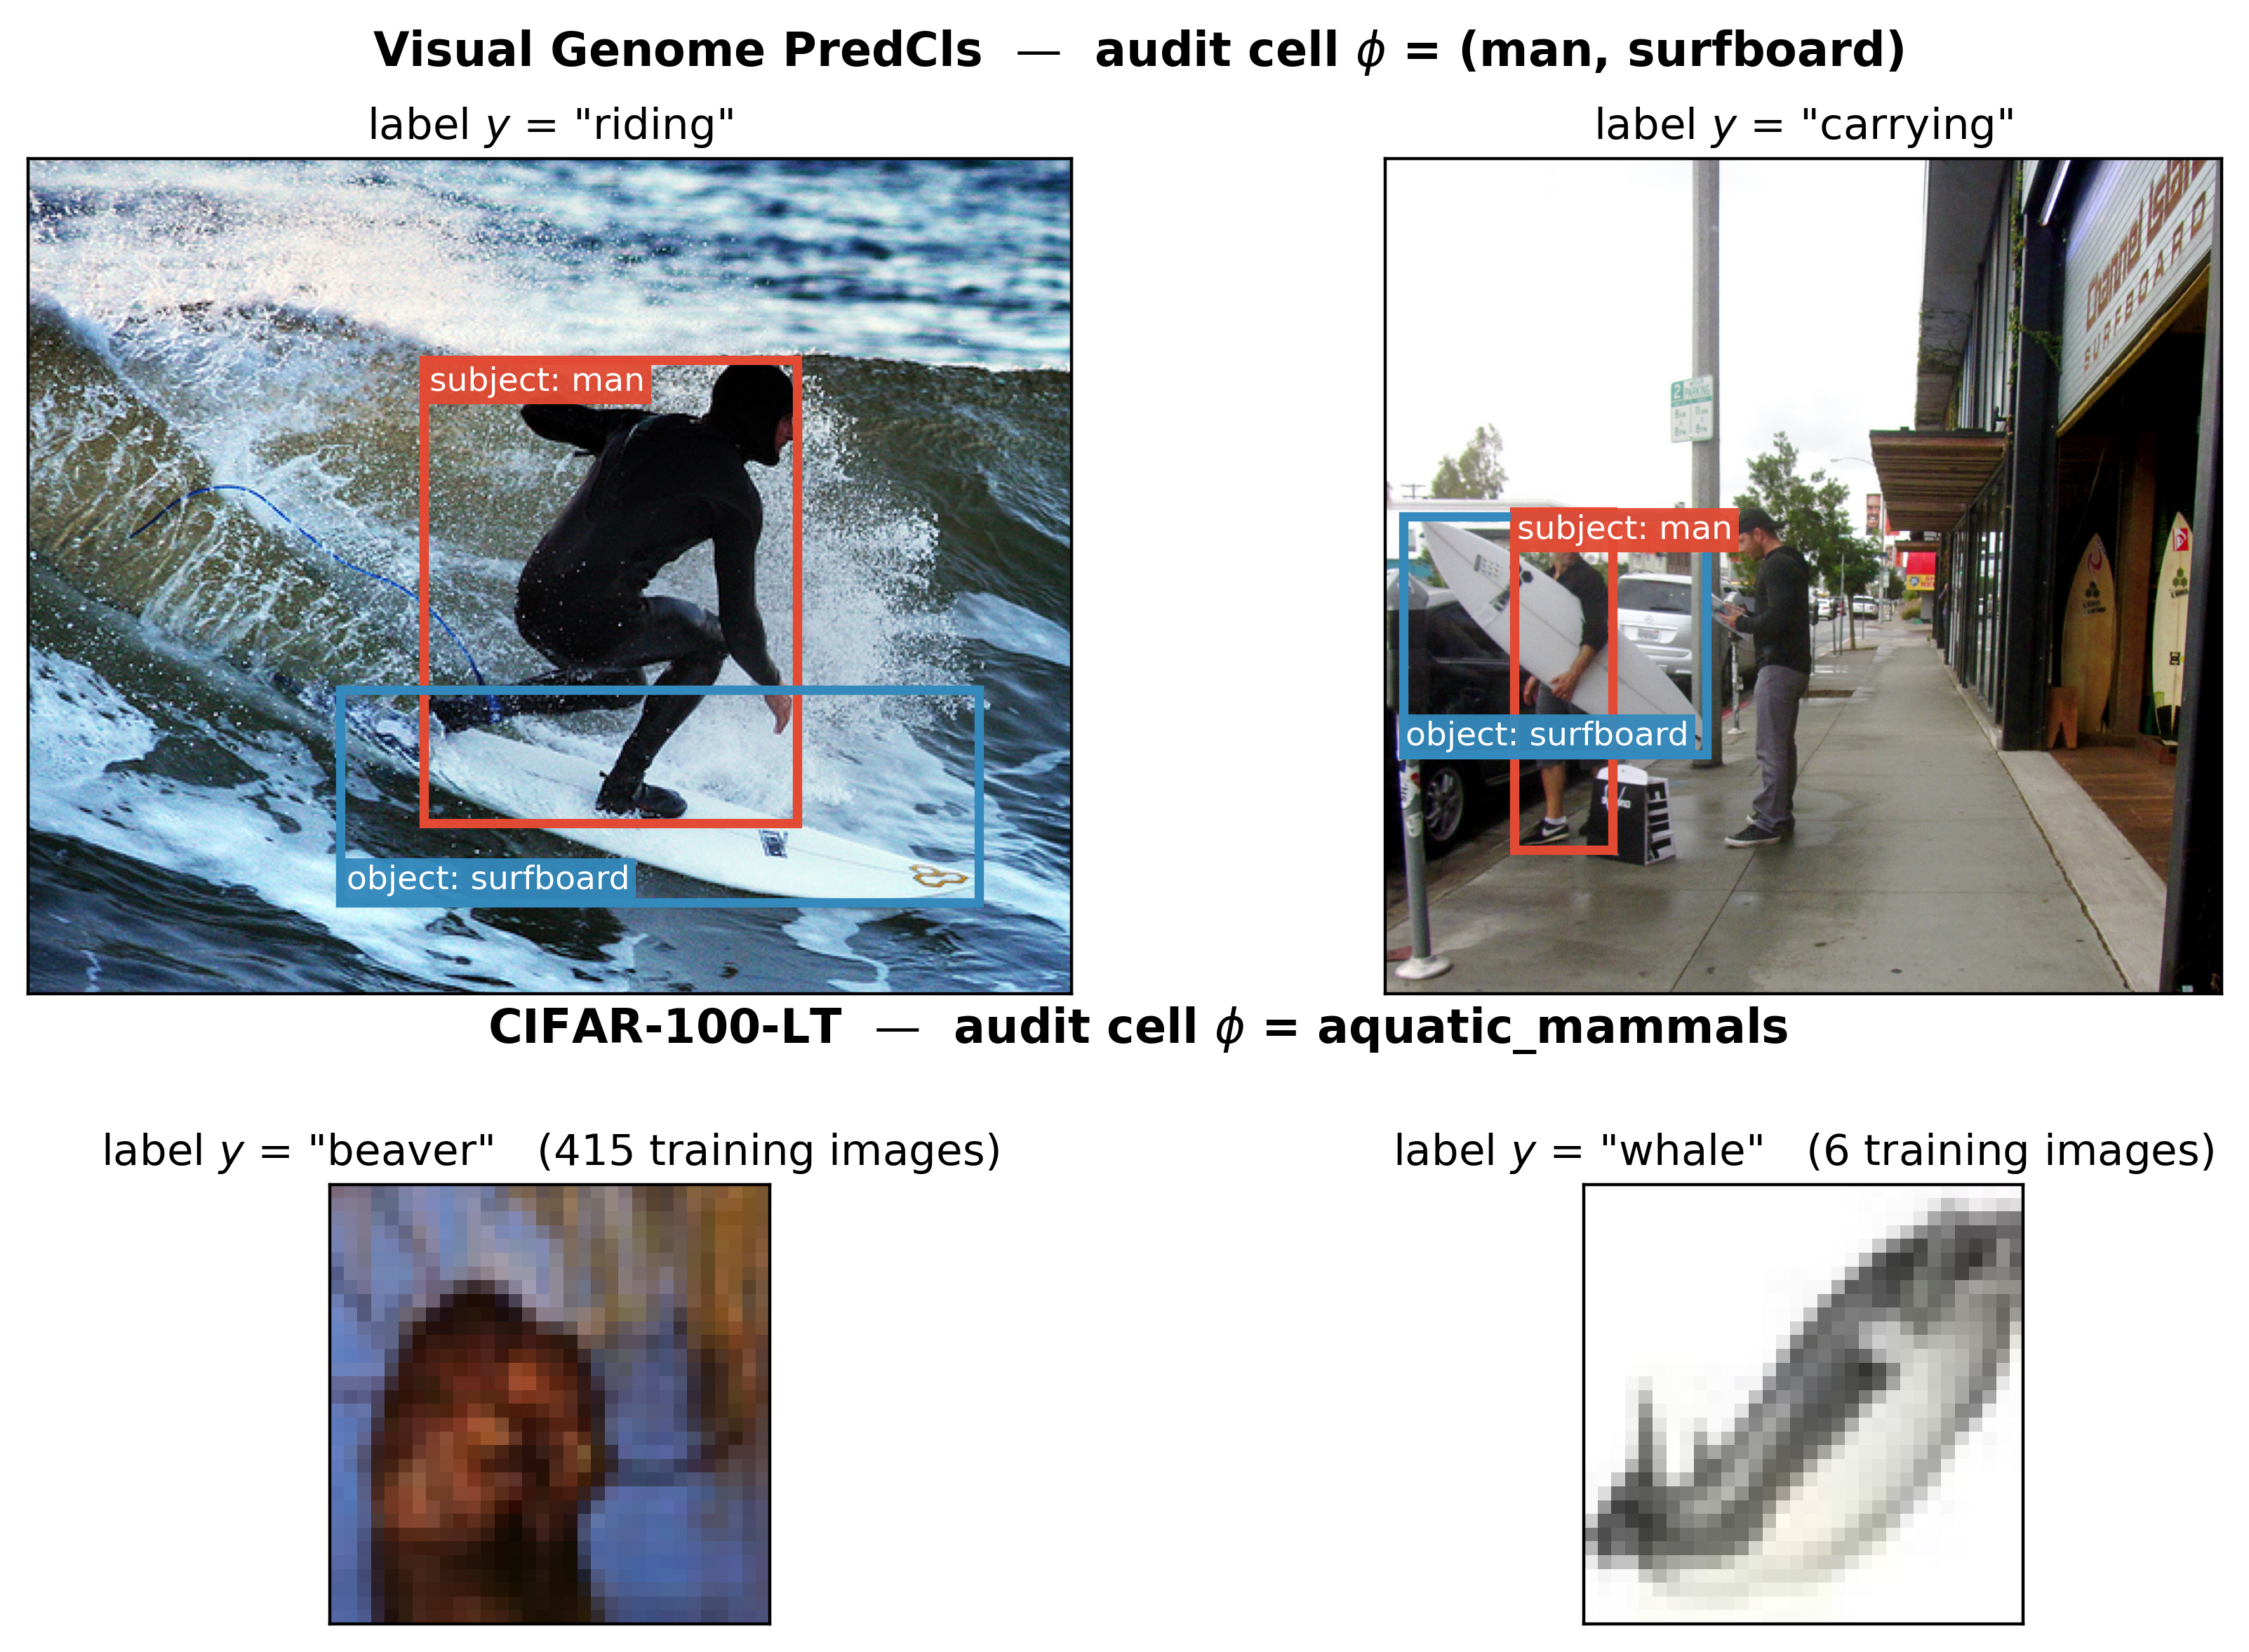
\includegraphics[width=\textwidth]{figures/fig6_dataset_samples.png}
\caption{\textbf{What a cell contains, on both benchmarks.} Each row shows two
real test examples that share the same declared grouping variable $\phi$ but carry
different labels -- precisely the configuration within-cell transport exploits.
\emph{Top:} two Visual Genome relations from the cell $\phi=(\text{man},
\text{surfboard})$. The class pair is identical and therefore cannot distinguish
``riding'' from ``carrying''; only the image content can, which is what
$\Delta R$ is designed to credit. Boxes are the annotated subject (red) and object
(blue) regions that MLP-SPATIAL turns into geometry features and MLP-VISUAL crops and
encodes with CLIP. \emph{Bottom:} two CIFAR-100 test images from the superclass
$\phi=\text{aquatic\_mammals}$, drawn from opposite ends of the long-tailed training
distribution ($415$ versus $6$ training images). Crossing the labels within a row
preserves the cell and its label histogram while destroying which prediction belongs
with which instance.}
\label{fig:samples}
\end{figure*}

\begin{table}[t]
\centering
\caption{Frozen-model top-1 accuracy on VG150 PredCls. Similar accuracies do not reveal
whether the difference is transported.}
\label{tab:accuracy}
\begin{tabular}{@{}lr@{}}
\toprule
Model & Accuracy \\
\midrule
FREQ & 0.6564 \\
FREQ+OVERLAP & 0.6545 \\
MLP-CLASS & 0.6554 \\
MLP-SPATIAL & 0.6639 \\
MLP-SPATIAL+ & 0.6674 \\
\bottomrule
\end{tabular}
\end{table}

\subsection{Gain attribution for the controlled predictors}\label{sec:results}

The central result is collected in Table~\ref{tab:wager-results} and
Figure~\ref{fig:results}. MLP-CLASS improves on FREQ by $0.03386$ of quadratic score,
yet because its gain vector is constant inside every class-pair cell, the estimator
assigns that entire improvement to prior transport and precisely nothing to instance
covariance. The zero is worth dwelling on: it follows algebraically from the construction
rather than from a learned baseline happening to pass a sanity check.

Adding box geometry changes the picture. MLP-SPATIAL gains $0.04270$ over FREQ, of which
$0.02832$ survives label transport and $0.01439$ is within-group covariance (CI
$[0.01373,0.01504]$). More revealing still is the direct comparison against MLP-CLASS,
where the total gain falls to $0.00885$ only because the transported channel deteriorates by
$0.00554$ even as the covariance gain from spatial features rises by $0.01439$. The resulting covariance share
of 1.63 records a genuinely useful instance-specific change that the aggregate score
partly conceals behind a worse prior component, and it is exactly the configuration that
a ratio confined to $[0,1]$, or thresholded at $0.5$, would misdescribe.

The remaining two comparisons bracket the interesting range. MLP-SPATIAL+ adds $0.00374$
over MLP-SPATIAL, nearly all of it covariance gain at $0.00321$ (CI $[0.00289,0.00353]$),
whereas FREQ+OVERLAP supplies the opposite caution: its overlap indicator does create a
small positive covariance gain, but the accompanying negative prior term is larger, so
the model ends up worse overall. Using image-derived information is thus never treated
as an improvement in itself; both channels are reported, signs included.

\paragraph{Reading the magnitudes.} Quadratic-score units are not ones most readers
calibrate by eye, so it is worth anchoring them in the rank-based metrics this
literature reports. Where both channels point the same way the correspondence is
straightforward: MLP-SPATIAL-S's $\widehat{\Delta R}=+0.01023$ over MLP-CLASS-S
accompanies $+0.51$ points of top-1 predicate accuracy, $+0.60$ of mean reciprocal rank
and $+0.86$ of recall@5, so in these data a hundredth of quadratic-score gain is worth
roughly half an accuracy point. The covariance channel is not, however, a re-description
of any rank metric, and the real-pixel comparison of Section~\ref{sec:vgvisual} is
where that becomes visible: there $\widehat{\Delta R}=+0.00641$ while top-1 accuracy
falls by $3.07$ points and recall@5 by $2.21$. Prior-matching both models before scoring
narrows the accuracy gap to $2.17$ points without closing it. The rank metrics aggregate
the two channels into one number; when the channels carry opposite signs, as they do
here, no single such number can represent both, which is precisely the situation the
decomposition exists to report.

\begin{table*}[t]
\centering
\caption{WAGER decomposition on 227,337 identified VG150 PredCls relations. Gains use
the quadratic score. CI is image-cluster robust; $p$ is the 499-shift relation-level
randomization diagnostic (granularity floor $.002$). ``--'' denotes an undefined share
because total gain is negative. The MLP-CLASS row's zero-width interval is exact by
construction, not a sampling statement: a gain vector constant within every cell makes
the antisymmetric kernel identically zero (Theorem~\ref{thm:population}), so no
variability exists for the interval to measure.}
\label{tab:wager-results}
\resizebox{\textwidth}{!}{%
\begin{tabular}{@{}llrrrrr@{}}
\toprule
New model & Old model & $\widehat{\Delta T}$ & $\widehat{\Delta P}$ &
$\widehat{\Delta R}$ (95\% CI) & $\widehat\rho$ & $p$ \\
\midrule
FREQ+OVERLAP & FREQ & $-0.01229$ & $-0.01430$ & $0.00202\,[0.00168,0.00235]$ & -- & .002 \\
MLP-CLASS & FREQ & $0.03386$ & $0.03386$ & $0.00000\,[0.00000,0.00000]$ & 0.00 & .724 \\
MLP-SPATIAL & FREQ & $0.04270$ & $0.02832$ & $0.01439\,[0.01373,0.01504]$ & 0.34 & .002 \\
MLP-SPATIAL+ & FREQ & $0.04644$ & $0.02885$ & $0.01760\,[0.01686,0.01834]$ & 0.38 & .002 \\
MLP-SPATIAL & MLP-CLASS & $0.00885$ & $-0.00554$ & $0.01439\,[0.01373,0.01504]$ & 1.63 & .002 \\
MLP-SPATIAL+ & MLP-SPATIAL & $0.00374$ & $0.00053$ & $0.00321\,[0.00289,0.00353]$ & 0.86 & .002 \\
\bottomrule
\end{tabular}
}
\end{table*}

\begin{figure*}[t]
\centering
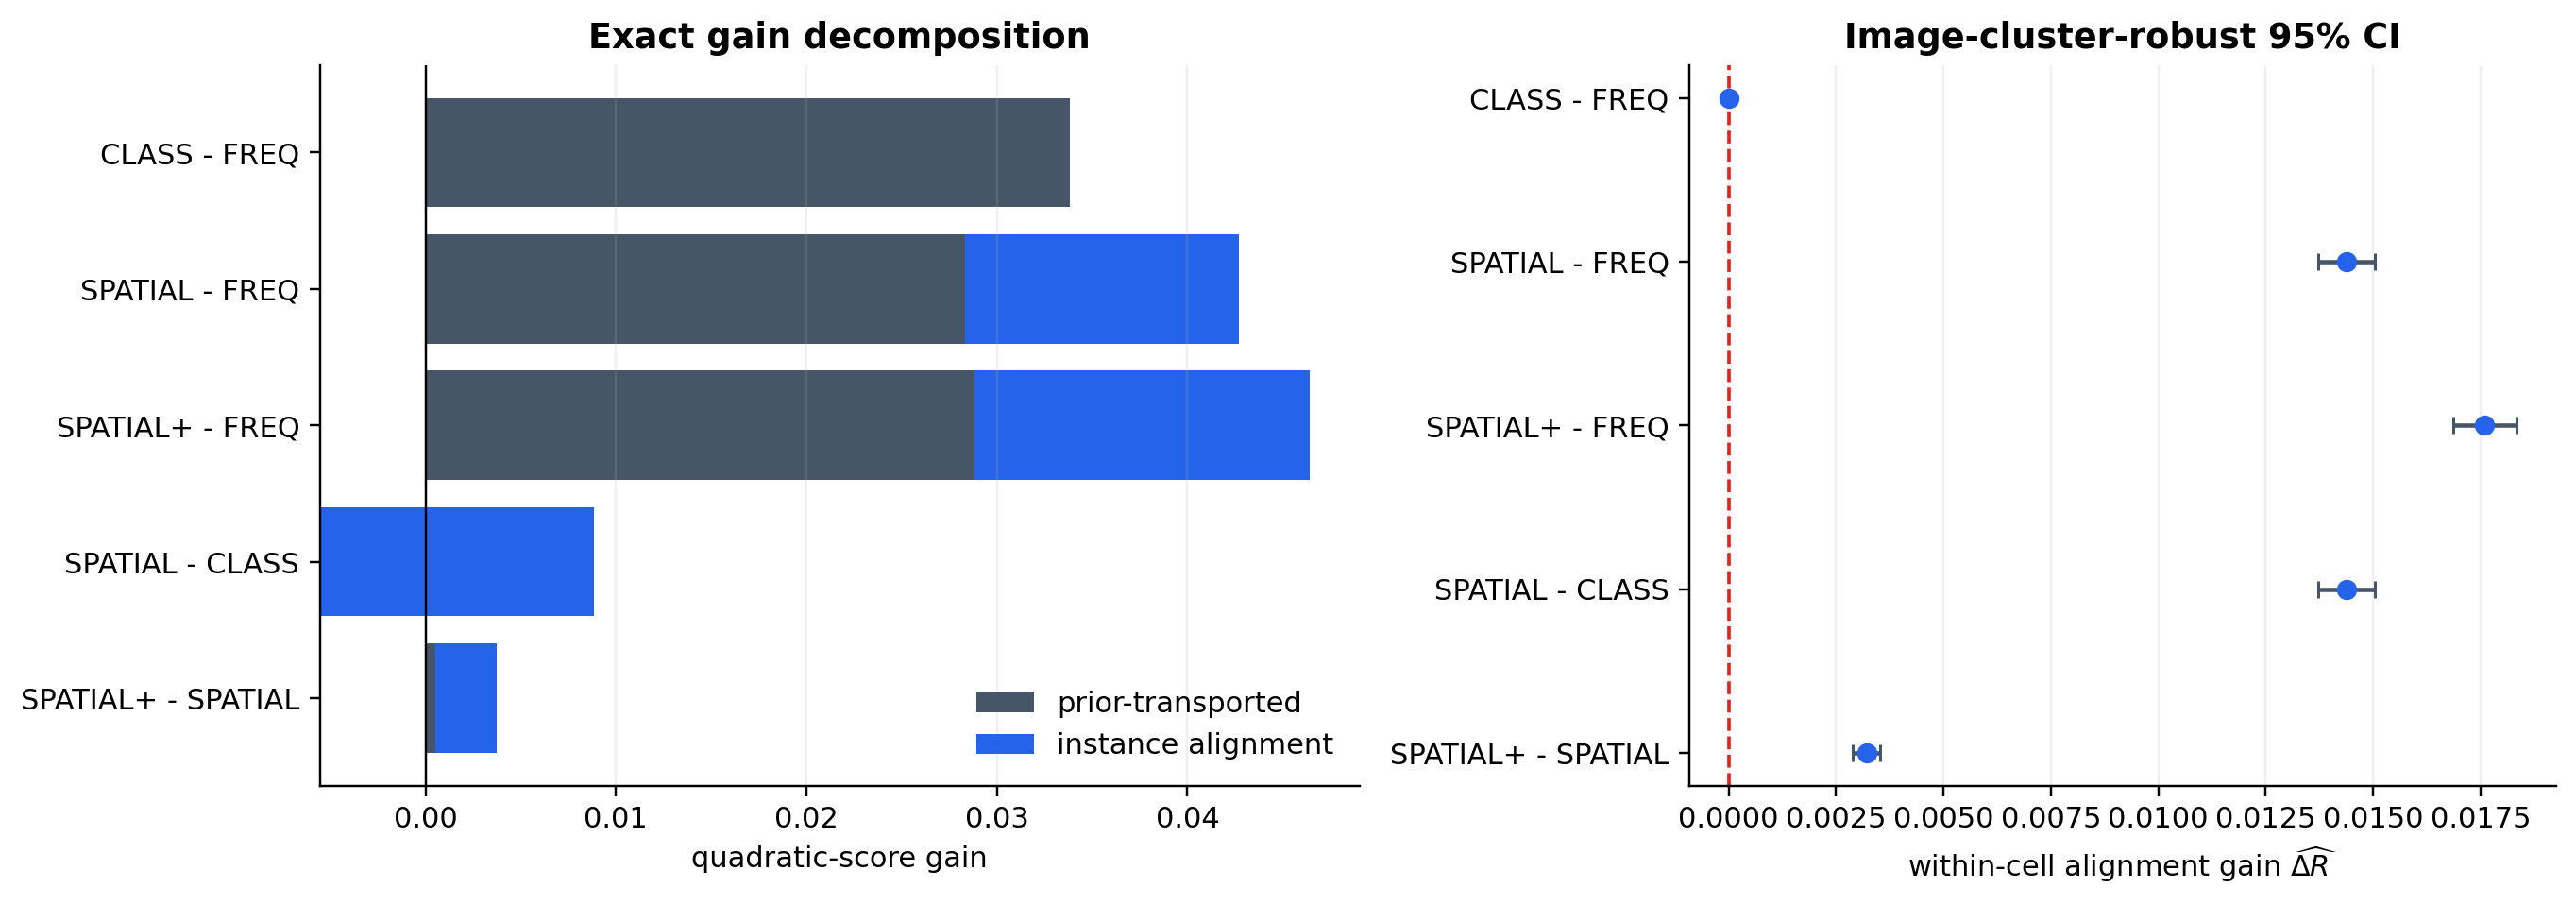
\includegraphics[width=\textwidth]{figures/fig4_new_results.png}
\caption{\textbf{Direct model-pair attribution.} Left: exact decomposition of each
positive gain into transported and within-group covariance components (the negative
prior term for SPATIAL--CLASS extends left of zero). Right: primary covariance estimates
with image-cluster-robust intervals.}
\label{fig:results}
\end{figure*}

\paragraph{Reading $\widehat{\Delta T}$ as a comparative forecast test.}
Corollary~\ref{cor:dm} identifies $\widehat{\Delta T}$ and its image-clustered interval in Table
\ref{tab:wager-results} as a grouped Diebold--Mariano statistic and interval, on the identified subsample, for
each pair's paired score differential, so every row already reports what that classical
test would report. What it does not report is the next two columns: whether MOTIFS-TDE
(Section~\ref{sec:sggaudit}) or MLP-SPATIAL beat their baseline for a reason a
frequency-only remodeling of the same benchmark could not reproduce, which is the
question $\widehat{\Delta P}$ and $\widehat{\Delta R}$ answer and DM/GW do not ask.


\subsection{Real pixels against a geometric proxy, in full}\label{app:vgvisual-full}

None of the predictors above ever sees an image: they are functions of the class pair and,
for MLP-SPATIAL(+), of box coordinates recorded in the annotation. Since box geometry is
only a proxy for image content, a sceptical reader may ask whether the covariance channel
responds to pixel evidence or merely to that proxy. Figure~\ref{fig:samples} sharpens the
question --- the cell $\phi=(\text{man},\text{surfboard})$ holds both ``riding'' and
``carrying'', and what distinguishes them is what the photograph shows.

MLP-VISUAL answers it. Subject and object regions are cropped from the original image and
each encoded by a frozen CLIP ViT-B/32 encoder \citep{radford2021learning}; the two
$512$-dimensional embeddings are concatenated with the class embeddings MLP-CLASS already
uses and passed to a small trained head. Because CLIP is never fine-tuned, whatever
covariance the model gains reflects information its pretraining already recovered from
pixels rather than representation learning on Visual Genome.

Encoding every training relation with CLIP is expensive, so MLP-VISUAL must be trained on a
subsample; setting a subsampled model against the full-data MLP-SPATIAL would confound
feature content with training-set size. All three compared predictors are therefore
retrained on one fixed, seeded subsample of $100{,}000$ of the $532{,}987$ training
relations, written MLP-CLASS-S, MLP-SPATIAL-S and MLP-VISUAL-S, so any gap between them
isolates the features. The audit still uses the full $229{,}605$-relation test split with
the same class-pair $\phi$ and image-clustered intervals.

\paragraph{Result.} By any aggregate measure the CLIP model is the worst of the three: top-1
accuracy $0.6161$ against $0.6467$ for MLP-SPATIAL-S and $0.6416$ for MLP-CLASS-S, and a
quadratic score $0.04655$ below MLP-SPATIAL-S. An evaluator reading either number would
discard it.

The decomposition contradicts that reading on the axis that matters. Against MLP-SPATIAL-S
the CLIP model loses $0.05296$ of transported gain while \emph{gaining} $0.00641$ of
covariance (95\% CI $[0.00514,0.00769]$, randomization $p=.002$): its entire deficit sits in
the transported channel and its within-cell discrimination is significantly better, not
worse. Against the class-only baseline the point is plainer still --- pixels buy $0.01665$
of covariance where box geometry buys $0.01023$, with well-separated intervals. Real image
content carries more case-specific signal than the geometric proxy standing in for it.

A plausible mechanism, stated as hypothesis rather than finding: the $1024$ CLIP dimensions
dominate the $64$ dimensions of class embedding the head also receives, so the model fits
VG150's class-pair frequency structure markedly less well than a predictor built around it. A
benchmark whose headline metric rewards transported gain will punish this model, and the
aggregate numbers duly do. What the decomposition adds is that the punishment is not for
failing to use the image. Two falsification checks, reported in
Section~\ref{app:implementation}, support that reading: correcting a model's within-cell
prior towards the training histogram registers as almost pure transported movement
($+0.02401$ against $+0.00111$ of covariance), as a correction carrying no case-level
information must, and applied to the CLIP model it halves the aggregate deficit ($-0.04655$
to $-0.02143$) while the covariance advantage persists ($+0.00752$, and $+0.00663$ when both
models are corrected) and survives confidence matching ($+0.00467$, CI
$[+0.00314,+0.00621]$).

\begin{table}[t]
\centering
\caption{Matched-subsample real-pixel study on the full VG150 test split (coverage
$99.0\%$, as in Table~\ref{tab:wager-results}). All three predictors are trained on the
same $100{,}000$ relations and differ only in features. CI is image-cluster robust on
$\widehat{\Delta R}$; $p$ is the 499-shift randomization diagnostic.}
\label{tab:vgvisual}
\resizebox{\textwidth}{!}{%
\begin{tabular}{@{}llrrrr@{}}
\toprule
New model & Old model & $\widehat{\Delta T}$ & $\widehat{\Delta P}$ &
$\widehat{\Delta R}$ (95\% CI) & $p$ \\
\midrule
MLP-SPATIAL-S & MLP-CLASS-S   & $0.00503$  & $-0.00520$ & $0.01023\,[0.00967,0.01079]$ & .002 \\
MLP-VISUAL-S  & MLP-CLASS-S   & $-0.04152$ & $-0.05816$ & $0.01665\,[0.01534,0.01796]$ & .002 \\
MLP-VISUAL-S  & MLP-SPATIAL-S & $-0.04655$ & $-0.05296$ & $0.00641\,[0.00514,0.00769]$ & .002 \\
\bottomrule
\end{tabular}
}
\end{table}

\begin{figure*}[t]
\centering
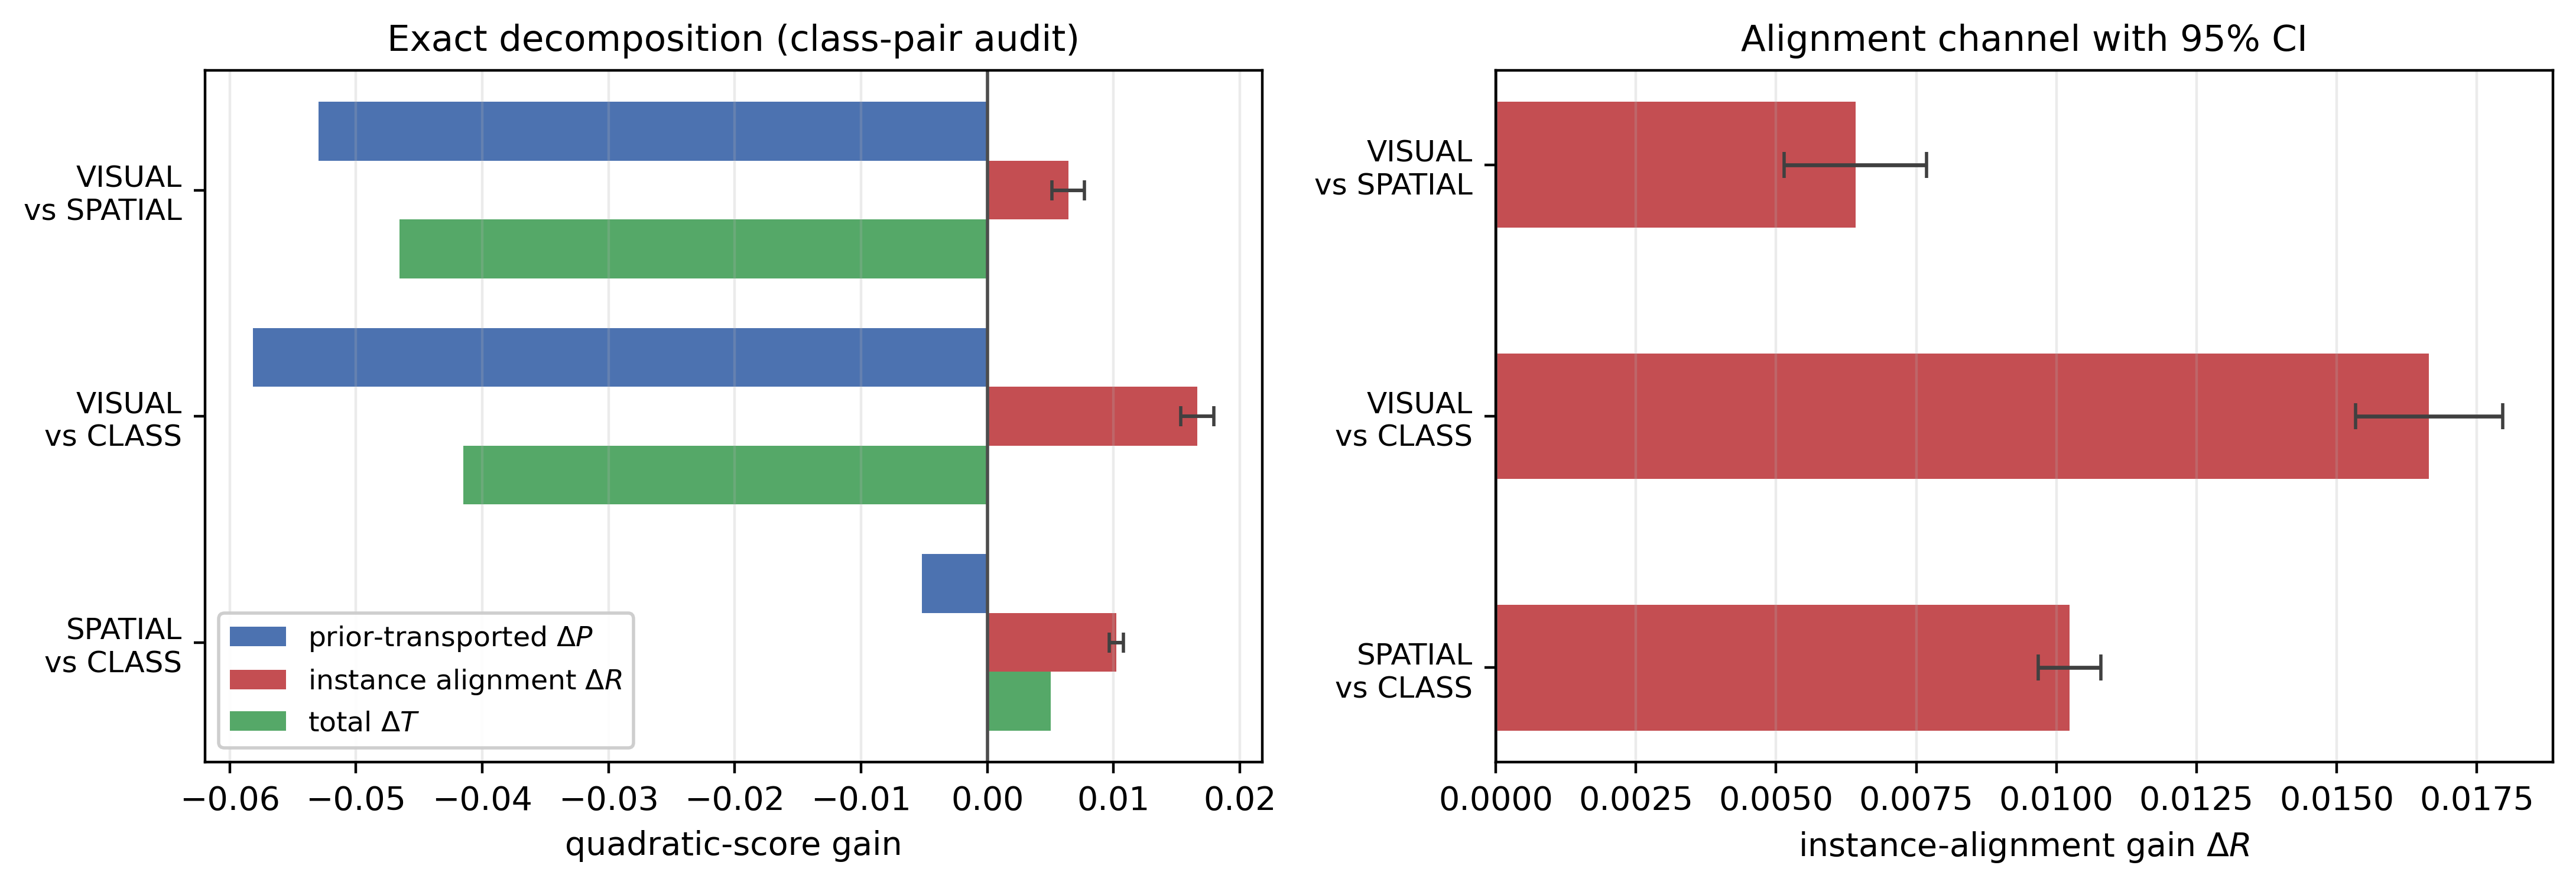
\includegraphics[width=\textwidth]{figures/fig7_vg_visual.png}
\caption{\textbf{Pixels beat geometry on covariance while losing on the aggregate.}
Left: the exact decomposition for the three matched-subsample pairs. Both comparisons
involving the CLIP model have strongly negative totals (green) driven entirely by the
transported channel (blue), while their covariance channel (red) is positive in every case.
Right: the covariance channel alone, with 95\% image-clustered intervals. Replacing box
geometry with real image content raises within-group covariance from $0.01023$ to $0.01665$
over the same class-only baseline.}
\label{fig:vgvisual}
\end{figure*}


\subsection{Sensitivity analyses}\label{sec:ablations}

For MLP-SPATIAL versus MLP-CLASS, the conclusion survives every planned sensitivity
check (Table~\ref{tab:sensitivity}). Changing from the quadratic to a probability-floored
log score changes scale ($0.01439$ to $0.06536$) but not sign or significance.
The coverage column matters for reading the rows against each other, and earlier
versions of this table omitted it. Each row targets the identified subpopulation its own
setting defines, so the minimum-cell-size rows are not four estimates of one quantity:
raising the minimum from $2$ to $20$ drops coverage from $99.0\%$ to $86.7\%$ and changes
the estimand along with the estimator. That the estimate moves so little across them
($0.01439$ to $0.01225$) is therefore mild evidence of stability rather than a
sensitivity analysis holding the target fixed.

Coarsening $\phi$ from the class pair to subject class increases the credited covariance
to $0.02181$. Proposition~\ref{prop:coarsen} identifies why: the coarser cell's estimate
equals the class-pair estimate's conditional average plus a between-class-pair covariance
term, and that term is positive here, meaning some of the credited gain reflects
class-pair-level structure that the finer audit had already correctly assigned to
$\Delta P$. This is precisely the sense in which the class-pair audit is the conservative
choice: it is not that coarsening is wrong, but that it cannot be assumed neutral, and
only the finer partition's estimate isolates covariance gain net of every prior regularity
expressible in $\phi$. The same class-pair-versus-subject-only pair also instantiates
Proposition~\ref{prop:sensitivity} directly, with the subject class playing the role of
the unrecorded confounder $Z$: Table~\ref{tab:sensitivity-numeric} in
Section~\ref{app:sensitivity} reports that the resulting bias of $0.00742$ is comfortably
inside the Cauchy--Schwarz bound, though the bound is loose enough at $K=50$ that it
would remain satisfied for a $\bar\rho$ three orders of magnitude smaller than one.
Raising the minimum cell size from 2 to 5, 10, and 20 yields
$0.01395$, $0.01330$, and $0.01225$; all cluster-robust lower limits remain positive.
The procedure itself has no smoothing strength, split fraction, or decision threshold
to tune.

\begin{table}[t]
\centering
\caption{Sensitivity of the MLP-SPATIAL vs.\ MLP-CLASS decomposition to score, audit
granularity, and minimum cell size. CI is image-cluster robust on $\widehat{\Delta R}$.}
\label{tab:sensitivity}
\small
\begin{tabular}{@{}llrr@{\,}rr@{}}
\toprule
Factor & Setting & $\widehat{\Delta T}$ & \multicolumn{1}{r}{$\widehat{\Delta R}$ (95\% CI)} & Cells &
Cov. \\
\midrule
Score & Brier (def.) & $0.00885$ & $0.01439\,[0.01373,0.01504]$ & 6346 & $99.0\%$ \\
Score & Log (floored) & $0.04297$ & $0.06536\,[0.06294,0.06779]$ & 6346 & $99.0\%$ \\
Cell $\phi$ & class pair (def.) & $0.00885$ & $0.01439\,[0.01373,0.01504]$ & 6346 & $99.0\%$ \\
Cell $\phi$ & subject only & $0.00943$ & $0.02181\,[0.02079,0.02283]$ & 150 & $100.0\%$ \\
Min.\ cell size & 2 (def.) & $0.00885$ & $0.01439\,[0.01373,0.01504]$ & 6346 & $99.0\%$ \\
Min.\ cell size & 5 & $0.00772$ & $0.01395\,[0.01329,0.01462]$ & 4060 & $96.3\%$ \\
Min.\ cell size & 10 & $0.00683$ & $0.01330\,[0.01262,0.01398]$ & 2744 & $92.6\%$ \\
Min.\ cell size & 20 & $0.00570$ & $0.01225\,[0.01155,0.01295]$ & 1757 & $86.7\%$ \\
\bottomrule
\end{tabular}
\end{table}


\subsection{Long-tailed image classification}\label{app:lt}\label{sec:cifarlt}

Sections~\ref{sec:data}--\ref{sec:vgvisual} are all instances of one task (predicate
classification on an ordered object pair). Section~\ref{sec:related-applied} argued
that long-tailed image classification poses a structurally identical question: a
class-frequency prior can be fit better without any per-instance improvement. We test
this directly on CIFAR-100-LT \citep{cui2019classbalanced}, an exponential-imbalance
(ratio $100$) subsample of CIFAR-100's training split with the original, balanced test
split retained for evaluation. We train ResNet-32 \citep{he2016deep} classifiers that
differ only in their per-class loss weighting: a vanilla cross-entropy baseline (CE);
class-balanced effective-number re-weighting applied from initialization (CB)
\citep{cui2019classbalanced}; and the same re-weighting deferred to the final twenty
epochs (DRW) \citep{cao2019learning}. Optimizer, schedule, augmentation, epoch budget,
and seed are identical across runs (Section~\ref{app:implementation}).

\paragraph{Choosing $\phi$.} A declared grouping variable has to predict the label without
determining it, and this second benchmark makes the constraint unusually easy to
violate. Were $\phi$ taken to be the fine class label itself, every cell would be
label-homogeneous, within-cell transport would have nothing to cross, and
$\widehat{\Delta R}$ would come out identically zero -- an algebraic artifact wearing the
appearance of a finding. CIFAR-100's own 20 coarse superclasses avoid this, each
gathering five fine labels into a cell of $500$ balanced test images, which is
structurally the situation of a VG class-pair cell holding several predicates
(Figure~\ref{fig:samples}). Alongside the superclass audit we report two further
declared priors: the trivial coarsening to a single global cell, which audits against
the global class marginal and so instantiates Proposition~\ref{prop:coarsen} in a second
domain, and a partition into head, medium and tail training-frequency tiers. CIFAR-100
test images are independent, unlike the several relations VG draws from one photograph,
so no cluster grouping is required and the plain H\'ajek interval of
Section~\ref{sec:inference} applies directly. One semantic point matters in this domain:
transport uses each cell's \emph{test} label histogram, which on CIFAR-100-LT is
balanced. A positive $\Delta P$ here therefore records movement \emph{toward} the
balanced test marginal -- undoing the training-frequency skew -- which is precisely the
adjustment long-tailed evaluation is designed to reward; a transported gain is a
description of where score was earned, not an accusation
(Section~\ref{sec:discussion}).

\paragraph{Result.} The three classifiers reach top-1 accuracies of $0.3662$ (CE),
$0.2627$ (CB) and $0.3874$ (DRW), so re-weighting from initialization degrades the
classifier substantially while the deferred schedule delivers the improvement it was
designed to produce. Table~\ref{tab:cifar} decomposes both gains against the superclass
audit.

Of the two, the class-balanced run is the more instructive, precisely because its
aggregate score conceals almost everything of interest. On the quadratic score it gains
$+0.00143$ over the baseline, a difference small enough that a reader working from the
headline number alone would reasonably conclude that re-weighting had changed very
little. The decomposition tells another story: within superclasses the
transported channel improves by $+0.19713$ while within-group covariance deteriorates
by $-0.19569$ (95\% CI $[-0.20728,-0.18411]$), so the near-zero total is not a small
effect but two large ones that happen to cancel.

\paragraph{A calibration-matched regime.} A channel split of that shape could, however,
be produced by confidence scaling alone. Under the quadratic score the covariance channel
is a covariance between probability movements and labels
(Eq.~\eqref{eq:cov-id}), and a monotone recalibration moves it: softening an
overconfident model transfers score mass from the covariance channel to the transported channel while
adding no information about any individual image. The baseline invites exactly this
concern, assigning a mean maximum probability of $0.764$ while being correct on only
$0.3662$ of the test set. We therefore repeat the audit in a calibration-matched regime:
each model's temperature is chosen by held-out likelihood on a calibration half of the
test split ($T^*=2.85$ for CE, $3.51$ for CB, $2.61$ for DRW), the decomposition is
computed on the disjoint audit half, and the whole procedure is repeated over twenty
random splits (Table~\ref{tab:cifar-cal}). The regime's necessity is quantified by its
control row: recalibrating the baseline alone -- a transformation carrying no instance
information -- moves the channels by $+0.380$ (prior) and $-0.175$ (covariance), so the
raw split does mix calibration with discrimination.

The calibration-matched rows then separate the two schedules cleanly, and more sharply
than the raw ones. CB's covariance deficit does not shrink but widens, to
$-0.23991\,(0.00491)$: the model re-weighted from initialization has genuinely lost
within-superclass discrimination -- a real degradation that the ten-point accuracy drop
records independently -- and its near-zero raw total reflects that loss offset by its
softer, better-calibrated confidence. DRW inverts the reading its raw split suggests.
Raw, its $+0.06712$ gain divides roughly two-thirds transported to one-third covariance gain;
calibration-matched, the improvement is $+0.02173\,(0.00275)$ of which
$+0.01957\,(0.00329)$ is within-group covariance while the transported channel is close to zero
($+0.00216\,(0.00410)$). What survives calibration matching is precisely the component
the deferred schedule was designed to buy -- per-instance discrimination, concentrated
on rare classes (Table~\ref{tab:cifar-tier}) -- while the apparently transported
share of its raw gain was largely the calibration difference between the two runs.
Neither an accuracy difference nor an aggregate score exposes either composition, which
is the practical argument for reporting the two channels, in both regimes, instead of
their sum.

\begin{table}[t]
\centering
\caption{Raw and calibration-matched decompositions on CIFAR-100-LT at the superclass
audit. Temperatures are fitted by likelihood on a held-out calibration half of the test
split; every decomposition uses the disjoint audit half; entries are means (sd) over
twenty random splits. The final row is the control: recalibrating the baseline alone
carries no instance information yet moves both channels substantially.}
\label{tab:cifar-cal}
\resizebox{\textwidth}{!}{%
\begin{tabular}{@{}llrrr@{}}
\toprule
Comparison & Regime & $\widehat{\Delta T}$ & $\widehat{\Delta P}$ &
$\widehat{\Delta R}$ \\
\midrule
CB vs CE  & raw                 & $+0.00208\,(0.00642)$ & $+0.19635\,(0.00369)$ & $-0.19427\,(0.00632)$ \\
CB vs CE  & calibration-matched & $-0.12912\,(0.00373)$ & $+0.11079\,(0.00372)$ & $-0.23991\,(0.00491)$ \\
DRW vs CE & raw                 & $+0.06712\,(0.00865)$ & $+0.04258\,(0.00463)$ & $+0.02454\,(0.00685)$ \\
DRW vs CE & calibration-matched & $+0.02173\,(0.00275)$ & $+0.00216\,(0.00410)$ & $+0.01957\,(0.00329)$ \\
\midrule
CE recalibrated vs CE & control & $+0.20495\,(0.00420)$ & $+0.37960\,(0.00268)$ & $-0.17464\,(0.00455)$ \\
\bottomrule
\end{tabular}
}
\end{table}

\paragraph{Seeds, imbalance ratios, and a post-hoc arm.} A decomposition computed from
one trained pair carries only test-set sampling uncertainty, which is not the uncertainty
relevant to a claim about a training \emph{method}. We therefore retrained the triple at
two further seeds at the primary ratio and at imbalance ratios $10$ and $50$, and added a
fourth arm: post-hoc logit adjustment (LA), which divides the baseline's predictions by
the training class prior without retraining \citep{menon2021long}. Every configuration is
audited in both regimes; Table~\ref{tab:cifar-robust} reports the calibration-matched
covariance channel, which is the one the preceding paragraphs interpret.

Three things follow. First, the class-balanced run's covariance loss is not a
misconfiguration but a systematic function of imbalance severity: $-0.069$ at ratio $10$,
$-0.244$ at $50$, and $-0.251\,(0.011)$ across three seeds at $100$, tracking an accuracy
penalty that grows from $2.3$ to $10.4$ points over the same range. Second, the deferred
schedule's covariance gain is positive at every ratio and in every seed, but its magnitude
varies roughly fourfold across seeds at ratio $100$ ($+0.007$ to $+0.031$). We therefore
report the spread rather than a seed-level interval: the direction replicates, the
magnitude is seed-sensitive, and the gap between the tight within-run intervals of
Table~\ref{tab:cifar} and this across-seed spread is exactly why a method-level claim
needs replication rather than a single audit.

Third, LA is an instructive falsification of a natural expectation. A purely post-hoc
prior correction might be expected to register as almost pure transported channel, as the
within-cell prior matching of Section~\ref{sec:vgvisual} does. It does not:
calibration-matched, LA reads as almost entirely covariance gain ($+0.022$ to $+0.038$) with a
transported channel near zero, while achieving the best balanced accuracy of any arm at every
ratio. The reason is visible in the construction. Dividing by the \emph{global} class
prior is not a within-superclass histogram move, because fine classes inside a superclass
differ in training frequency, and the correction it applies is multiplicative in each
example's own predicted probabilities --- it changes rankings where the model already
carried latent evidence. The two post-hoc corrections in this paper therefore land in
opposite channels, and correctly so: transport separates adjustments that act on the
cell's label histogram from adjustments that act on individual predictions.

\begin{table}[t]
\centering
\caption{Calibration-matched covariance gain across seeds and imbalance ratios, with
balanced test accuracy for each arm. LA is post-hoc logit adjustment applied to the
baseline. The class-balanced deficit scales with imbalance severity; the deferred
schedule's gain is positive throughout but seed-sensitive in magnitude; the post-hoc
correction lands in the covariance channel rather than the transported channel.}
\label{tab:cifar-robust}
\resizebox{\textwidth}{!}{%
\begin{tabular}{@{}llrrrrrrr@{}}
\toprule
& & \multicolumn{4}{c}{Top-1 accuracy} & \multicolumn{3}{c}{$\widehat{\Delta R}$ vs.\ CE (calibration-matched)} \\
\cmidrule(lr){3-6}\cmidrule(l){7-9}
Ratio & Seed & CE & CB & DRW & LA & CB & DRW & LA \\
\midrule
$10$  & 0 & $0.5388$ & $0.5154$ & $0.5447$ & $0.5497$ & $-0.06903$ & $+0.00617$ & $+0.02222$ \\
$50$  & 0 & $0.4256$ & $0.3242$ & $0.4399$ & $0.4550$ & $-0.24409$ & $+0.01903$ & $+0.03768$ \\
$100$ & 0 & $0.3662$ & $0.2627$ & $0.3874$ & $0.3959$ & $-0.23936$ & $+0.01987$ & $+0.03449$ \\
$100$ & 1 & $0.3614$ & $0.2287$ & $0.3762$ & $0.3877$ & $-0.26176$ & $+0.00748$ & $+0.02672$ \\
$100$ & 2 & $0.3687$ & $0.2481$ & $0.3968$ & $0.4024$ & $-0.25213$ & $+0.03124$ & $+0.03601$ \\
\midrule
\multicolumn{2}{@{}l}{$100$, mean (sd)} & & & & &
$-0.25108\,(0.01124)$ & $+0.01953\,(0.01188)$ & $+0.03241\,(0.00498)$ \\
\bottomrule
\end{tabular}
}
\end{table}

Where the covariance gain sits is visible in Table~\ref{tab:cifar-tier} and
Figure~\ref{fig:cifar} (raw regime, primary seed). For DRW it falls where the long-tail literature intends it to,
reaching $+0.09009$ on few-shot classes and $+0.06760$ on medium-shot ones, while
many-shot classes lose $-0.07624$ as the schedule shifts capacity away from the head.
The class-balanced run reproduces that same ordering with every level displaced
downward, its many-shot covariance collapsing to $-0.41977$. What the decomposition
supplies, then, is not only how much of a long-tail gain is real but where in the
frequency spectrum it was earned.

These numbers also provide an implementation check on real inputs. Computing the
within-group covariance gain directly from the identity of Eq.~\eqref{eq:cov-id}, through a
code path that shares nothing with the transport estimator, gives $-0.19530$; multiplying
by the factor $n_c/(n_c-1)$ that Proposition~\ref{prop:attenuate} predicts, at the
$n_c=500$ of a balanced superclass cell, returns $-0.195693$ against the estimator's
$-0.19569$. The identities of Theorem~\ref{thm:population} and
Proposition~\ref{prop:attenuate} are algebraic, so this verifies the implementation
rather than the theory; the point of the check is that two independent code paths agree
to the fifth decimal on real trained models, not only on the synthetic populations used
in the unit tests.

\begin{table}[t]
\centering
\caption{WAGER decomposition on the 10,000-image balanced CIFAR-100-LT test split.
Gains use the quadratic score; CI is the H\'ajek interval on $\widehat{\Delta R}$;
$p$ is the 499-shift randomization diagnostic, one-sided for a positive covariance gain, so the
value of $1.000$ on the CB rows records a covariance gain at the extreme negative end of
its randomization distribution.}
\label{tab:cifar}
\resizebox{\textwidth}{!}{%
\begin{tabular}{@{}llrrrr@{}}
\toprule
Comparison & Audit cell $\phi$ & $\widehat{\Delta T}$ & $\widehat{\Delta P}$ &
$\widehat{\Delta R}$ (95\% CI) & $p$ \\
\midrule
CB vs CE  & superclass (20) & $0.00143$ & $0.19713$ & $-0.19569\,[-0.20728,-0.18411]$ & $1.000$ \\
CB vs CE  & global (1)      & $0.00143$ & $0.25573$ & $-0.25430\,[-0.26801,-0.24058]$ & $1.000$ \\
CB vs CE  & tier (3)        & $0.00143$ & $0.25247$ & $-0.25103\,[-0.26453,-0.23754]$ & $1.000$ \\
\midrule
DRW vs CE & superclass (20) & $0.06606$ & $0.04206$ & $0.02400\,[0.01340,0.03460]$ & $.002$ \\
DRW vs CE & global (1)      & $0.06606$ & $0.03522$ & $0.03085\,[0.01860,0.04309]$ & $.002$ \\
DRW vs CE & tier (3)        & $0.06606$ & $0.03702$ & $0.02904\,[0.01702,0.04107]$ & $.002$ \\
\bottomrule
\end{tabular}
}
\end{table}

\begin{table}[t]
\centering
\caption{Covariance gain by training-frequency tier at the primary superclass audit.
The deferred schedule concentrates its genuine per-instance improvement on rare
classes; both methods lose covariance on the head.}
\label{tab:cifar-tier}
\begin{tabular}{@{}lrrrr@{}}
\toprule
& & \multicolumn{1}{c}{CB vs CE} & \multicolumn{2}{c}{DRW vs CE} \\
\cmidrule(l){3-3}\cmidrule(l){4-5}
Tier & $n$ & $\widehat{\Delta R}$ & $\widehat{\Delta T}$ & $\widehat{\Delta R}$ \\
\midrule
Few-shot ($<20$)        & 3000 & $-0.03337$ & $0.13785$ & $0.09009$ \\
Medium-shot ($20$--$100$) & 3500 & $-0.11075$ & $0.10799$ & $0.06760$ \\
Many-shot ($>100$)      & 3500 & $-0.41977$ & $-0.03740$ & $-0.07624$ \\
\bottomrule
\end{tabular}
\end{table}

\begin{figure*}[t]
\centering
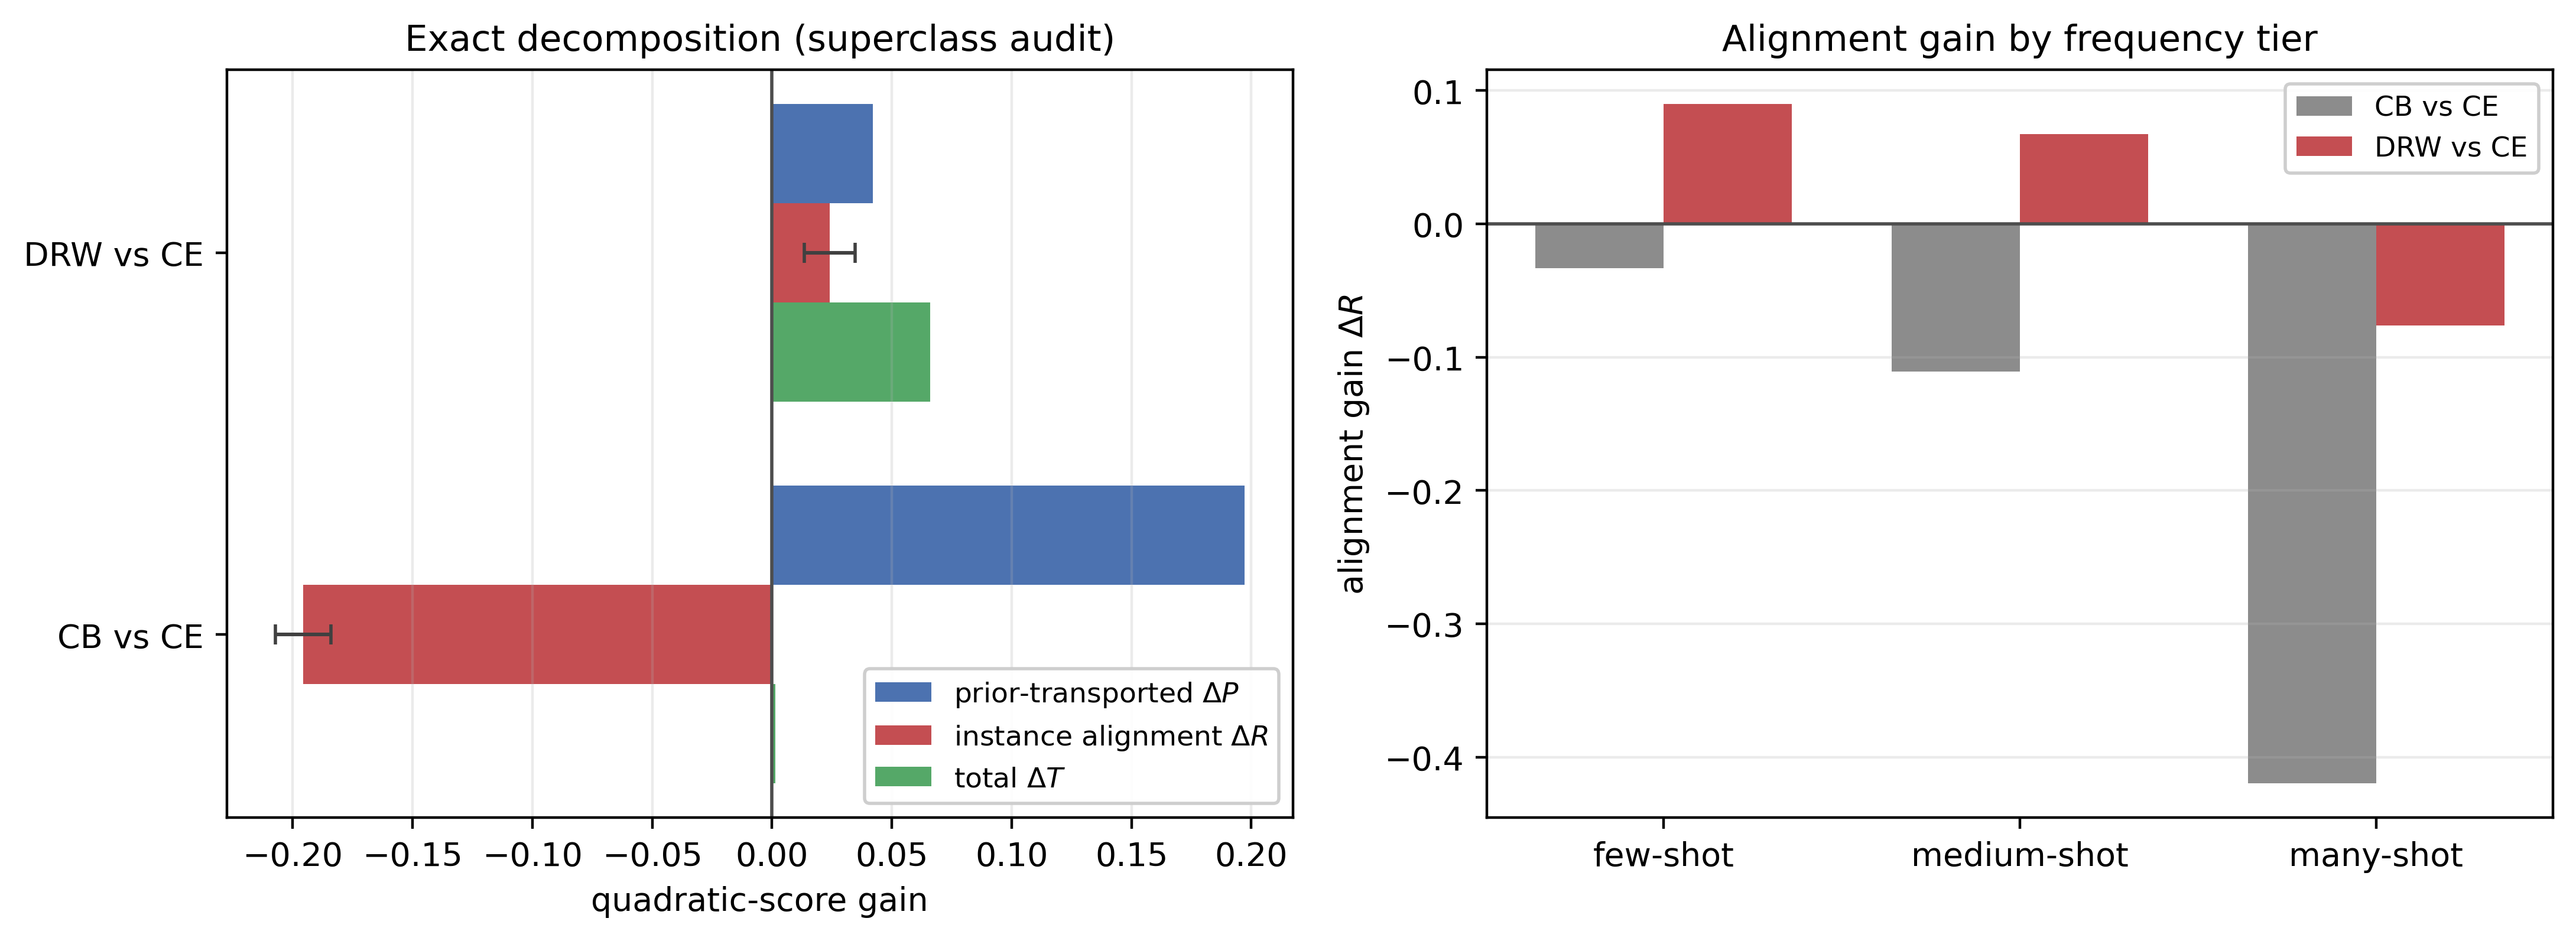
\includegraphics[width=\textwidth]{figures/fig5_cifar_lt.png}
\caption{\textbf{The same attribution transfers to a second task.} Left: exact
decomposition at the superclass audit. The CB total gain (green) is visually almost
absent at $+0.00143$ while its two channels reach $\pm0.2$ -- a near-zero aggregate
score concealing two large opposing effects. DRW's smaller total is genuinely split
between both channels. Error bars are 95\% H\'ajek intervals on $\widehat{\Delta R}$.
Right: the covariance channel by training-frequency tier, showing that DRW's genuine
per-instance gain is concentrated on rare classes and negative on the head.}
\label{fig:cifar}
\end{figure*}

Coarsening behaves as Proposition~\ref{prop:coarsen} predicts. Moving from the 20
superclass cells to a single global cell changes the credited covariance from $-0.19569$
to $-0.25430$; the difference is the between-cell covariance term, which is negative
here, so the coarse audit overstates the covariance loss by attributing to it structure
that the superclass partition correctly assigns to $\Delta P$. The finer partition is
again the conservative reading, for the same reason as in Section~\ref{sec:ablations}
and now in a second domain.

\subsection{Long-tailed text classification}\label{sec:textlt}

Sections~\ref{sec:results}--\ref{app:lt} test two vision tasks that share cached
probability vectors and grouping variables grounded in class frequency or object geometry.
To test the breadth Section~\ref{sec:discussion} claims -- any benchmark supplying two
models' full probability vectors, labels, and a declared discrete grouping variable -- we
apply the identical estimator, unmodified, to document category prediction on 20
Newsgroups \citep{lang1995newsweeder}. Neither the predictors nor the grouping variable are
visual here: documents replace images, and the declared $\phi$ is a topical grouping
rather than a spatial or class-frequency one, so a favorable result cannot be attributed
to anything specific to vision data.

We build a long-tailed training subset with the same exponential profile as
CIFAR-100-LT (imbalance ratio $100$, Section~\ref{app:lt}), applied to 20
Newsgroups' 20 fine categories, keeping the standard balanced test split ($7{,}532$
documents) untouched (Section~\ref{app:implementation}). The 20 categories fall into
six conventional coarse topics -- computing, recreation, science, politics, religion,
and classifieds -- which we use as the primary declared $\phi$, the direct analogue of
CIFAR's coarse superclasses; a global (trivial) and a training-frequency-tier partition
are reported alongside, as in Section~\ref{app:lt}. Documents are represented by a
TF-IDF vector reduced to $300$ dimensions by truncated SVD, and the three compared
classifiers -- CE, CB, and DRW -- follow the same three-arm protocol as
Section~\ref{app:lt}: an identical small MLP architecture and optimizer across runs,
differing only in per-example loss weight (Section~\ref{app:implementation}). Test
documents are independent units, so the plain H\'ajek interval of Section~\ref{sec:inference}
applies directly, as for CIFAR.

\paragraph{Result.} Table~\ref{tab:textlt} decomposes both re-weighting schedules' gain
over the cross-entropy baseline (top-1 accuracies $0.3532$ CE, $0.3960$ CB, $0.3776$
DRW). The two schedules land in opposite channels here, which is itself the finding
worth reporting: on this task it is class-balanced re-weighting from initialization, not
the deferred schedule, that buys genuine within-topic covariance gain ($+0.04317$, CI
$[0.03664,0.04970]$, $37.9\%$ of its total gain), while DRW's comparably sized total gain
($0.11490$ vs.\ CB's $0.11388$) is $98.6\%$ transported, its residual covariance
statistically indistinguishable from zero at the superclass audit ($+0.00155$, CI
$[-0.00296,0.00605]$, $p=.236$) and significantly negative once the coarser tier
partition is used instead ($-0.00901$, CI $[-0.01428,-0.00374]$). This is the reverse of
Section~\ref{app:lt}'s image-classification finding, where CB's near-zero total
masked a large covariance-gain \emph{loss} and DRW's gain was genuinely covariance-driven.
Nothing about the estimator or the construction of $\phi$ changed between the two
applications; what changed is which training recipe, on which data, buys real
per-instance discrimination -- exactly the composition question an aggregate score or an
accuracy difference alone cannot answer, now demonstrated on a domain with neither a
class-frequency table nor a spatial prior.

Coarsening moves both comparisons in the direction Proposition~\ref{prop:coarsen} allows
without requiring: CB's credited covariance falls from $0.04317$ at the superclass
partition to $0.04185$ at the global cell and $0.03578$ at the tier partition, while
DRW's changes sign twice, from a small positive residual (superclass) to a small
negative one (global) to a significant negative one (tier). None of these differences
overturns CB's conclusion, but DRW's illustrates exactly why the finest defensible
partition is the conservative default (Section~\ref{sec:coarsening}): a reader stopping
at the coarser tier partition would report a significant covariance \emph{loss} for a
method whose finer-grained residual is not distinguishable from zero.

\begin{table}[t]
\centering
\caption{WAGER decomposition on the 7,532-document balanced 20-Newsgroups-LT test
split. Gains use the quadratic score; CI is the (unclustered) H\'ajek interval on
$\widehat{\Delta R}$, documents being independent units; $p$ is the 499-shift
randomization diagnostic, one-sided for a positive covariance gain.}
\label{tab:textlt}
\resizebox{\textwidth}{!}{%
\begin{tabular}{@{}llrrrr@{}}
\toprule
Comparison & Audit cell $\phi$ & $\widehat{\Delta T}$ & $\widehat{\Delta P}$ &
$\widehat{\Delta R}$ (95\% CI) & $p$ \\
\midrule
CB vs CE  & superclass (6) & $0.11388$ & $0.07071$ & $0.04317\,[0.03664,0.04970]$ & $.002$ \\
CB vs CE  & global (1)     & $0.11388$ & $0.07203$ & $0.04185\,[0.03381,0.04990]$ & $.002$ \\
CB vs CE  & tier (3)       & $0.11388$ & $0.07810$ & $0.03578\,[0.02825,0.04331]$ & $.002$ \\
\midrule
DRW vs CE & superclass (6) & $0.11490$ & $0.11335$ & $0.00155\,[-0.00296,0.00605]$ & $.236$ \\
DRW vs CE & global (1)     & $0.11490$ & $0.11809$ & $-0.00319\,[-0.00884,0.00245]$ & $.980$ \\
DRW vs CE & tier (3)       & $0.11490$ & $0.12391$ & $-0.00901\,[-0.01428,-0.00374]$ & $1.000$ \\
\bottomrule
\end{tabular}
}
\end{table}

\begin{figure*}[t]
\centering
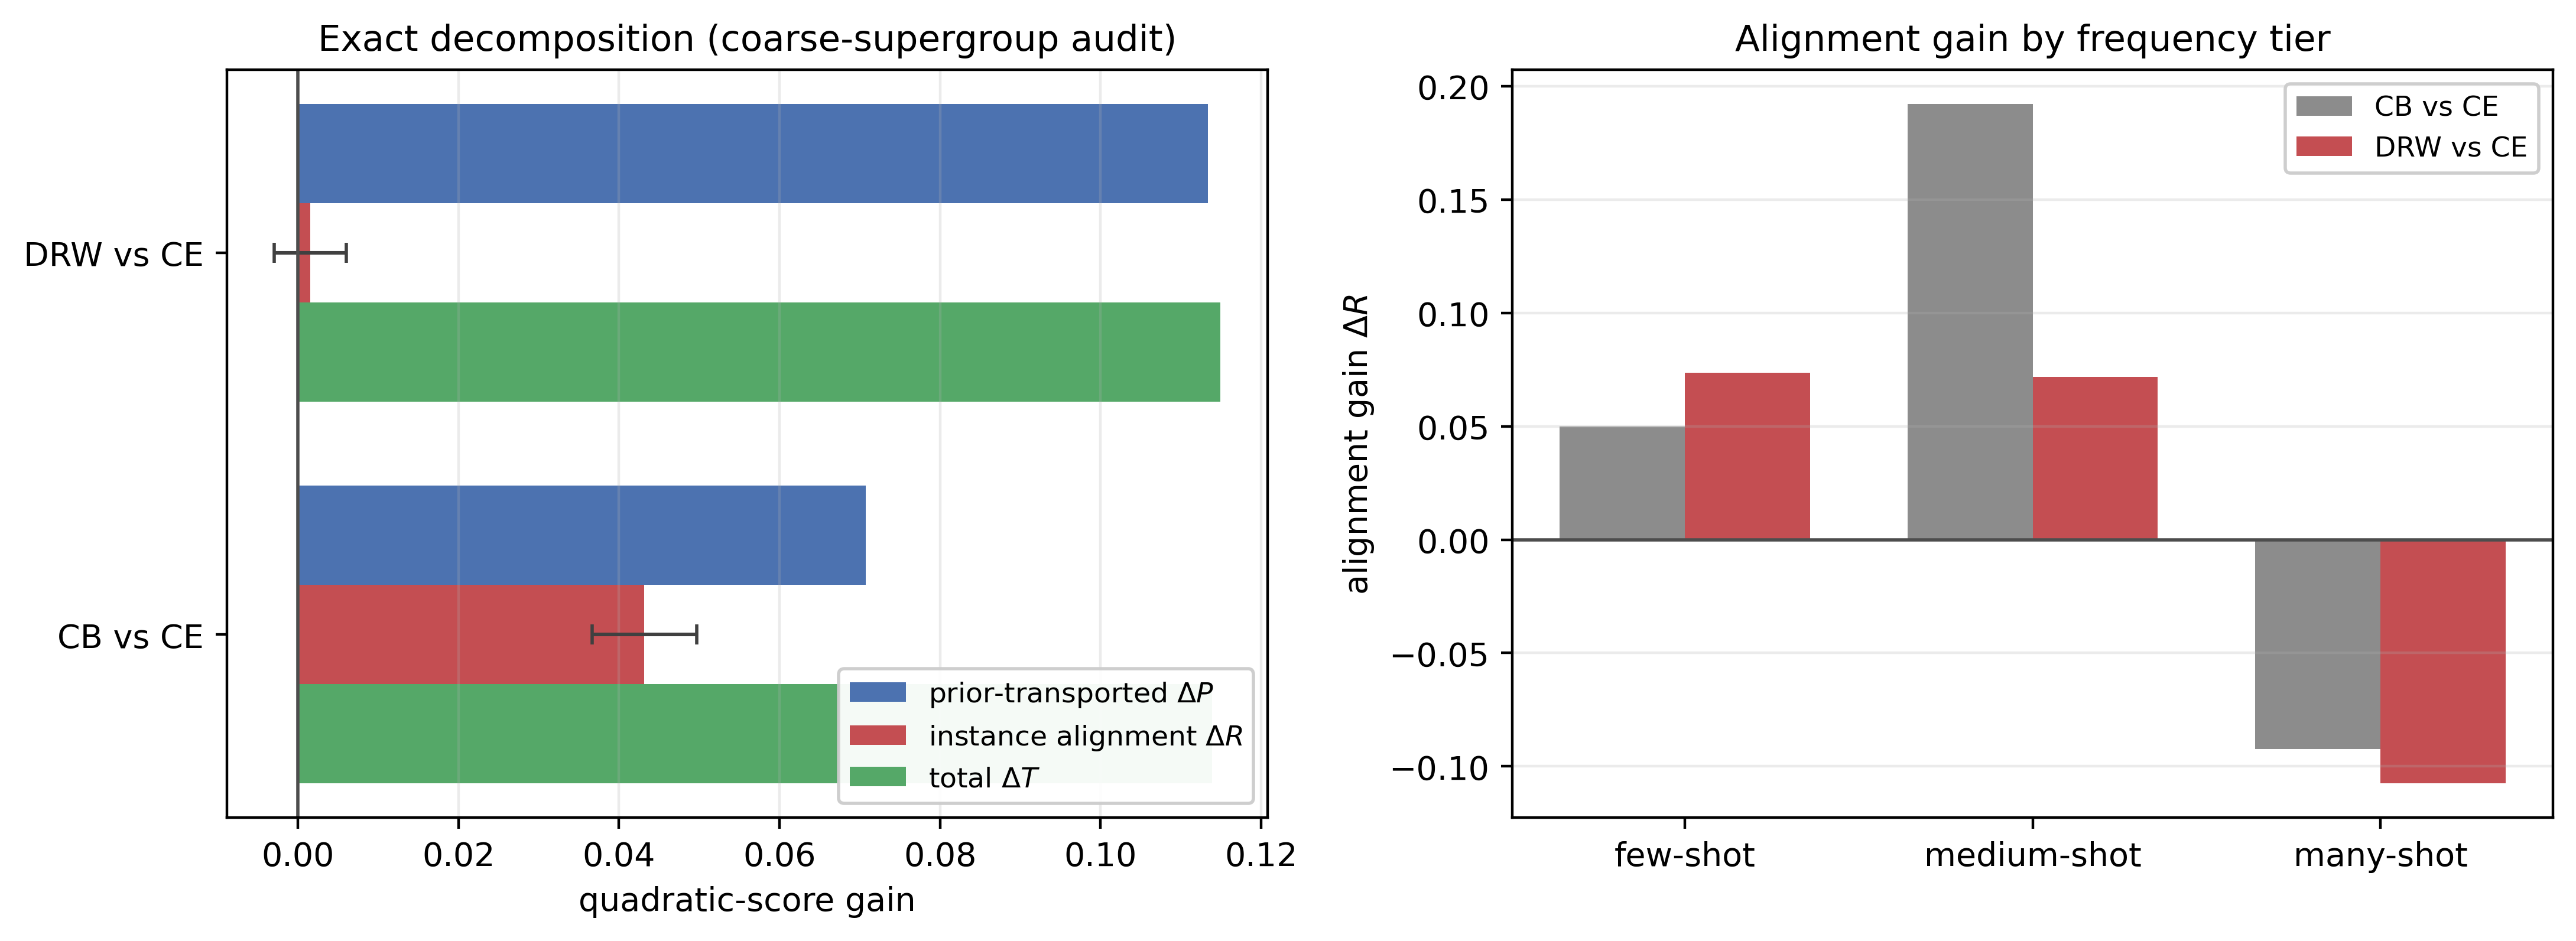
\includegraphics[width=\textwidth]{figures/fig8_text_lt.png}
\caption{\textbf{A third domain, with neither a spatial nor a class-frequency prior.}
Left: exact decomposition at the coarse-topic audit; CB's total gain is genuinely split
between both channels while DRW's is almost entirely transported. Error bars are
95\% H\'ajek intervals on $\widehat{\Delta R}$. Right: covariance gain by
training-frequency tier for both schedules, showing the same head-loses/tail-gains
signature as Figure~\ref{fig:cifar} despite the change of domain and grouping variable.}
\label{fig:textlt}
\end{figure*}

Table~\ref{tab:textlt-tier} breaks the superclass-audit covariance down by
training-frequency tier for both schedules; the two methods agree in shape even though
their superclass totals diverge sharply in composition, each gaining covariance on rare
and medium-frequency categories and losing it on frequent ones, the same qualitative
signature Section~\ref{app:lt} reports for image classification.

\begin{table}[t]
\centering
\caption{Covariance gain by training-frequency tier at the superclass audit,
20-Newsgroups-LT. Both schedules gain within-group covariance on rare and medium categories
and lose it on frequent ones.}
\label{tab:textlt-tier}
\begin{tabular}{@{}lrrr@{}}
\toprule
Tier & $n$ & $\widehat{\Delta R}$, CB vs CE & $\widehat{\Delta R}$, DRW vs CE \\
\midrule
Few-shot ($<20$)          & 1954 & $0.04991$  & $0.07352$  \\
Medium-shot ($20$--$100$) & 2610 & $0.19213$  & $0.07171$  \\
Many-shot ($>100$)        & 2968 & $-0.09227$ & $-0.10753$ \\
\bottomrule
\end{tabular}
\end{table}

This third domain uses a single trained pair per schedule rather than the multi-seed,
calibration-matched protocol Section~\ref{app:lt} applies to CIFAR-100-LT; extending
that fuller protocol to text is the natural next replication, not a step this section
claims to have taken.


\end{document}
